\documentclass[12pt,fleqn]{report}                  % Times New Roman, 12pt
%\usepackage{gscale_thesis_singlespace} % Single spaced thesis
\usepackage{style_files/gscale_thesis_doublespace} % Double spaced thesis
\usepackage{style_files/fancyheadings}                   % Header and footer styling
\usepackage[square]{natbib}                               % Bibliography formatting
\usepackage{setspace}                           % Allows double spacing but skips headers/footers
\title{Leveraging Information Contained in Theory Presentations}
\halftitle{Leveraging Information Contained in Theory Presentation} % 60 Characters Max. Including Spaces

\author{Yasmine Sharoda}
\shortauthor{Y. Sharoda} % Used for page header

\dept{Computing and Software} % The department you are part of; Must be all lower case
\field{Computer Science} % What field your thesis is in

\prevdegreeone{M.Sc.}
\prevdegreetwo{M.Sc.} % Just your degree's field

\submitdate{January, 2021}
\copyrightyear{2021}

\principaladviser{Jacques Carette and William M. Farmer} % Your Supervisor
                                % LaTeX variables for preface pages/headers
\setcounter{tocdepth}{1}                        % Limits the TOC to chapter and section names
\setcounter{secnumdepth}{3}
% Additional packages
\usepackage{minted}
\usepackage{listings}
\usepackage[T1]{fontenc}
\lstset{basicstyle={\ttfamily}}%\footnotesize
\usepackage[show]{ed}
\usepackage{graphicx}                                   % Allows the inclusion of figures
\usepackage{subcaption}                               % Allows captions to be added to subfigures
\usepackage[justification=centering]{caption} % Centres caption text
\usepackage[breaklinks=true, colorlinks=true, linkcolor  = black, citecolor=blue]{hyperref}                    % Linking to LaTeX labels and external URLs
\usepackage{array}                                        % Used for table formatting
\newcolumntype{P}[1]{>{\raggedright\let\newline\\\arraybackslash\hspace{0pt}}m{#1}}
\usepackage{booktabs}                                 % Fancy-style tables
\usepackage{longtable}                                 % Allows for tables that are more than one page long
\usepackage{float}                                         % Better figure placement control
\usepackage{enumerate}   
\usepackage[shortlabels]{enumitem}                            % Numbered lists 
\usepackage[shortcuts]{extdash}                  % Allows manual hyphenation of hypenated words
\usepackage{amsmath}                                % Non-standard math symbols
\usepackage{amsfonts}                                % Extended fonts for 
%mathematics
\usepackage{xcolor}
\numberwithin{equation}{section}                 % Numbers equations based on their section

\usepackage{stmaryrd}
\usepackage{comment}
\usepackage{tikz}
\usetikzlibrary{arrows.meta, % for arrows style
                positioning  % for positioning of boxes
               }
\usepackage{tikz-cd}
\usepackage{multicol}
\usepackage{upgreek}
\usepackage{adjustbox}

\numberwithin{equation}{section}                 % Numbers equations based on their section
\usepackage{xspace}
\usepackage{MnSymbol}
\usepackage{proof}
\usepackage{prooftree1}
\usepackage{style_files/macros}
\usepackage{style_files/tpcj_macros}
\usepackage{style_files/combinators}

\providecommand\myscale{4.5}

\usepackage{supertabular}
\usepackage{ott/dtt}

\usepackage{url}
\def\UrlBreaks{\do\/\do-}

%\setcitestyle{authoryear,open={[},close={]}}

%\definecolor{ourblue}{rgb}{0.90,0.98,1.0}
%\definecolor{ourpink}{rgb}{1.0,0.96,0.99}
%\newcommand{\tog}{tog}
%\newcommand{\etc}{etc.}

% ********************************
\begin{document}
\begin{comment}
\beforepreface                                         % Half title page, title page, declaration page   
  %\include{layabstr}                                  % Lay Abstract
  \prefacesection{Abstract}

Building a large library of mathematical knowledge is a complex and labour-intensive task.
By examining current libraries of mathematics, we see that the human effort put in building them is not entirely directed towards tasks that need human creativity. 
Instead, a non-trivial amount of work is spent on providing definitions that could have been mechanically derived.

%Instead, a non-trivial amount is directed towards redefining basic mathematical knowledge. 
%Instead of focusing all the human effort on formalizing more knowledge, we find that some basic mathematical concepts are being redefined again and again based on changing design decisions. 

In this work, we propose a generative approach to library building, so definitions that can be automatically derived are computed by a meta-program. We focus our attention on libraries of algebraic structures, like monoids, groups, and rings. 
These structures are highly inter-related and their commonalities have been well-studied in universal algebra. We use theory presentation combinators to build a library of algebraic structures. Definitions from universal algebra and programming languages meta-theory are used to derive library definitions of constructions, like homomorphisms and term languages, from algebraic theory presentations. The result is an interpreter that, given $227$ theory expressions, builds a library of over $5000$ definitions. This library is, then, exported to Agda and Lean. 

%We use meta-programs to generate  

%where definitions that are normally provided by library developers are automatically generated by a meta-program. We focus our attention to algebra libraries. Algebraic theories are highly structured and their commonalities has been well-studied in universal algebra. We use theory presentation combinators to capture the structure of algebraic theories. Universal algebra definitions are used to derive definitions of constructions, like homomorphism and term languages, from algebraic theory presentations. The result is an interpreter that, given $227$ theory expressions, builds a library of over $5000$ definitions.


                                      % Abstract
  \include{dedic}                                      % Dedication
  \prefacesection{Acknowledgements}
\vspace{-1cm}
\begin{center} 
\textit{Praise and gratitude be to Allah, the most gracious and the most beneficent.}
%with the blessings whom the good deeds are fulfilled.
\end{center}
\noindent I would like to express my sincere thanks to my supervisors Dr.~Jacques Carette and Dr.~William Farmer for their continuous support to my learning journey.  Your expertise and feedback were invaluable in shaping this research direction and throughout my studies. 
I learned from you a lot about how to do research and communicate it. 
I am very thankful to Dr.~Wolfram Kahl and Dr.~Ridha Khedri for being on my supervisory committee. Your feedback, over the years, on this work is very appreciated. Many thanks to my external examiner, Dr. Makarius Wenzel, for the useful feedback and the interesting discussions. 

I am grateful to Dr.~Michael Kohlhase, Dr.~Florian Rabe, and members of the KWARC team for inviting me to their research group at FAU Erlangen. The collaboration between our teams has been a great source of inspiration for this work. 

I would like to express of my heartfelt appreciation to Dr. Andrea Kohlhase for her support and for being a great role model. 

Without the support of my family and friends, I wouldn't have been able to pursue this degree. Thanks for all the love and support. Thank you for always believing in me and encouraging me to explore different areas. 
I am most grateful to Ahmad, my husband, best friend and mentor. Thank you for always being there for me. I am so proud of the team we make. 
                 % Acknowledgements
 % \referencepageswithnotations{notation} % Table of Contents, List of Figures, List of Tables, Notations
  %\referencepages                                 % No notations version (choose one)
\afterpreface                
\end{comment}

\tableofcontents

\chapter{Introduction}
\label{ch:intro}

%Mathematical theorem provers comes equipped with libraries of formalized mathematics. 
A large library of formalized, ready-to-use mathematics has long been the pursuit of mathematicians and computer scientists.  
The influential QED manifesto~\citep{boyer1994qed}, released in 1994, envisioned a library in which all mathematics is formalized and rigorously checked. The QED manifesto believed in one-formalization-fits-all approach to building this library.
Diversity in mathematical formalizations was a big obstacle towards realizing the library described by QED. There was not an agreement even on which foundation to use for formalizing all of mathematics~\cite{qedrealoaded2016}.  Since then, mathematical knowledge management (MKM) became an active area of research framing a new vision for the large math library. The universal digital math library (UDML), described in~\cite{farmer2004mkm}, is a collection of heterogeneous, intercommunicating systems and building this library is described as a grand challenge facing MKM. 

Despite the many efforts dedicated to building math libraries\ednote{some references}, a universal large library has not become a reality. One reason is that developing and maintaining libraries of mathematics requires a lot of manpower. One would want to believe that this human effort is put into the creative work of formalizing new pieces of knowledge. By examining current libraries of theorem provers, we know this is not always the case. The process of creating libraries for theorem provers involve a lot of redundancy. We give examples from libraries of formal systems in Chapter~\ref{ch:redundancy}. To understand why this redundancy exists, we examine the formalization of \lstmath{Monoid} in algebra textbooks versus in interactive theorem provers. 

\lstmath{Monoid} is an algebraic structure that describes algebras with carrier set and associative binary operation over that set that has a unit. The definition given in~\cite{jacobson1985basic}  is 
\begin{quote}
    A monoid is a triple $(M,p,1)$ in which $M$ is a non-vacuous set, $p$ is an associative binary composition (or product) in $M$, and $1$ is an element of $M$ such that $p(1,a)= a = p(a,1)$ for all $a \in M$ 
\end{quote}
The definition of \lstmath{Monoid} is followed by the definition of its homomorphism as
\begin{quote}
If $M$ and $M^\prime$ are monoids, then a map $\eta$ of $M$ into $M^\prime$ is called a homomorphism if 
\begin{multicols}{3}
    $\eta(ab)=\eta(a)\eta(b)$, \vfill   
    \columnbreak
    $\eta(1) = 1$, \vfill   
    \columnbreak 
    $a,b \in M$  \vfill    
\end{multicols}
\end{quote}
More monoid-related constructions are defined, like submonoid, and quotient monoids. The same constructions are defined for \lstmath{Group} and \lstmath{Ring}. 
%Mathematics presented in textbooks rely on the human understanding to be able to generalize these concepts. For example, \cite{jacobson1985basic} does not provide an explicit definition for group homomorphism, but proceeds to use it. 

Formal systems\footnote{We use the term \emph{formal systems} to refer to all computer systems with logical foundations, be it automatic theorem prover (ATP), interactive theorem prover (ITP), specification system, or others.} present algebraic structures using axiomatic theories\ednote{should I define axiomatic theories?}. \lstmath{Monoid} and its homomorphism are presented axiomatically in a minimal (imaginary) computer language as follows 
\begin{lstlisting}[mathescape]
theory Monoid { 
  A : type 
  e : A
  op : A $\to$ A $\to$ A
  lunit : (x : A) $\to$ op e x = x 
  runit : (x : A) $\to$ op x e = x 
  assoc : (x y z : A) $\to$ op x (op y z) = op (op x y) z
}

theory MonoidHom { 
  M1, M2 : Monoid  
  hom : M1.A $\to$ M2.A 
  pres-e : hom (M1.e) = M2.e
  pres-op : (x y : M1.A) $\to$ hom (M1.op x y) = M2.op (hom x) (hom y) 
}
\end{lstlisting}
Let's now define \lstmath{Group} and \lstmath{Group} homomorphism within the same language
\begin{lstlisting}[mathescape]
theory Group {
  A : type 
  e : A
  op : A $\to$ A $\to$ A
  inv : A $\to$ A
  lunit_e : (x : A) $\to$ op e x = x
  runit_e : (x : A) $\to$ op x e = x
  linverse : (x : A) $\to$ op x (inv x) == e
  rinverse : (x : A) $\to$ op (inv x) x == e
  associative : (x y z : A) $\to$ op x (op y z) = op (op x y) z
}

theory GroupHom { 
  G1, G2 : Group 
  hom : G1.A $\to$ G2.A
  pres-e : hom (G1.e) = G2.e
  pres-op : (x y : G1.A) $\to$ hom (G1.op x y) = G2.op (hom x) (hom y)
  pres-inv : (x : G1.A) $\to$ hom (G1.inv x) = G2.inv (hom x)
}
\end{lstlisting}
Notice how the two definitions of homomorphisms are similar and do not depend so much on the details of the theory. Generally, the homomorphism of a theory \lstmath{X} is a mapping between two instances of \lstmath{X} and has $3$ components 1) the $2$ instances of the theory, 2) the function \lstmath{hom} that maps the carriers of the $2$ instances, and 3) preservation axioms \lstmath{pres-x} for every operation symbol \lstmath{x}. The preservation axioms follow the pattern
\begin{lstlisting}[mathescape]
hom (op$_1$ x$_1$ .. x$_n$) = op$_2$ (hom x$_1$) .. (hom x$_n$)
\end{lstlisting}
Observing this pattern gives rise to some questions
 
\begin{itemize}
\item[Q1] Is this pattern specific to \lstmath{Monoid}, \lstmath{Group}, and their homomorphisms? 
\end{itemize}    
\lstmath{Monoid} and \lstmath{Group} are two of many algebraic structures used in abstract algebra. The commonalities between these structures is the subject of study of universal algebra, and is captured by the following definition~\cite{mckenzie1987algebras}
\begin{quote}
    An algebra is an ordered pair $\langle A, F \rangle$ such that $A$ is a nonempty set and $F = \langle F_i : i \in I \rangle$ where $F_i$ is a finitary operation on $A$ for each $i \in I$. $A$ is called the universe of $\langle A, F \rangle$, $F_i$ is referred to as a fundamental or basic operation of $\langle A, F \rangle$ for each $i \in I$, and $I$ is called the index set of the set of operation symbols for $\langle A, F \rangle$. 
\end{quote}
\ednote{look for a text book that explicitly state axioms. The properties of the function symbols, which are mentioned in mathematics textbooks but not always stated, are stated as axioms in formal systems, and so we defined an algebraic theory to be a type ($\langle A, F \rangle$,$E$), where $E$ is the set of axioms.}
\todo{check the sanella software specification book for this definition. }

For every theory that fit in this definition, we have a uniform definition of homomorphism, subalgebra, quotient algebra, term language and others. 

\begin{itemize}
    \item[Q2] What meta theory is used? 
\end{itemize}
While libraries of mathematics contain many different pieces of mathematical knowledge, we choose to focus on abstract algebra. Mathematicians have already studied the commonalities in this field and created universal algebra to describe it. Hence, we have a strong meta theory to understand how the definitions relate to each other. On the other hand, the MKM community have not utilized these abstraction in library building. This is the gap we are trying to fill in this work.  

\begin{itemize}
    \item[Q3] Is there enough information that can be generated? 
\end{itemize}
There is a lot of information that can be generated for one algebraic structure.  We list X\ednote{find the number} of them in Section~\ref{sec:toBeGenerated}. There are also many algebraic structures used in mathematics and computer science. While the hierarchy the comes in mind usually is \\
\lstmath{Semigroup $\to$ Monoid $\to$ Group $\to$ Semiring $\to$ Ring}, there are many more and are structured in a more complex way, as we discuss in Chapter~\ref{ch:library}. 
The list in~\cite{jipsen} defines over $300$ structure. There are also many being used in the meta theory of programming languages, like \lstmath{Applicative} and \lstmath{Monad}. 
Algebraic software specification is another area that uses algebraic theories to describe software. The broad scope of software systems make us believe there is a lot of algebraic structures being produced by this community.  

\begin{itemize}
    \item[Q4] What abstractions are needed (barriers exists) to generate this knowledge?
\end{itemize}\todo{This question can be written in a better way}.  
\lstmath{Monoid} theory is one of those captured by this abstraction. We have given a definition of \lstmath{Monoid} in an imaginary language that fits in this abstraction. In Figure~\ref{fig:mon-diff-lang}, we show the definitions of \lstmath{Monoid} in $5$ different language. 
\begin{figure}
    \footnotesize
\begin{tabular}{p{6.3cm} p{7cm}}
\underline{Haskell}
\begin{minted}[mathescape]{haskell}
class Semigroup a => 
      Monoid a 
 where 
  mempty :: a 
  mappend :: a -> a -> a 
  mappend = (<>) 
  mconcat :: [a] -> a 
  mconcat = 
   foldr mappend mempty 
\end{minted} 
\underline{Lean}
\begin{leancode}
class monoid (M : Type u)
 extends semigroup M, 
         has_one M :=
  (one_mul : ~$\forall$~ a : M, 
           1 * a = a) 
  (mul_one : ~$\forall$~ a : M, 
           a * 1 = a)   
\end{leancode} 
% [mathescape=true, escape_inside=~~]
\underline{Coq}
\begin{minted}[mathescape=true, escapeinside=~~]{coq}
class Monoid {A : type}
 (dot : A ~$\to$~ A ~$\to$~ A)
 (one : A) : Prop := {
  dot_assoc : 
   forall x y z : A, 
   (dot x (dot y z)) = 
   dot (dot x y) z
  unit_left : forall x, 
   dot one x = x 
  unit_right : forall x, 
   dot x one = x              
}
~$\text{\textit{Alternative Definition:}}$~
Record monoid := {
 dom : Type; 
 op : dom -> dom -> dom 
  where "x * y" := op x y; 
 id : dom where "1" := id; 
 assoc : forall x y z, 
  x * (y * z) = (x * y) * z; 
 left_neutral : forall x,   
  1 * x = x; 
 right_neutal : forall x,
  x * 1 = x; 
}
\end{minted} 
&
\underline{Agda}
\begin{agdacode}
record Monoid c ~$\ell$~ : 
   Set (suc (c ~$\sqcup$~ ~$\ell$~)) where 
 infixl 7 _~$\bullet$~_
 infix 4 _~$\approx$~_
 field 
  Carrier : Set c 
  _~$\approx$~_ : Rel Carrier ~$\ell$~ 
  _~$\bullet$~_ : Op~$_2$~ Carrier 
  isMonoid : IsMonoid _~$\approx$~_ _~$\bullet$~_ ~$\varepsilon$~ 
  
record IsMonid (~$\bullet$~ : Op~$_2$~) (~$\varepsilon$~ : A) 
 : Set (a ~$\sqcup$~ ~$\ell$~) where 
  field 
   isSemiring : IsSemiring ~$\bullet$~ 
   identity : Identity ~$\varepsilon$~ 
       
   open IsSemigroup isSemigroup public 
   
   identity~$^l$~ : LeftIdentity ~$\varepsilon$~ ~$\bullet$~ 
   identity~$^l$~ = proj~$_1$~ identity 
   identity~$^r$~ : Rightdentity ~$\varepsilon$~ ~$\bullet$~ 
   identity~$^r$~ = proj~$_2$~ identity        
\end{agdacode}       
\underline{MMT}
\begin{minted}[mathescape=true, escapeinside=~~]{mmt} 
theory Semigroup : ?NatDed = 
 u : sort 
 comp : tm u ~$\to$~ tm u ~$\to$~ tm u 
  # 1 * 2 prec 40
 assoc : ~$\vdash$~ ~$\forall$~ [x, y, z]
  (x * y) * z = x * (y * z)    
 assocLeftToRight : 
  {x,y,z} ~$\vdash$~ (x * y) * z 
          = x * (y * z) 
  = [x,y,z] 
   allE (allE (allE assoc x) y) z
 assocRightToLeft : 
  {x,y,z} ~$\vdash$~  x * (y * z) 
           = (x * y) * z 
  = [x,y,z] sym assocLR 
theory Monoid : ?NatDed 
 includes ?Semigroup 
 unit : tm u # e 
 unit_axiom : ~$\vdash$~ ~$\forall$~ [x] = x * e = x       
\end{minted}      
\end{tabular}  

    \caption{Representation of \lstinline|Monoid| theory in different languages.}
    \label{fig:mon-diff-lang}
\end{figure}
Although the $5$ definitions refer to the same mathematical concept, they look very different. The reason is that every system employ different design decisions. In some cases, as in Haskell and MMT, the theory \monoid is defined as an extension of \semigroup. Despite this being useful, there is no reason why a developer might not want to add a theory \unital (a non-associative \monoid), to the hierarchy. Exposing this hierarchy to the user makes their code vulnerable in case the hierarchy changes. This problem occurred when Haskell changed the hierarchy of type classes when \lstmath{Applicative} became a superclass for \lstmath{Monad} ~\cite{wiki:haskell_hierarch}. The work in \cite{cohen2020hierarchy} discusses this problem. The two Coq definitions takes two extreme views to the bundling problem~\cite{lean2019,alhassy2019,spitters2011type} by either having the carrier and all the function symbols as arguments (the first definition) or having all elements of the theory as declarations of a record type (the second definition). 
The formalization of the Algebraic hierarchy in the Agda standard library is based on setoids (sets equipped with the equivalence relation). Therefore, we find an extra field of the definition of \monoid corresponding to the equivalence relation $\_\approx\_$. 

Not only are library definitions diverse, but so are user projects. When design decisions are embedded that much into the definitions of the library, users find it difficult to reuse it in their projects and are forced to redefine many pieces. That leads to many libraries formalizing the same knowledge, even in the same language. Coq has at least $4$ different algebra libraries~\cite{Gonthier2009,Geuvers2002,coq-contribs-algebra,Spitters2010}. In~\cite{Gonthier2009}, the authors mention, referring to other libraries:  
\begin{quote}
    ``In spite of this body of prior work, however, we have found it
    difficult to make practical use of the algebraic hierarchy in our project to
    formalize the Feit-Thompson Theorem in the Coq system."
\end{quote}

This kind of redundancy is addressed in this thesis using generative programming. We define an abstraction over design decisions, from which different constructions defined by universal algebra can be automatically generated. By minimizing the design decisions that are embedded into the definition we aim to reduce redundancy and increase usability. 



\begin{comment}
\begin{itemize}
\item[Q3] What tools are needed to generate this information?  
\end{itemize}
We need a language to capture the abstractions of universal algebra, and meta programming capabilities to enable manipulating them to automatically generate new ones. 

When choosing the language, we don't want to be burdened with system-specifc details. We want to be as system independent as possible, as our ideas should apply to all systems that are able to represent first order theories. We see in Figure XX that normal practice of theory definition in many systems have design decisions embedded in the definition of the theory. We choose Tog~\cite{tog}, a minimal dependently types system to implement our ideas. We introduce it in Chapter~\ref{ch:tog}.  
\end{comment}

\section{Research Problem}
Our work contributes to the efforts of building large library of mathematics. The problem we are solving is that human developers manually provide definitions of constructions related to algebraic structures that are mathematically known to have definitions in terms of the structure. This suggest that we can have an algorithm that manipulates definitions of structures to produce definitions of their related constructions. 

We define two sources of redundancy in algebra libraries 
\begin{itemize}
    \item Handwritten library definitions that can be automatically generated by manipulating the definitions of the algebraic structures. 
    \item Redundancy in defining algebraic structures in libraries of formal systems. 
\end{itemize}

Elevating this human effort is possible because of two main reasons 
\begin{itemize}
    \item Definitions are written in a formal language which provide uniform syntax for expressing information. 
    %By having a suitable way to manipulate theories, we can generate information from them. This can happen if theories are first class citizens, if the needed reflection mechanisms are in place, or using a meta program in the hosting language. We use Tog~\cite{tog} as our language and type checker. We discuss Tog in Chapter~\ref{ch:tog}.  
    \item Universal algebra provides the definitions of many constructions in terms of the components of the algebraic structure. 
\end{itemize}
%This human work can be saved if universal algebra can be used to \emph{generate} some definitions. Many problems face this generative approach, some are 1) having design decisions baked into library definitions makes universal algebra abstractions not directly applicable, 2) Manipulating definitions require going to the meta-level using either strong reflection mechanisms or meta programs in the host language 

We suggest a generative approach in which a developer can \emph{describe} the information they need in the library and the design decisions they are employing, then library definitions get generated based on this description. This way we provide a domain specific langage (DSL) for theory development\ednote{introduce theory development}. 
\ednote{talk more about DSLs and why they are used}. 
%It would lift the burden of having to define utilities that are needed to perform the task in hand, but are standard information to the point that writing them is boring and distracting from the original task. 
%The DSL approach is useful in various ways. First, providing well-studied combinators to build algebraic theories can elevate their structure and connect them the right way, as we discuss in chapter~\cite{ch:library}. Also, library developers can use this DSL to generate parts of their library. Last, users of formal systems can use this DSL to automatically create utilities they need to get the systematic stuff done and focus on the novelty of their task. 

We are inspired by the \emph{deriving} mechanism in Haskell. When defining a new datatype, a Haskell user can ask for some utilities to be readily available for them to use on that type. The Haskell compiler would then generate these functions for the user. Some of these are basic, like equality and printer, but the community has gone as far as giving users the chance to define their own templates for deriving instances, knows as the \emph{deriving-via} technique. A pretty impressive example of deriving information is shown in Figure~\ref{fig:deriving-via-example}\ednote{find a better way to put the link to the source}. 
Also, the Lens library~\cite{lensesLib} in Haskell, use template Haskell~\cite{sheard2002TH} for the same purpose. 
\begin{figure}
    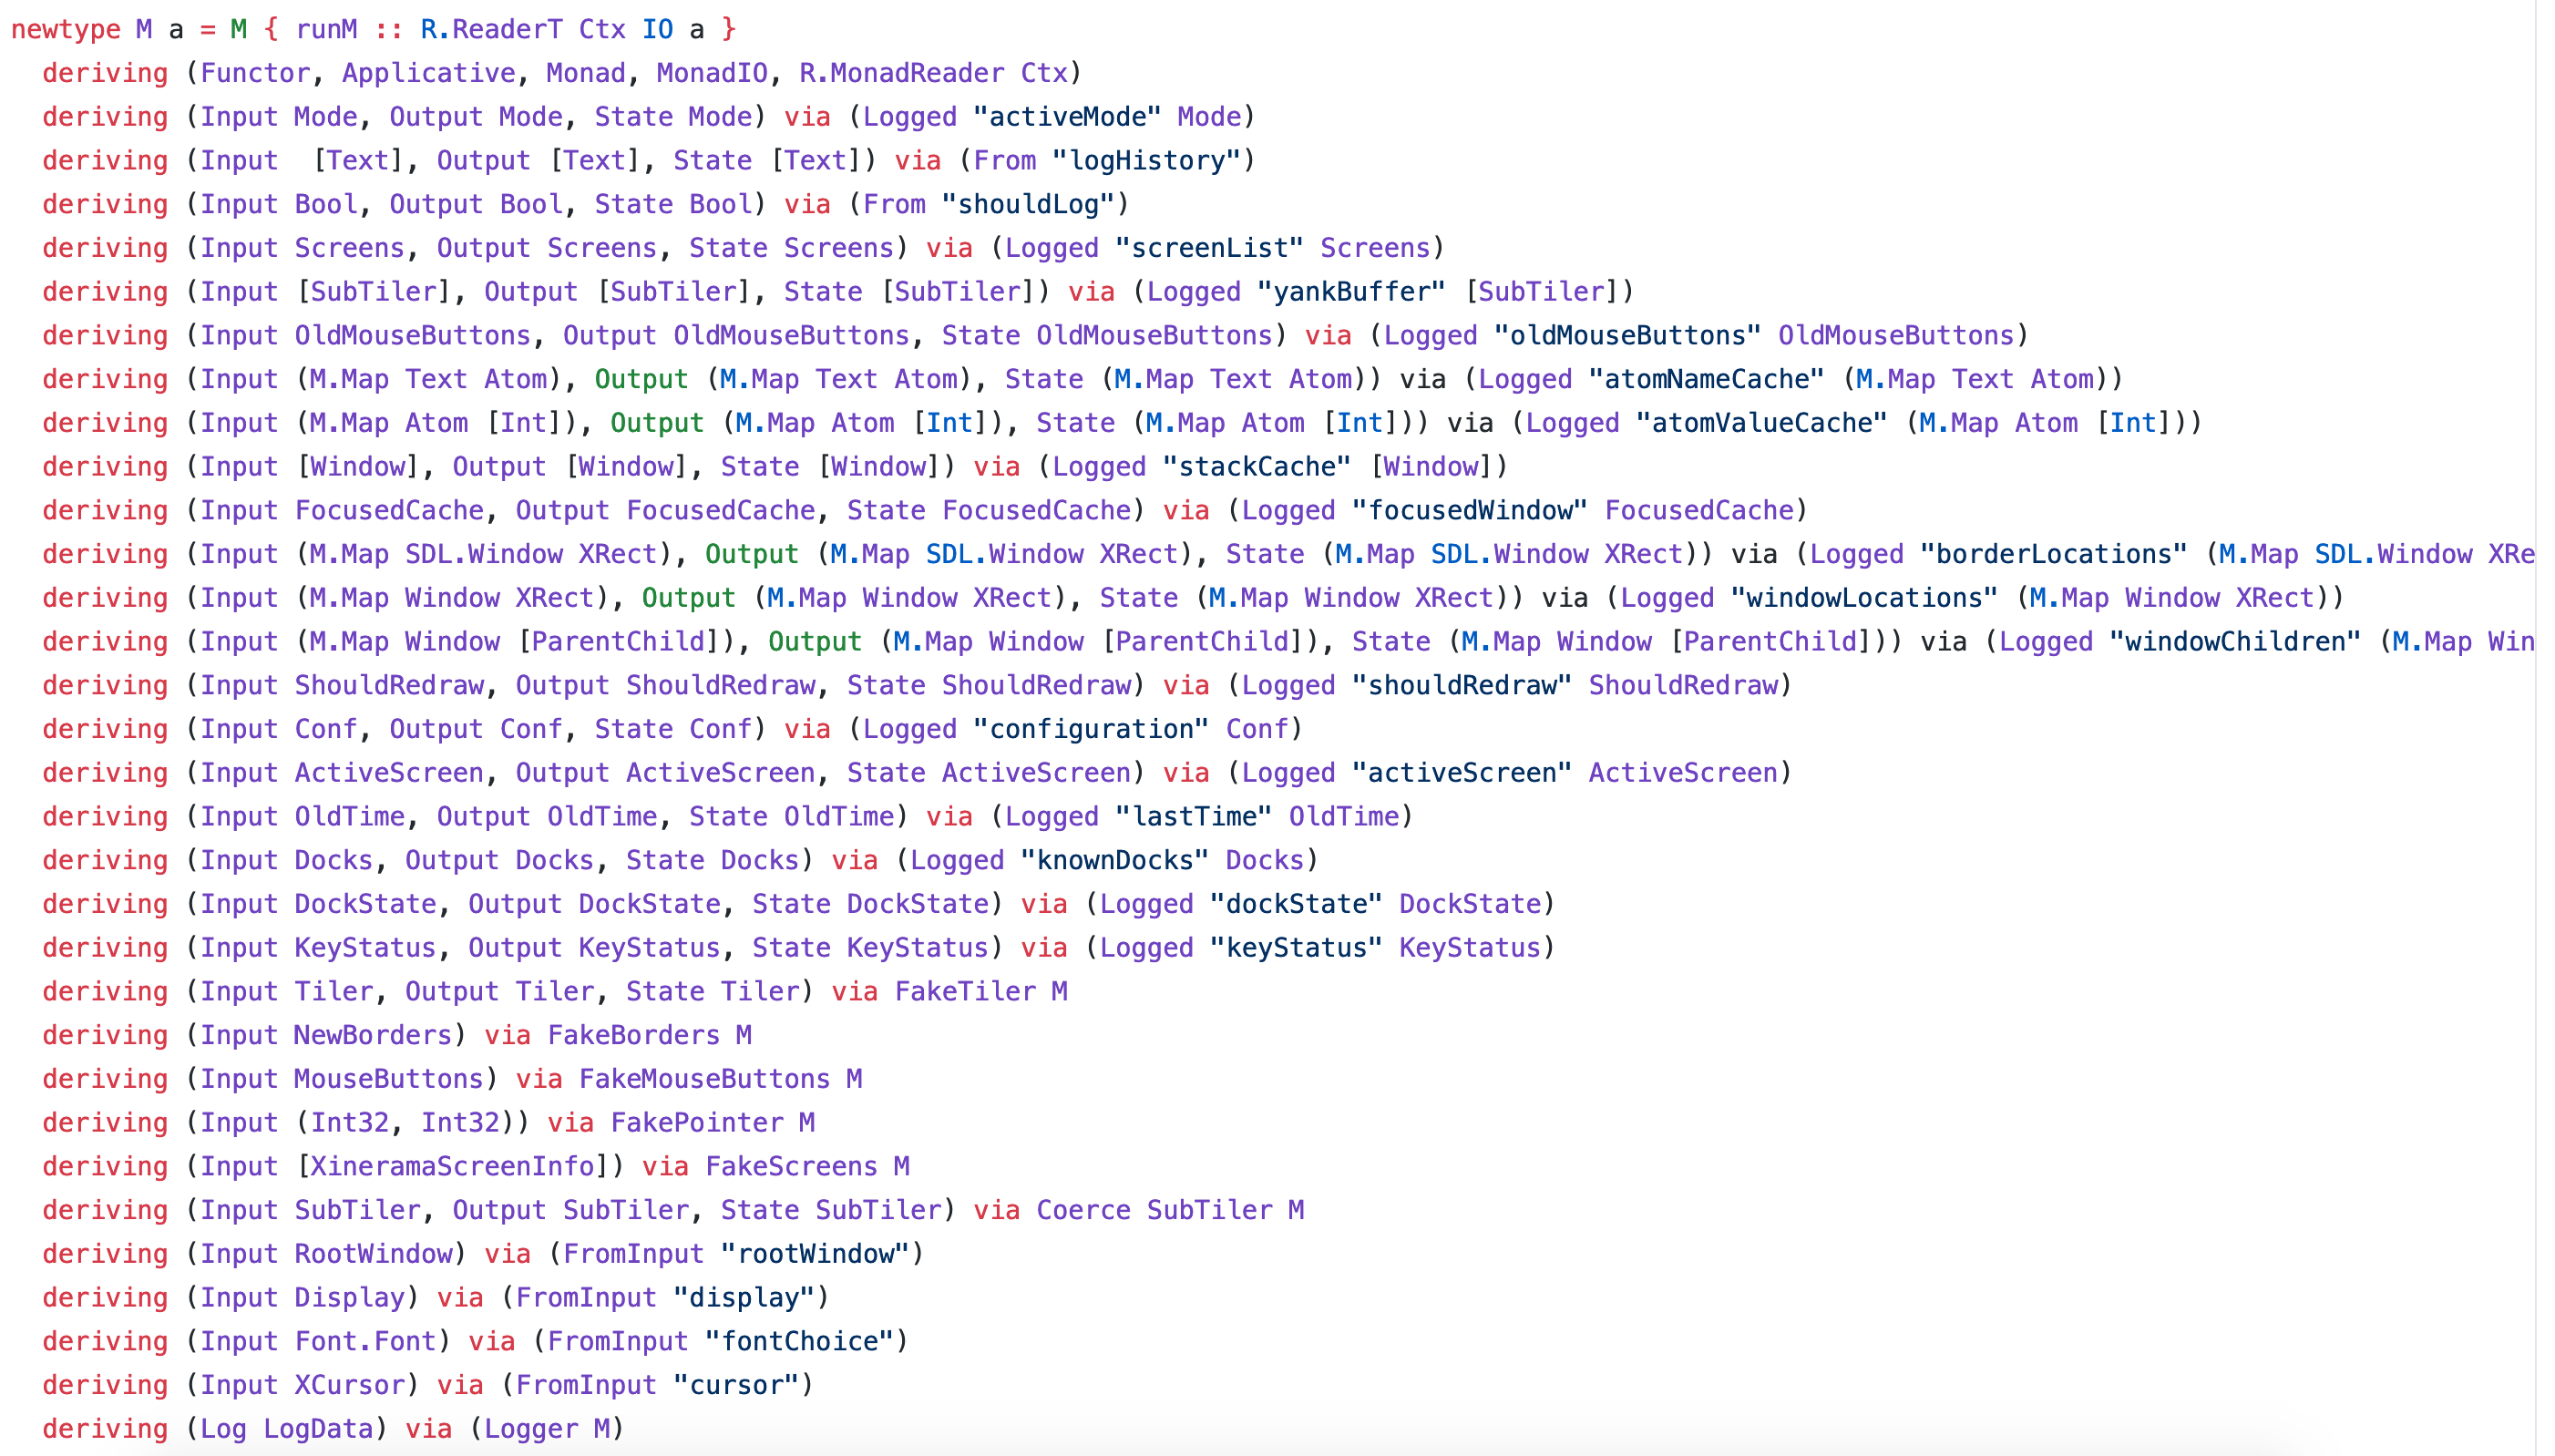
\includegraphics[scale=0.5,width=\linewidth]{figures/deriving-via-example.png}
    \caption{Example of deriving information in Haskell. source:\url{https://github.com/jhgarner/Xest-Window-Manager/blob/3741b35a69eb2cf8cd7320e186fd40134d1c1a56/src/Base/DoAll.hs}}
    \label{fig:deriving-via-example}
\end{figure}

This DSL would change the activity of theory development in the following way 
\begin{itemize}
    \item Save the human effort put in reproducing standard knowledge by internalizing this knowledge in the generation algorithm.
    \item Maintain a level of flexibility towards changing design decisions by understanding how they affect the generated definitions.
    \item Increase the usability of library definitions by reducing the amount of design decisions baked into them. 
\end{itemize}  

%The definitions we use in our development are based on universal algebra abstractions. Universal algebra abstracts over algebraic structures and their related constructions and provides the meta theory that explains how the generation algorithms should work. A theory presentation in universal algebra has three components \verb|(S,F,E)|; a sort \verb|S|, a list of function symbols along with their types \verb|F|, and a list of axioms (equations) that describe properties of the function symbols \verb|E|. If we can abstract over the details of theory presentations to extract this information, we are able to generate the constructions defined by universal algebra, like morphisms, product algebras, term languages, and others. 

In this work, we attempt to answer the following research questions\todo{refer to the questions later, make sure they are all addressed in the thesis and the conclusion} 
\begin{enumerate}
    \item[RQ1] Can the uniformity provided by universal algebra be captured by a meta program that generates parts of an algebra library?
    \item[RQ2] What design decisions need to be abstracted from and which ones can be reintroduced after the generation of new?
    \item[RQ3] Which information need to be provided by the developer and which ones can be generated? 
    \item[RQ4] What are the preconditions for generating this new information? 
    \item[RQ5] How would this affect the activity of library building?
    \item[RQ6] Can these generation algorithms be extended beyond uni-sorted first-order theories, the ones that universal algebra captures? 
\end{enumerate}

\section{Contributions}
\todo{forward reference to chapter+section where contribution is documented}
\begin{itemize}
    \item Highlight the redundancy in algebra libraries
    \item Compile a list of structures that can be generated from theory presentations
    \item Generate some of these constructions in Tog, a small implementation of a dependently typed language, in the style of Agda, Coq and Lean. 
    \item Export this implementation to Agda 
    \item Test our framework on a library of over $200$ theories implemented using the combinators defined in~\cite{carette2018building}. 
\end{itemize}  

\section{Broader Context}\todo{Make a bridge to it being broader context, readers say they don't see the context}. 
\label{sec:broader_context}
There are different ways of organizing knowledge within a formal system. Our work contributes to building a large math library organized as a theory graph in the heart of a tetrapodal structure. Theory graphs, explained in details in Section~\ref{sec:background:theorygraph}, capture the structure of mathematical knowledge by enabling the description of relationships between the different pieces using morphisms. Using them, we can express facts like `a group is a monoid` and that `monoid and additive monoid are isomorphic`. 

The nodes of a theory graph can be any kind of theories. Ideally, they would be biform theories~\cite{biformCICM2018}, as they connect axiomatic theories (used by theorem provers), and algorithmic theories (used by computer algebra systems) using meaning formulas. That way it facilitates communication between reasoning and computational systems; it becomes possible to reason about algorithmic theories, and to use results of computer algebra systems in theorem provers. In this work we only look at axiomatic theories. 

Morphisms are meaning preservation maps. The simplest form of a morphism is inclusion. Morphisms are used to transfer results from one theory to another. So, a morphism between \lstmath{Monoid} and \lstmath{AdditiveMonoid} that describes they are isomorphic, allows us to transfer results between them. 

In~\cite{carette2020bigMath}, the authors argue that modern mathematics is organized as a tetrapod with knowledge organization being at its center. We are working towards a library organized as a theory graph of biform theories that serves as this center. Different aspects of the tetrapod will be consumers and producers of knowledge in this library. This implies that the size of this library would be huge, and that using generative approach to support its building would be a great asset. 

We support the building of this library by providing combinators to define the library theories and algorithms to compute related constructions

\section{Publications}
This thesis lead to the following publications\ednote{how should I refer to myself here, I? the author?}\todo{write my contribution in~\cite{biformCICM2018}}\ednote{should I also include the abstract submitted to CICM2019 doctoral program?}: 
\begin{itemize}
    \item In \cite{biformCICM2018},
    \item The MathScheme library is built using combinators that has been first published in~\cite{CaretteOConnorTPC}. The author contributed to an extended version of the paper, submitted to iournal of automated reasoning\cite{carette2018building}. The author's contribution to this work can be summarized as follows: 
    \begin{itemize}
        \item Taking part in developing the type system for the combinators 
        \item Surveying theory expressions in different formal systems to frame the novelty of the paper. 
        \item Providing the first arrow-based implementation of the paper, as we discuss in Section~\ref{sec:lib_implementation}. 
        \item Using the combinators to build a library of over $200$ theories. Although the library definitions pre-existed, many of them were not correct because they were based on theories. Shifting the implementation to arrows mandated figuring out the right arrows to build the theories, which was never done before this work.
    \end{itemize}
    \item ~\cite{diagrams_mmt} discusses diagram combinators in MMT~\cite{MMT}. We used the diagram combinators to implement the MathScheme library~\cite{mathscheme2011experiments}. This was our first attempt to implement the combinators and also the first time diagrams combinators is tested. As the combinators computes a theory and some arrows, we considered treating them as diagrams. There were promising results, but did not scale up as - by that time - there were problems with how MMT supports the diagram combinators. 
    \item In \cite{leverageCICM2020}, we present redundancy in libraries of formal systems, as well as our approach to generate many of those redundant definitions. The author collected the examples of redundancy, implemented the framework, and made most of the paper writing.
    \item The paper~\cite{bercic2020space} surveys the software used by producers and consumers of mathematical knowledge, categorizing them in $5$ different aspects; inference, computation, concretization, narration, and organization. The author contributed mainly to the organization aspect, finding how to best categorize how different system organize knowledge within them. 
\end{itemize}

\section{Outline}
\todo{This section}

\begin{comment}  
These algebraic concepts are very important in mathematics and computer science that they are a main component in libraries of almost every mechanized system\ednote{add citations on research of algebra library development}. We consider the \lstmath{Monoid} structure for our running example. a \lstmath{Monoid} consists of a carrier over which there is an associative binary operation that has a unit. If we look at algebra textbooks, we find that~\cite{mckenzie1987algebras} defines it as 
\begin{quote}%[mathescape]
A monoid is an algebra $A = \langle \cdot^A, e^A \rangle$ such that 
$\langle A, \cdot^A \rangle$ is a semigroup and \\
$a \cdot^A e^A = e^A \cdot^A a = a$ for all $a \in A$.
\end{quote}
In~\cite{jacobson1985basic}, it is defined as 


Algebra text books would follow the definition of an algebraic structure with the definitions of some of its related constructions, like subalgebras, homomorphisms, term languages, quotients, etc. The scope of the book might determine which ones are included. \cite{jacobson1985basic} provides the following definition of monoid homomorphism 

and proceeds to talk about \lstmath{Group} homomorphism depending on the human ability to infer it from its given definition of \lstmath{Monoid}. 

Moving to formal systems, We find that they also do not agree on one definition of the theory \lstmath{Monoid}. Figure~\ref{fig:mon-diff-lang} shows its definition in $5$ different languages. 
\begin{figure}
\footnotesize
\begin{tabular}{p{6.3cm} p{7cm}}
\underline{Haskell}
\begin{minted}[mathescape]{haskell}
class Semigroup a => 
      Monoid a 
 where 
  mempty :: a 
  mappend :: a -> a -> a 
  mappend = (<>) 
  mconcat :: [a] -> a 
  mconcat = 
   foldr mappend mempty 
\end{minted} 
\underline{Lean}
\begin{leancode}
class monoid (M : Type u)
 extends semigroup M, 
         has_one M :=
  (one_mul : ~$\forall$~ a : M, 
           1 * a = a) 
  (mul_one : ~$\forall$~ a : M, 
           a * 1 = a)   
\end{leancode} 
% [mathescape=true, escape_inside=~~]
\underline{Coq}
\begin{minted}[mathescape=true, escapeinside=~~]{coq}
class Monoid {A : type}
 (dot : A ~$\to$~ A ~$\to$~ A)
 (one : A) : Prop := {
  dot_assoc : 
   forall x y z : A, 
   (dot x (dot y z)) = 
   dot (dot x y) z
  unit_left : forall x, 
   dot one x = x 
  unit_right : forall x, 
   dot x one = x              
}
~$\text{\textit{Alternative Definition:}}$~
Record monoid := {
 dom : Type; 
 op : dom -> dom -> dom 
  where "x * y" := op x y; 
 id : dom where "1" := id; 
 assoc : forall x y z, 
  x * (y * z) = (x * y) * z; 
 left_neutral : forall x,   
  1 * x = x; 
 right_neutal : forall x,
  x * 1 = x; 
}
\end{minted} 
&
\underline{Agda}
\begin{agdacode}
record Monoid c ~$\ell$~ : 
   Set (suc (c ~$\sqcup$~ ~$\ell$~)) where 
 infixl 7 _~$\bullet$~_
 infix 4 _~$\approx$~_
 field 
  Carrier : Set c 
  _~$\approx$~_ : Rel Carrier ~$\ell$~ 
  _~$\bullet$~_ : Op~$_2$~ Carrier 
  isMonoid : IsMonoid _~$\approx$~_ _~$\bullet$~_ ~$\varepsilon$~ 
  
record IsMonid (~$\bullet$~ : Op~$_2$~) (~$\varepsilon$~ : A) 
 : Set (a ~$\sqcup$~ ~$\ell$~) where 
  field 
   isSemiring : IsSemiring ~$\bullet$~ 
   identity : Identity ~$\varepsilon$~ 
       
   open IsSemigroup isSemigroup public 
   
   identity~$^l$~ : LeftIdentity ~$\varepsilon$~ ~$\bullet$~ 
   identity~$^l$~ = proj~$_1$~ identity 
   identity~$^r$~ : Rightdentity ~$\varepsilon$~ ~$\bullet$~ 
   identity~$^r$~ = proj~$_2$~ identity        
\end{agdacode}       
\underline{MMT}
\begin{minted}[mathescape=true, escapeinside=~~]{mmt} 
theory Semigroup : ?NatDed = 
 u : sort 
 comp : tm u ~$\to$~ tm u ~$\to$~ tm u 
  # 1 * 2 prec 40
 assoc : ~$\vdash$~ ~$\forall$~ [x, y, z]
  (x * y) * z = x * (y * z)    
 assocLeftToRight : 
  {x,y,z} ~$\vdash$~ (x * y) * z 
          = x * (y * z) 
  = [x,y,z] 
   allE (allE (allE assoc x) y) z
 assocRightToLeft : 
  {x,y,z} ~$\vdash$~  x * (y * z) 
           = (x * y) * z 
  = [x,y,z] sym assocLR 
theory Monoid : ?NatDed 
 includes ?Semigroup 
 unit : tm u # e 
 unit_axiom : ~$\vdash$~ ~$\forall$~ [x] = x * e = x       
\end{minted}      
\end{tabular}  

\caption{Representation of \lstinline|Monoid| theory in different languages.}
\label{fig:mon-diff-lang}
\end{figure}
For now, we imagine a definition of \lstmath{Monoid} in a simple language as follows 
\begin{lstlisting}[mathescape]
theory Monoid { 
A : type 
e : A
op : A $\to$ A $\to$ A
lunit : $\cdots$
runit : $\cdots$
assoc : $\cdots$ 
}
\end{lstlisting}        
The homomorphism of \lstmath{Monoid} in the same language is 
\begin{lstlisting}[mathescape]
theory MonoidHom { 
M1, M2 : Monoid  
hom : M1.A $\to$ M2.A 
pres-e : $\cdots$
pres-op : $\cdots$
}
\end{lstlisting}
The components of the homomorphism are $2$ instances of \lstmath{Monoid} theory, a mapping from the carrier of one instance to the other, and preservation axiom for every function symbols that follow the pattern 
\begin{lstlisting}[mathescape]
hom (op$_1$ x$_1$ .. x$_n$) = op$_2$ (hom x$_1$) .. (hom x$_n$)
\end{lstlisting}
Notice how all these components can be derived from the definition of \lstmath{Monoid}. 

Another commonly used algebraic structure is \lstmath{Group}. In order to use it in a formal system, one needs to define it along with all its related definitions that they need, like \lstmath{Group} homomorphism which follows the same pattern described above. This observation lead us to the question 
\end{comment}



\begin{comment}
Notice how all the 
~\cite{mckenzie1987algebras} is 
\begin{quote}%[mathescape]
A monoid is an algebra $A = \langle \cdot^A, e^A \rangle$ such that 
$\langle A, \cdot^A \rangle$ is a semigroup and \\
$a \cdot^A e^A = e^A \cdot^A a = a$ for all $a \in A$.
\end{quote}
Note how \lstmath{Monoid} is defined in terms of a smaller theory \lstmath{Semigroup}. While inthe definition given is  

In this case, \lstmath{Monoid} is defined in terms of its components. Both ways of defining \lstmath{Monoid} are useful and humans can switch between these definition without overhead. Depending on the task intended by the user, they might have a preference of one over the other. 
\end{comment}


%We focus our attention to algebra libraries which formalizes core concepts in mathematics and computer science. Algebra libraries contain axiomatic formalization of algebraic structures. Those structures describe classes of algebras. For example the algebras $(\mathbb{N},+,0)$ and $(Strings,++,\varepsilon)$ have similar behavior that is captured with the algebraic structure \lstmath{Monoid}. Defining and proofing properties of a structure is enough to define/prove it to all its models (all the algebras it describes). In the process of working with algebraic structures, one need some constructions related to them, like homomorphism, subalgebras, term algebras, etc. 


\chapter{Background}

\section{Axiomatic Theory}

A theory is a specification of a class of algebras, that share some properties. 
An axiomatic theory is a pair \lstmath{(L,$\Sigma$)}, where \lstmath{L} describes the language of the theory. It consists of \lstmath{(S,F)}. \lstmath{S} is a set of sorts and \lstmath{F} is a set of function symbols. \lstmath{$\Sigma$} is a set of axioms describing properties of objects in the language. A theory is closed under logical consequences, therefore we speak of a \emph{theory presentation}, in which only necessary axioms are given. Theory presentations are defined in a logic that provides the inference rules used to derive useful theorems.  

In a dependently typed setup, the distinction between sorts, functions symbols, and axioms need not exist. Instead a theory is seen as a telescope~\cite{de1991telescopic}. Every declaration \lstmath{$c : t$} within the telescope is defined within a context \lstmath{$\Gamma$}. This is described as \lstmath{$\Gamma \vdash c : t$}.  

A theory presentation is well-typed if every declaration \lstmath{$c : t$} is well-typed given its context. The formation rules for theory presentations are given in Figure~\ref{fig:ctx}, where $\syms{\Gamma}$ refers to the list of symbols defined in the context $\Gamma$. 
$$ \syms{\context{\varnothing}} = \EmptyThy \qquad
\syms{\context{\Gamma}\ ;\ x : \sigma} = \syms{\context{\Gamma}} \cup \left\{ x \right\}
$$
\begin{figure}[ht]
    \begin{proofrules}
        \[ \ \justifies \varnothing \ \wfctx \]
        \[ \context{\Gamma}\ \wfctx \qquad \sigma \notin \syms{\context{\Gamma}}
        \qquad \context{\Gamma} \vdash \kappa : \Box \justifies
        (\context{\Gamma}\ ;\ \sigma : \kappa)\ \wfctx \]
        \[ \context{\Gamma}\ \wfctx \qquad x\notin \syms{\context{\Gamma}}
        \qquad \context{\Gamma} \vdash \sigma : \kappa : \Box \justifies
        (\context{\Gamma}\ ;\ x : \sigma)\ \wfctx \]
    \end{proofrules}
    \caption{Formation rules for contexts as introduced in~\cite{carette2018building}}
    \label{fig:ctx}
\end{figure}

\section{Theory Morphisms}
\label{sec:morphisms}
Morphisms are used to capture the structure of mathematics, by describing how theories are related to each other. In mathematical texts, a theorem proved for an arbitrary \lstmath{Monoid} would be used when considering an arbitrary \lstmath{Group} without extra work. In formal mathematics, this can only be done if a morphism between \lstmath{Monoid} and \lstmath{Group} exists. The morphism specifies how results in \lstmath{Monoid} can be interpreted in \lstmath{Group}. 

A morphism $\arrow{[v]}{\Gamma}{\Delta}$ consist of a list of assignments $[v]$, a source theory \lstmath{$\Gamma$}, and a target theory \lstmath{$\Delta$}. $[v]$ assigns to every symbol in $\Gamma$ an expression of $\Delta$. A term \lstmath{t} in the language of $\Gamma$ can be translated into a term \lstmath{t$^\prime$} in the language of $\Delta$ using substitution, such that  \lstmath{t$^\prime$ = t$[v]$}. 

The formation rules for views, as given in~\cite{carette2018building} is given in Figure~\ref{fig:views}. 
\begin{figure}[ht]
    \begin{proofrules}
        \[ \context{\Delta}\ \wfctx \justifies \view{}{\varnothing}{\Delta} \]
        \[ (\context{\Gamma}\ ;\ x : \sigma)\ \wfctx \qquad
        \view{v}{\Gamma}{\Delta} \qquad
        \context{\Delta} \vdash r : \substitution{\sigma}{v}{} \justifies
        \view{v,x \mapsto r}{(\context{\Gamma}\ ;\ x : \sigma)}{\context{\Delta}} \]
    \end{proofrules}
    \caption{Formation rules for morphisms.}
    \label{fig:views}
\end{figure}

It is worth mentioning that the mapping is only a part of the morphism. A morphism consists of the source and destination theories as well as the mapping. 

We distinguish between three type of morphisms 

\subsection{Identity Morphism}
\label{sec:idmorph}
If $\arrow{[v]}{\Gamma}{\Delta}$ is an identity morphism, then $[v]$ maps every symbol $x \in \syms{\Gamma}$ to itself. This implies that $[v]$ is a bijection and that $x[v] = x$. 

Identity morphisms between two theories if the source is included verbatim in the destination, like in the case when \lstmath{Group} is defined as an extension of \lstmath{Monoid}. It is the simplest form of morphisms and allow transport of results without the need to perform substitution 

\subsection{Embedding}
\label{sec:embedding}
If $\arrow{[v]}{\Gamma}{\Delta}$ is an embedding, then $[v]$ is a bijection that maps every symbol $x \in \syms{\Gamma}$ to a symbol $r \in \syms{\Delta}$, which is not necessarily itself. 

Consider for example, the morphism from \verb|Magma| to \verb|AdditiveMagma|
\begin{equation*}\label{eq:additiveview}
\begin{tikzpicture}[node distance=9.0cm, auto,baseline=(current bounding box.center)]
\node (P) {$
    \begin{thyex}
    \thyrow{A}{\tmop{Type}}
    \thyrow{op}{A \rightarrow A \rightarrow A}
%    \thyrow{assoc_op}{\cdots}
    \end{thyex} $};
\node (B) [right of=P] {$
    \begin{thyex}
    \thyrow{A}{\tmop{Type}}
    \thyrow{+}{A \rightarrow A \rightarrow A}
%    \thyrow{assoc_+}{\cdots}
    \end{thyex} $};
\draw[->] (P) to node {$[A \mapsto\ A, 
    op \mapsto\ + ]$} (B);
\end{tikzpicture}
\end{equation*}
A term $t \in \Gamma$ is transported to $\Delta$ as $t[v]$, i.e.: by applying the substitution $[v]$ to the term $t$. 

\subsection{General Morphism}
\label{sec:generalmorph}
A morphism $\arrow{[v]}{\Gamma}{\Delta}$ is a general morphism if it maps symbols $x \in \syms{\Gamma}$ to terms $r \in \Delta$. 

An example is a morphism that flips a binary operation, i.e.: maps \lstmath{op x y} to \lstmath{op y x}
\begin{equation}\label{eq:flipmagmaview}
\begin{tikzpicture}[node distance=9.0cm, auto,baseline=(current bounding box.center)]
\node (P) {$
    \begin{thyex}
    \thyrow{U}{\tmop{Type}}
    \thyrow{op}{U \rightarrow U \rightarrow U}
    \end{thyex} $};
\node (B) [right of=P] {$
    \begin{thyex}
    \thyrow{U}{\tmop{Type}}
    \thyrow{op}{U \rightarrow U \rightarrow U}
    \end{thyex} $};
\draw[->] (P) to node {$[U \mapsto\ U,
    op \mapsto\ \mathsf{flip}\ op]$} (B);
\end{tikzpicture}
\end{equation}

\begin{comment}
 maps each symbol of \lstmath{$\Gamma$} to an expression in \lstmath{$\Delta$}. 

Statement in \lstmath{$\Gamma$} can be translated to statements in \lstmath{$\Delta$} via substitution.  some theory (source) into expressions of a destination theory. is mapping between two theories. this mapp

It maps symbols from the source theory to expressions in the target one. 
\end{comment}



\chapter{Universal Algebra}
\label{ch:ualgebra}
Algebraic structures, like monoids, groups, and rings, are classes of algebras that have similar properties. Universal algbera studies those structures in a more generic way. It abstracts over the specific definitions and properties of classes of algebraic structures and deals with them as axiomatic theories in equational first-order logic. With this abstraction in place, universal algebra defines some constructions useful when dealing with algebras and prove some of their properties.

We use concepts of universal algebra to leverage the information in theory presentations. We internalize a representation of uni-sorted equational first order theories into DTT, our meta theory. This way we are able to manipulate them and generate the constructions as described by universal algebra. In this chapter we introduce core concepts that we use from universal algebra. In Chapter~\ref{ch:generation} we discuss how we use it in our work. In Section~\ref{sec:eqtheory} we present equational first order logic, the meta theory for universal algebra, and define the components of a theory in this logic. We then introduce some of the constructions of universal algebra that can be generated from an equational theory presentation in Section~\ref{sec:toBeGenerated}. It is worth mentioning that although our framework generate only some of these constructions, they all follow from the definition of a theory and the definitions we provide here will hopefully make this noticeable.   

\section{Equational Theory}
\label{sec:eqtheory}
Logics give us the machinery to describe properties of entities as formulas and reason about them.  
Equational logic restricts these formulas, whether axioms or theorems, to be universally quantified equations of the form \lstmath{t$_1$ = t$_2$}, where \lstmath{t$_1$} and  \lstmath{t$_2$} are terms expressible in the language of the theory. There are different notions of equality~\cite{oneThingSame2008, equalityInTPs2015}. In many cases the underlying logic offers its own equality. In some other cases, the equality is defined by the language of the theory, as is the case with setoids. 

Equational logic has $3$ inference rules described in~\cite{Gries1993EquationalLogic}  
\begin{proofrules}
        \[ t_1 = t_2 \ \justifies t[x \mapsto t_1] = t[x \mapsto t_2] \]
        \[ t_1 = t_2 \qquad t_2 = t_3 \ \justifies t_1 = t_3 \]
        \[t \ \justifies t [xs \mapsto ts] \] 
\end{proofrules}       
\noindent where $t$, $t_1$, $t_2$, and $t_3$ are expressions, $x$ is a symbol in the language, $ts$ is a list of expressions, and $xs$ is a list of symbols. 
The leftmost rule refers to leibniz equality that states that two expressions are equal if one can be substituted by the other without changing the truth of a statement. 
The rule in the middle reflects the transitivity of equality. 
The rightmost rule states that if $t$ is true, then it remains true under all substitutions.  

%\section{A Theory in Equational Logic} 
%\label{sec:eqtheory}
A theory in universal algebra is described in first order equational logic. It restricts the definition of a theory described in Section~\ref{sec:background:theory}. It is defined as a tuple \lstmath{($\sort$,$\fsyms$,$\equations$)}
such that 
\begin{itemize}
\item $\sort$ is a set of one sort \lstmath{s}. 
\item $\fsyms$ is a finite set of function symbols. A $0$-ary function symbol is a constant. 
\item $\equations$ is a finite set of generating equations. 
\end{itemize}
%containing one sort .\footnote{In case of multi-sorted logics, the set $\sort$ is an indexed set of sorts. We restrict ourselves to unisorted logics as it captures the algebraic structures we're interested in, like monoids, groups, and rings.}
%An equation has the form \lstmath{t$_1$ = t$_2$}. We refer to this set as $\equations$, and therefore refer to a theory in equational logic as \lstmath{($\sort$,$\fsyms$,$\equations$)}. 
%An algebra describes a model  of the theory. It assigns a carrier set to the sort \lstmath{s} and functions to every symbol in $\fsyms$ such that the equations is $\equations$ hold. 

An algebra is a mathematical structure consisting of a domain and a set of functions on the domain. It provides an interpretation for the carrier $\sort$ and the function symbols in $\fsyms$ of a theory such that the equations in $\equations$ hold.  
%The models of a first-order algebraic theory presentation define algebras (1) whose domain and distinguished elements and functions are the interpretations of the carrier and symbols of the theory and (2) that satisfy the axioms of theory.  A model isn’t exactly an algebra.  It is a mapping to an algebra.

\section{Constructions}
\label{sec:toBeGenerated}
%Algebra makes the basis of many areas of computer science. We are interested in theorem proving and specification systems. \ednote{relate this to the background section} \ednote{uniform notation and citation} In many places the term algebra is used to refer to the 
The definition of an equational theory captures various algebraic structures. To effectively use these structures, universal algebra provide us with definitions of constructions related to them.  We will describe some of these constructions here. We use the symbol $\sort$ to refer to the one sort in the set.
We give the definitions of these constructs based on set theory, as one would find them in a standard text book. They have been formalized in type theory in  both Coq in~\cite{capretta99, Spitters2010} and agda~\cite{Gunther2018Agda}. 
%In~\cite{capretta99}, the formalization of algebraic structures in type theory is done using record types. In the library we build in Chapter~\ref{ch:library} they are represented in the same way. 
The definitions are adapted from~\cite{ehrig1985fundamentals} and~\cite{handbook1993Maibaum}.  

\begin{itemize}
    \item The \emph{signature} of a theory $(\sort, \fsyms, \equations)$ is $(\sort, \fsyms)$ consisting of the sort and $n$-ary function symbols, where $n \geq 0$. The signature specifies the language of the theory, without any laws. 
    \item The \emph{sub-theory} $\Delta$ of a theory $\Gamma$ is defined as 
    \begin{enumerate}
    \item $\sort_\Delta \subseteq \sort_\Gamma$ 
    \item \lstmath{c$_\Delta$} \lstmath{=} \lstmath{c$_{\Gamma}$} for every constant symbol in the set of function symbols $\fsyms$. 
    \item \lstmath{op$_\Delta\ $ x$_1$ $\;...\;$ x$_n$} \lstmath{=} \lstmath{op$_\Gamma\ $x$_1$ $\;...\;$ x$_n$}, for all \lstmath{op$\ \in\;\mid\fsyms\mid$}, {x$_1$ $\cdots$ x$_n$ $\in \sort_\Delta$}, and \lstmath{n $\ \in \mathbb{N}$, n $\;\geq\;$ 1}. 
    \end{enumerate}
    \item The \emph{trivial sub-theory} is the sub-theory with the empty carrier. Because the carrier is empty, the $3$ conditions above trivially hold. Note that the trivial sub-theory is not defined for theories with constants.    
    \item The \emph{product} of two algebras \lstmath{A} and \lstmath{B} of the same theory $\Gamma$ is the algebra with sort $(\sort_\texttt{A} \times \sort_\texttt{B})$. In a uni-sorted setup, the sort of the product algebra is $(\sort \times \sort)$. 
    \begin{itemize}
    \item \lstmath{c$_\times$ : $(\sort \times \sort) = c_\texttt{A} \times c_\texttt{B}$}, for every constant symbol 
      \lstmath{c $\;\in\;\mid\Gamma\mid$}. 
    \item \lstmath{op$_\times$ : $(\sort \times \sort) \to \cdots \to (\sort \times \sort)$}, for every function symbol \lstmath{op $\;\in\; \mid\Gamma\mid$} based on its arity, defined as: \newline 
    \lstmath{op$_\times\ $ (x$_{1_\texttt{A}}$,x$_{1_\texttt{B}}$) ... (x$_{n_\texttt{A}}$,x$_{n_\texttt{B}}$) = (op$_\texttt{A}\ $ x$_{1_\texttt{A}}$ ... x$_{n_\texttt{A}}$, op$_\texttt{B}\ $ x$_{1_\texttt{B}}\ $ ... x$_{n_\texttt{B}}$)}
    \item The set of equations $\equations_\times$ is given by substituting the new sort, constant and function symbols in the set $\sort$.  
    \end{itemize}
    \item The \emph{homomorphism} between two algebras \lstmath{A} and \lstmath{B} of the same theory $\Gamma$ is a function \lstmath{hom : $\;\sort_A \to \sort_B$} such that 
    \begin{itemize}
        \item for every constant symbol \lstmath{c} in $\fsyms$: \lstmath{hom c$_A\ $ = c$_B$} 
        \item for every function symbol \lstmath{op} in $\fsyms$: \newline 
           \-\hspace{2em}\lstmath{hom (op$_A\ $ x$_1$ $\;\cdots\;$ x$_n$) = op$_B\ $ (hom x$_1$)  $\;...\;$ (hom x$_n$)} 
    \end{itemize}
    There are some variants of homomorphism that can be easily generated from it. These variants are  
    \begin{itemize}
    	\item \emph{monomorphisms} are injective homomorphisms. 
  	  	\item \emph{epimorphisms} are surjective homomorphisms. 
    	\item \emph{endomorphisms} are homomorphisms from an object to itself. 
    	\item \emph{isomorphisms} are bijective homomorphisms. 
    	\item \emph{automorphisms} are isomorphisms from an object to itself. 
    \end{itemize}
    \item The \emph{kernel} of a homomorphism from algebra \lstmath{A} to algebra \lstmath{B} of the same theory $\Gamma$ is defined as the binary relation \lstmath{$\equiv_{hom}$} on the sort of \lstmath{A}, such that 
    \begin{lstlisting}[mathescape] 
    a $\equiv_{hom}$ b $\Leftrightarrow$ hom a $\equiv_{hom}$ hom b
    \end{lstlisting}
    for every \lstmath{a} and \lstmath{b} in $\sort_A$. 
    \item The composition of two morphisms \lstmath{f : A $\ \to\ $ B} and \lstmath{g : B $\ \to\ $ C} is denoted by the function \lstmath{g $\ \circ\ $ f : A $\ \to\ $ C} and is defined as 
    \lstmath{(g $\ \circ\ $ f) a = g (f a)} for every \lstmath{a $\ \in\ $ A}   
 %   \item Homomorphism Equality 
    \item The \emph{relational interpretation} between two algebras \lstmath{A} and \lstmath{B} of the same theory is a relation \lstmath{interp a b}, for all \lstmath{a $\;\in \sort_A$} and \lstmath{b $\;\in \sort_B$} such that 
    \begin{itemize}
    \item \lstmath{interp c$_A\ $ c$_B$}, for every constant \lstmath{c $\;\in\;$ A}.  
    \item \lstmath{interp x$_1\ $ y$_1$ $\ \wedge\ $ $\ \cdots\ $ $\ \wedge\ $ interp x$_n\ $ y$_n\ $} \\
    \lstmath{$\Rightarrow\ $ interp (op$_A\ $ x$_1$ $\ \cdots\ $ x$_n$) (op$_B\ $ y$_1$ $\ \cdots\ $ y$_n$)}, \\
    for all function symbols \lstmath{op $\;\in\ \mid\fsyms\mid$}, where \lstmath{x$_1$ $\; ... \;$ x$_n$ $\ \in\ $ $\sort_A$} and \lstmath{y$_1$ $\; ... \;$ y$_n$ $\;\in \sort_B$}. 
    \end{itemize}
    
    \item The \emph{quotient algebra} for a theory $\Gamma$ with respect to some congruence relation \lstmath{$\equiv$} is defined as the theory \lstmath{$\Gamma/\equiv \;= (\sort_Q, \fsyms_Q, \equations_Q)$} such that 
    \begin{itemize}
       \item \lstmath{$\sort_Q$} is the factor set of $\sort$, defined as 
       	\begin{lstlisting}[mathescape]
       	$\sort_Q$ = {[x] $\mid$ x $\in \sort$}
       	\end{lstlisting} 
       	where \lstmath{[x]} is the equivalence class defined as \lstmath{[x] = $\ \{$y $\ \in \sort \mid\ $ x $\ \equiv\ $ y$\}$}
       \item \lstmath{c$_Q\ $ = [c]}, for constant symbols \lstmath{c $\ \in\fsyms$} and \lstmath{c$_Q$ $\ \in \fsyms_Q$}.  
       \item \lstmath{f$_Q$ [x$_1$] $\ \cdots\ $ [x$_n$]} = \lstmath{[f x$_1$ $\ \cdots\ $ x$_n$]}
       for function symbols \lstmath{f$_Q$ $\ \in \fsyms_Q$} and \lstmath{f $\ \in \fsyms$}.
    \end{itemize}      

%    \item congruence of functions 
%    \item The monotonicity of a function 
%    \item Theory Actions 
 %   \item Subset Actions
 %   \item Coset of a theory 
\end{itemize}

\subsection*{Term Languages}

\begin{itemize}
   \item The \emph{closed term language} \lstmath{L} induced by a theory is a set of terms that are defined inductively as 
    \begin{itemize}
        \item all constants belong to \lstmath{L} (basic terms) 
        \item A term \lstmath{t$_{\texttt{op}}$ $\ $ t$_1$ $\ \cdots\ $ t$_n$} for every function symbol \lstmath{op : $\sort \to ... \to \sort $} of arity $n$, such that  \lstmath{t$_1$ $\ \cdots\ $ t$_n$} belongs to \lstmath{L}. 
    \end{itemize}
    \item The \emph{open term language} of a theory is similar to the closed term language, except that basic terms includes a set of variables.  
    \item The \emph{staged term language} of a theory is the term language in which expressions can be marked for execution in compile or runtime stages as discussed in Section~\ref{sec:background:msp}.  
    \item \emph{Induction Principle on Terms}: Let \lstmath{p} be a predicate defined on terms \lstmath{t $\ \in\ $ T$_{\texttt{op}}$(X)} of a signature \lstmath{SIG = $(\sort,\fsyms)$} with a set of variables \lstmath{X}. The assertion \lstmath{p(t)} is true for all \lstmath{t $\ \in\ $ T$_{\texttt{op}}$} if the following conditions are satisfied: 
    \begin{itemize}
        \item \lstmath{p(t)} is true for all constant and variable symbols \lstmath{t}.
        \item If \lstmath{(p t$_1$) $...$ (p t$_n$)} are true, then \lstmath{p (f t$_1$ $\ \cdots\ $ t$_n$)} is true, for every term \lstmath{f t$_1$ $\ \cdots\ $ t$_n$}.  
    \end{itemize}     
    \item \emph{Evaluation functions}: Given an algebra \lstmath{A} of a theory \lstmath{$\Gamma = (\sort,\fsyms,\equations$)}, a closed term of the language of the theory as defined above, the function \lstmath{eval : $\ T\ \to\ \sort_\texttt{A}$} is defined recursively as 
    \begin{itemize}
        \item \lstmath{eval c = c$_{A}$}
        \item \lstmath{eval (op t$_1$ $\ \cdots\ $ t$_n$)} = op$_A$ (eval t$_1$) $\cdots$ (eval t$_n$) where an assignment function maps the constants of the language to the constants defined by the algebra. The evaluation function for open term language would be similar except it has an additional environment that assigns value of the carrier to variables. 
    \end{itemize}      
    \item \emph{Simplification via rewriting}: Given a set of equations, each represented as \lstmath{(X,L,R)}, where \lstmath{X} is a set of variables, \lstmath{L} is the term on the left of the equation, and \lstmath{R} is the term on the right side. By fixing the set of variables, we can represent equations as  (L,R). Each equation represented this form gives rise to two substitutions \lstmath{1) L $\ \Rightarrow\ $ R} and \lstmath{2) R $\ \Rightarrow\ $ L}. Any of these substitutions can result in rewriting systems, but when simplifying one need to define an ordering relation that decides which term is \emph{simpler} than the other. When having the equations and the ordering relation, rewriting systems can be defined. 
    \item \emph{Equivalence of terms}: two terms can be denoted equal in one or more of the following cases 
    \begin{itemize}
        \item Evaluation of the two terms yields the same value. 
        \item Simplification of the two terms yield the same term. 
        \item The two terms are structurally identical, i.e.: they have the same syntax tree. 
    \end{itemize}
    \item A \emph{printing} function similar to the show function in haskell. 
  %  \item Applying functors to terms: 
    \item \emph{Setters} and \emph{getters} for constructors of data types, similar to Haskell lenses. 
\end{itemize}


%A reddit post have observed that these structures can be generated~\cite{redditGenHom}. The discussion went on\ednote{continue this} and~\cite{agdaGenPull}

% -------------------------------------------------------------- 
%\section{Logic}
%\label{sec:eqlogic}
\begin{comment} 
A logic, as in ~\cite{Gries1993FormalLogic}, is a set of rules defined in terms of 
\begin{itemize}
\item a set of symbols, like \lstmath{=}, \lstmath{$\wedge$}, \lstmath{$\vee$}, constants, like \lstmath{true} and \lstmath{false}, and variables, like \lstmath{p} and \lstmath{q}. 
\item a set of formulas constructed from the symbols.  
\item a set of axioms stating the properties of the symbols  
\item a set of inference rules used to derive new formulas.  
\end{itemize}
The language of the logic provides the meta-symbols that theories in that logic uses to formulate their languages and formulas. Logics give the tools to model entities of the world by writing formulas to describe them. These formulas are either axioms or theorems that are proven by applying inference rules to the axioms. A sound set of rules would guarantee that only true statements are derived. 
Logics have different expressive powers. In this work we are interested in equational logic and dependent type theory.
\end{comment}  

\begin{comment} 
Dr. Carette's remarks: 
“formal systems community” – I have rarely heard it called that. You might want to be more precise. You only cover ITPs that use logics more expressive than FOL.
I think you’ll need to justify (and least via examples) your first sentence, if you’re going to include it at all. I would seriously consider deleting it.
3.2 focuses way too much on stuff that I’ve done. You need to diversify more!
I was expecting some actual statistics to show up here, not just examples! 
this chapter, as written has too little actual content in it. I’m pretty sure you’ve looked much deeper and harder into those libraries. I think reporting on that could be a solid, tangible contribution.
\end{comment} 

\chapter[Boilerplate In Libraries]{Boilerplate In Libraries\footnote{This chapter is adapted from~\cite{leverageCICM2020}.}}
\label{ch:redundancy}
%One of the observations we build our work on is that libraries of formal systems contain developer provided definitions that can be automatically generated. In this chapter we support this observation by listing 
%The formal systems community has mostly focused on making necessary things possible. Our focus is more oriented to making uniform definitions free. In this chapter we highlight the redundancy that is currently a part of the development of theories in formal systems. In Section~\ref{sec:redun:libraries} we focus our attention to libraries of formal systems, while in Section~\ref{sec:redun:user_projects} we show how some projects are redfines algebraic structure and some other constructions because they are unable to use the definitions provided by libraries of the system they are using. 
%\section{Algebra Theories in Libraries}\ednote{currently a copy-paste from the paper}
%\label{sec:redun:libraries}

One of our observations is that current formalizations of Algebra contain quite a
bit of information that is ``free'' in the sense that it can be
mechanically generated from basic definitions. For example, given a theory
X, it is mechanical to define X-homomorphisms. 

%To do this within a system is extremely difficult, as it would require introspection and for theory
%\emph{definitions} to be first-class citizens, which is not the case for any
%system based on type-theory that we are aware of\ednote{still checking idris}. Untyped systems
%in the Lisp tradition do this routinely, as does Maude~\cite{Maude}, which
%is based on \emph{rewriting logic}; the downside is that there is no
%difference between meaningful and meaningless transformations in these
%systems, only between ``runs successfully'' and ``crashes''. However,
%these constructions are fully typeable and, moreover, are not system-specific
%(as they can be phrased meta-theoretically within Universal
%Algebra), even though an implementation has to be aware of the syntactic
%details of each system.

Lest the reader think that our quest is a little quixotic, we first look at
current libraries from a variety of systems, to find concrete examples of
human-written code that could have been generated. We look at Agda,
Isabelle/HOL and Lean in particular. More specifically, we look at
\href{https://github.com/agda/agda-stdlib/releases/tag/v1.4}
{version 1.4 of the Agda standard library}
and 
\href
{https://github.com/leanprover-community/mathlib/releases/tag/snapshot-2019-10}
{2019 release of Lean's mathlib}, where we link to the proper release tag.

We use the theory \verb|Monoid| as our running example, and we 
highlight the reusable components that the systems use to make writing the
definitions easier and more robust. 

%Between those definitions provided by the developers in different libraries, the overhead of having to change them when new design decisions are taken, and the missing constructions for some of the theories in the libraries, we have tried to quantify to some degree the effort that is being done by developers that can be elevated by providing automatic generators. 

\section{Agda Standard Library}
%How do the libraries of our three systems\footnote{We do not have enough room
%    to give an introduction to each system; hopefully each system's syntax is
%    clear enough for the main ideas to come through.}
%represent homomorphism?
The Agda standard library defines the following constructions related to \lstmath{Monoid}: 
\begin{enumerate}
\item \href{https://github.com/agda/agda-stdlib/blob/4099f6184a7d8cd4c02931c3ef5a95966ab4cbb6/src/Algebra/Bundles.agda}{Raw Monoid}: The \emph{raw} representation of a theory is a definition of its signature.. \lstmath{RawMonoid} is defined in the standard library as 
\begin{agdacode} 
record RawMonoid c ~$\ell$~ : Set (suc (c ~$\sqcup$~ ~$\ell$~)) where 
  infixl 7 _~$\bullet$~_
  infix 4 _~$\approx$~_
  field 
   Carrier : Set c 
   _~$\approx$~_ : Rel Carrier ~$\ell$~ 
   _~$\bullet$~_ : Op~$_2$~ Carrier 
   ~$\varepsilon$~   : Carrier 
\end{agdacode} 
The definition of \lstmath{RawMonoid} is identical to that of \lstmath{Monoid} except for one declaration that instantiates the \lstmath{isMonoid} record that checks for the properties of a \lstmath{Monoid}. 

\item \href{https://github.com/agda/agda-stdlib/blob/c61b159363ce2390049ce8e1e5422f61f17ec3b7/src/Algebra/Solver/Monoid.agda}{Open Term Language and Evaluator}:
The ``term language'' of a theory is the (inductive) data type
that represents the syntax of well-formed terms of that theory,
along with an interpretation function from \emph{expressions} 
to the carrier of the (implicitly single-sorted) given theory, i.e.
its denotational semantics.

In Agda, the definition of \lstinline|Monoid| term language is straightforward:
\begin{agdacode}
data Expr (n : ~$\mathbb{N}$~) where 
  var : Fin n ~$\to$~ Expr n 
  id : Expr n 
  _~$\oplus$~_ : Expr n ~$\to$~ Expr n ~$\to$~ Expr n 
\end{agdacode}
Defining the interpretation function requires the concept of an environment.
An environment associates a value to every variable, and the semantics
associates a value (of type \verb|Carrier|) to each expression of \verb|Expr|.
\begin{agdacode}
Env : Set _ 
Env = ~$\lambda$~ n ~$\rightarrow$~ Vec Carrier n 

~$\llbracket$~_~$\rrbracket$~ : ~$\forall$~ {n} ~$\to$~ Expr n ~$\to$~ Env n ~$\to$~ Carrier 
~$\llbracket$~ var x ~$\rrbracket$~ ~$\upvarrho$~ = lookup ~$\upvarrho$~ x 
~$\llbracket$~ id ~$\rrbracket$~ ~$\upvarrho$~ = ~$\epsilon$~ 
~$\llbracket$~ e~$_1$~ ~$\oplus$~ e~$_2$~ ~$\rrbracket$~ ~$\upvarrho$~ = ~$\llbracket$~ e~$_1$~ ~$\rrbracket$~ ~$\upvarrho$~ ~$\cdot$~ ~$\llbracket$~ e~$_2$~ ~$\rrbracket$~ ~$\upvarrho$~ 
\end{agdacode}

These definitions are not found with the definitions of the
algebraic structures themselves, but rather as part of the
\emph{Solver} for equations over that theory.

%\item \href{https://github.com/agda/agda-stdlib/blob/35253c831b3e996cb8633c8f12b353231535dfe7/src/Algebra/Construct/Zero.agda}{Zero Monoid}
%The zero theory is the trivial theory 
\item \href{https://github.com/agda/agda-stdlib/blob/5365791e21af9abb324aa3721571bdceee919932/src/Algebra/Construct/DirectProduct.agda}{Product}:
Until recently, there was no definition of the product of algebraic
structures in the Agda library.  A 
\href{https://github.com/agda/agda-stdlib/pull/1109}{recent pull request}
has suggested adding these, along with other constructions.  The
following hand-written definition has now been added:
\begin{agdacode}
monoid : Monoid a ~$\ell_1$~ ~$\to$~ Monoid b ~$\ell_2$~ ~$\to$~ Monoid (a ~$\sqcup$~ b) (~$\ell_1$~ ~$\sqcup$~ ~$\ell_2$~)
monoid M N = record
  { ~$\varepsilon$~ = M.~$\varepsilon$~ , N.~$\varepsilon$~
  ; isMonoid = record 
     { isSemigroup = Semigroup.isSemigroup 
                     (semigroup M.semigroup N.semigroup)
     ; identity = (M.identity~$^{l}$~ , N.identity~$^{l}$~ <*>_)
                  , (M.identity~$^{r}$~ , N.identity~$^{r}$~ <*>_)
     }
  } where module M = Monoid M; module N = Monoid N 
\end{agdacode}
where \lstmath{semigroup} is the definition of the product theory of \lstmath{Semigroup}. 

\item \href{https://github.com/agda/agda-stdlib/blob/e34a31f80b215812ab26c10f84c9a658eeda3110/src/Algebra/Morphism/Structures.agda}{Morphisms}
\lstmath{Monoid} homomorphism is defined in the Agda standard library using \lstmath{Magma} homomorphism as follows: 
\begin{togcode} 
record IsMonoidHomomorphism (~$\llbracket$~_~$\rrbracket$~: A ~$\to$~ B) : Set(a ~$\sqcup$~ ~$\ell_1$~ ~$\sqcup$~ ~$\ell_2$~) where 
 field
   isMagmaHomomorphism : IsMagmaHomomorphism ~$\llbracket$~_~$\rrbracket$~
   ~$\varepsilon$~-homo   : Homomorphic~$_0$~ ~$\llbracket$~_~$\rrbracket$~ ~$\varepsilon_1$~ ~$\varepsilon_2$~
\end{togcode} 

Monomorphism and isomorphism are also provided in the library, defined in terms of homomorphisms. 
\end{enumerate}
These constructions constitute $7$ definitions spanning over $35$ lines for only the theory \lstmath{Monoid}. They are also repeated for other theories. The term language and evaluator for \lstmath{Monoid} are repeated verbatim for 
\href{https://github.com/agda/agda-stdlib/blob/c61b159363ce2390049ce8e1e5422f61f17ec3b7/src/Algebra/Solver/CommutativeMonoid.agda}
{\lstinline|CommutativeMonoid|}
and 
\href{https://github.com/agda/agda-stdlib/blob/c61b159363ce2390049ce8e1e5422f61f17ec3b7/src/Algebra/Solver/IdempotentCommutativeMonoid.agda}
{\lstinline|IdempotentCommutativeMonoid|}. The \lstmath{Raw} versions are provided for $7$ theories; \lstmath{Magma}, \lstmath{Monoid}, \lstmath{NearSemiring}, \lstmath{Semiring}, \lstmath{Ring}, and \lstmath{Lattice}. The definitions of the $3$ morphisms are provided for the same theories. 

The direct product is defined for $10$ theories. From the $7$ that we defined above, only \lstmath{Magma}, \lstmath{Monoid}, and \lstmath{Group} have definitions of direct product. In addition to those $3$ theories, It is defined for \lstmath{Semigroup}, \lstmath{Band}\lstmath{CommutativeSemigroup}, \lstmath{Semilattice}, \lstmath{CommutativeMonoid}, \lstmath{IdempotentCommutativeMonoid}, and \lstmath{AbelianGroup}. Beside these definitions, the products of the signatures of \lstmath{Magma}, \lstmath{Monoid}, and \lstmath{Group} is given in the library.  

These give us a total of $47$ definitions that are provided by the library developers, but could instead be generated, bearing in mind that not all constructions are provided for all theories. Also, constructions are not provided for additive or multiplicative versions of theories like \lstmath{Monoid} and \lstmath{Group}. A generative algorithm would be able to provide those variants of the constructions, at no extra cost. 
% 2 * 3 (term langs) 
% + 7 (raw definitions) 
% + 3 * 7 (the morphisms) 
% + 10 (direct products) 
% + 3 (the raw direct products) 
%The $3$ morphisms are repreated for $6$ theories;  
%The product theories are repeated for $10$ theories 
%The raw theories are defined for $7$ theories 
%Note that for each of these theories, there are the additive and multiplicative versions which agda overlooks in its library depending on its module rename function. 

It is worth noting that the defintions in the Agda standard library employ modularity when defining structures, like the definition of \lstmath{IsMonoidHomomorphism} which depends on \lstmath{IsMagmaHomomorphism}. Raw definitions from universal algebra do not support this modularity and, therefore, the generated expressions would be more \emph{flat}, i.e. include the actual declarations instead of importing them from a different structure. Having flat definitions is, in some cases, a good way to abstract over library design. Nevertheless, we do not want to lose the connections between different theories. To solve this problem, we support a library organized as theory graph on which a flattener can be built. We leave working fully with unflattened theories as future work.  

\section{Lean MathLib}
The \href{https://github.com/leanprover-community/mathlib/blob/4bb8d4475f897c8997100d31fe84b33050444374/src/algebra/group/hom.lean}
{\lstmath{homomorphism}} 
of monoids is defined in two ways in mathlib. 
One way is the \emph{unbundled} predicate style definition in which the homomorphism function is a parameter to the class definition.  
\begin{leancode} 
class is_monoid_hom [monoid ~$\alpha$~] [monoid ~$\beta$~] (f : ~$\alpha \to \beta$~) 
   extends is_mul_hom f : Prop :=
    (map_one : f 1 = 1)
\end{leancode} 
\noindent where \lstmath{is_mul_hom} is the definition of homomorphism of multiplicative magma, which lean refers to as \lstmath{mul}. A very similar definition is provided for \lstmath{add_monoid}
The other is the \emph{bundled} definition in which the homomorphism function is part of the declarations of the structure, not a parameter to it. 
\begin{leancode}     
structure monoid_hom (M : Type*) (N : Type*) [monoid M] [monoid N] :=
  (to_fun : M ~$\to$~ N)
  (map_one' : to_fun 1 = 1)
  (map_mul' : ~$\forall$~ x y, to_fun (x * y) = to_fun x * to_fun y)    
\end{leancode} 
The library provide the unbundled (class) definitions for many theories, including \lstmath{group}, \lstmath{semiring}, and \lstmath{ring}. These definitions are marked deprecated. We were able to only find the bundled definitions for 
\href{https://github.com/leanprover-community/mathlib/blob/4bb8d4475f897c8997100d31fe84b33050444374/src/algebra/group/hom.lean}
{\lstmath{monoid_hom}} and 
\href{https://github.com/leanprover-community/mathlib/blob/4bb8d4475f897c8997100d31fe84b33050444374/src/algebra/ring.lean}
{\lstmath{ring_hom}}. 

The lean library also have definitions for the 
\href{https://github.com/leanprover-community/mathlib/blob/4bb8d4475f897c8997100d31fe84b33050444374/src/algebra/pi_instances.lean}{product} 
of some theories. In a hierarchy ranging from \lstmath{has_add} and \lstmath{has_mul} to \lstmath{nonzero_comm_ring}, $21$ definitions of products are defined. 
%has_add, has_mul, has_zero, has_one, has_neg, has_inv, add_semigroup, semigroup, add_monoid, monoid, add_group, group, add_comm_semigroup, comm_semigroup, add_comm_monoid, comm_monoid, add_comm_group, comm_group, semiring, ring, comm_ring, nonzero_comm_ring, 
It contains definitions of 
\href{https://github.com/leanprover-community/mathlib/blob/4bb8d4475f897c8997100d31fe84b33050444374/src/group_theory/submonoid.lean}{\lstmath{is_submonoid}},
\href{https://github.com/leanprover-community/mathlib/blob/4bb8d4475f897c8997100d31fe84b33050444374/src/group_theory/subgroup.lean}{\lstmath{is_subgroup}}, 
their additive variants, and  
\href{https://github.com/leanprover-community/mathlib/blob/4bb8d4475f897c8997100d31fe84b33050444374/src/ring_theory/subring.lean}{\lstmath{is_subring}} . %The \href
%{https://isabelle.in.tum.de/website-Isabelle2020/dist/library/HOL/HOL-Algebra/index.html} 
%{Isabelle/HOL library} also contains definitions for homomorphisms and quotient of \lstmath{monoid} and multiple other theories. 

% is_add_submonoid, is_submonoid
% is_add_subgroup, is_subgroup

\begin{comment} 
The product for \lstmath{monoid} theory is defined as 
\begin{leancode} 
instance [monoid ~$\alpha$~] [monoid ~$\beta$~] : monoid (~$\alpha \times \beta$~) :=
{ one_mul := assume a, 
       prod.rec_on a ~$\$$~ 
        ~$\lambda$~ a b, mk.inj_iff.mpr ~$\langle$~one_mul _, one_mul _ ~$\rangle$~,
  mul_one := assume a, 
       prod.rec_on a ~$\$$~ 
        ~$\lambda$~ a b, mk.inj_iff.mpr ⟨mul_one _, mul_one _⟩,
  .. prod.semigroup, .. prod.has_one }
\end{leancode} 
\end{comment} 

\begin{comment}

The mathlib library contain definitions of 
\href{https://github.com/leanprover-community/mathlib/blob/700d5761d288e0498b141818c6482f01d9c02f1a/src/algebra/group/defs.lean}{\lstmath{monoid}}
and its additive version as follows 
\begin{leancode}
class monoid (M : Type u) extends semigroup M, has_one M :=
  (one_mul : ~$\forall$~ a : M, 1 * a = a) (mul_one : ~$\forall$~ a : M, a * 1 = a)
class add_monoid (M : Type u) extends add_semigroup M, has_zero M :=
  (zero_add : ~$\forall$~ a : M, 0 + a = a) (add_zero : ~$\forall$~ a : M, a + 0 = a)
attribute [to_additive] monoid
\end{leancode}
This example shows redundancy in theory definition. The \lstmath{add_monoid} class can be obtained from \lstmath{monoid} by renaming \lstmath{1 to 0}, \lstmath{* to +}, and the names of the axioms. 
%add_comm_semigroup
%add_left_cancel_semigroup
%add_right_cancel_semigroup
%add_comm_monoid
%add_left_cancel_monoid
%add_left_cancel_comm_monoid
%add_right_cancel_monoid
%add_right_cancel_comm_monoid
%add_cancel_monoid
%add_cancel_comm_monoid
%add_group
%add_comm_group
\end{comment} 

\begin{comment} 
%\section{Algebra Theories in User Projects}
%\label{sec:redun:user_projects}

We continue investigating the redundancy in code written by developers. In the previous section we looked into general purpose libraries. We now turn our attention to user projects highlighting the cases when users had to redefine information already existing in libraries. 

The theories and data structures project~\cite{theoriesAndDts}, implemented in Agda, explores how algebraic theories give rise to some common data structures. A natural first step is to formalize the algebraic theories of interest to the project. Despite the existence of some of these algebraic structures in the standard library, like the \lstmath{Monoid} theory with the definition above, the project developers redefined many of them~\footnote{https://github.com/JacquesCarette/TheoriesAndDataStructures/tree/master/Structures}, like \lstmath{Magma, }\lstmath{Monoid}, \lstmath{CommMonoid}, and \lstmath{AbelianGroup}. In some cases, like in \lstmath{Monoid}, the definitions avoided setoids, while in others, like in \lstmath{CommMonoid} it used it. This highlights how important it is to provide a way of customizing definitions while using them. 

The MGG project~\cite{carette2011generative} deals with the computational geometry software as a family of programs and aim to define abstractions from which different software pieces can be generated. One of the layers common to many members of this software family is algebra. In \lstmath{Algebra.lhs} the finally tagless representation of many algebraic structures are given as follows 
\begin{hscode}
class Monoid repr n where
  add :: repr n -> repr n -> repr n
  zero :: repr n

class Monoid repr n => AdditiveGroup repr n where
  neg :: repr n -> repr n
  sub :: repr n -> repr n -> repr n
  int_pow :: Integer -> repr n -> repr n
  of_int :: Integer -> repr n
\end{hscode}
We show in Chapter~\ref{ch:generation} that the finally tagless representation can be generated. Another form of redundancy, is defining the \lstmath{Monoid} instance of various number representations, like float, integer and rational, along with the code and staged versions. For example, in Float.lhs, we find the following definition 
\begin{hscode}
instance Monoid BaseImm Double where
  add = liftA2 (+)
  zero = pure (0.0)

instance Monoid Code Double where
  add (Code x) (Code y) = Code [| $(x) + $(y) |]
  zero = Code [| 0.0 |]

instance Monoid Staged Double where
  add a b = monoid Alg.zero add add a b
  zero = of_atom (0.0)
\end{hscode}
with instances of the three version of \lstmath{Double} for \lstmath{Field}, \lstmath{AdditiveGroup}, \lstmath{Norm}, and \lstmath{Ring}. The same definitions in repeated for \lstmath{Integer} type in Integer.lhs file. 
\begin{hscode}
instance Monoid BaseImm Integer where
  add = liftA2 (+)
  zero = pure 0

instance Monoid Code Integer where
  add (Code x) (Code y) = Code [| $(x) + $(y) |]
  zero = Code [| 0 |]

instance Monoid Staged Integer where
  zero = of_atom $ 0
  add = monoid A.zero add add
\end{hscode}
and for rationals in Rational.lhs\ednote{Problem with this example is the repo has limited accessibility.}

\end{comment} 


\chapter{Tog}
\label{ch:tog}

The interpreter of our DSL generates definitions of theories and related constructions. We need a meta-theory to provide the language to represent and interpret those definitions. We have the following prerequisites for our language 
\begin{itemize}
\item $\Pi$-Types: The semantics of the combinators we are using is given in categorical dependent logic. Having $\Pi$-types is needed to represent the types of views in terms of their source and target theories. 
\item Dependent records to represent theories as telescopes. 
\item Module system to manage namespaces such that every theory with its generated constructions is a module. 
\item Inductive data types to represent term languages. 
\item Equality to represent the equations within a theory. 
\end{itemize}

These features are available by default in dependently typed systems, like Agda, Coq, and Lean. But we refrained from using any of these systems to avoid delving into their design decisions. Instead, we prefer a small language that does not have many other extra features. We use Tog~\cite{tog}, a small implementation of Martin-l\"{o}f type theory. 
Tog is a small dependently typed language and type checker created by the Agda developers to experiment with type checking ideas. It has mainly been used to experiment with type checking through unification~\cite{mazzoli2016type}. 

Tog is implemented in Haskell. Figure~\ref{fig:togRepr} shows the internal representation of Tog. 
\begin{figure}
\begin{minted}[fontsize=\scriptsize,escapeinside=~~,mathescape=true]{haskell}
data Decl
    = TypeSig TypeSig
    | FunDef Name [Pattern] FunDefBody
    | Data Name Params DataBody
    | Record Name Params RecordBody
    | Module_ Module
    | ~$\cdots$~
    deriving (Eq, Ord, Show, Read)

data TypeSig = Sig Name Expr
    deriving (Eq, Ord, Show, Read)

data Where = Where [Decl] | NoWhere
    deriving (Eq, Ord, Show, Read)

data Params
    = NoParams | ParamDecl [Binding] | ParamDef [HiddenName]
    deriving (Eq, Ord, Show, Read)

data HiddenName = NotHidden Name | Hidden Name
    deriving (Eq, Ord, Show, Read)

data DataBody
    = DataDecl Name | DataDef [Constr] | DataDeclDef Name [Constr]
    deriving (Eq, Ord, Show, Read)

data RecordBody
    = RecordDecl Name
    | RecordDef Name Fields
    | RecordDeclDef Name Name Fields
    deriving (Eq, Ord, Show, Read)

data Fields = NoFields | Fields [Constr]
    deriving (Eq, Ord, Show, Read)

data Constr = Constr Name Expr
    deriving (Eq, Ord, Show, Read)

data FunDefBody = FunDefNoBody | FunDefBody Expr Where
    deriving (Eq, Ord, Show, Read)

data Telescope = Tel [Binding]
    deriving (Eq, Ord, Show, Read)

data Binding = Bind [Arg] Expr | HBind [Arg] Expr
    deriving (Eq, Ord, Show, Read)

data Expr
    = Lam [Name] Expr
    | Pi Telescope Expr    -- ~$\Pi$ types 
    | Fun Expr Expr       -- function types  
    | Eq Expr Expr        -- equations 
    | App [Arg]             -- type applications 
    | Id QName             -- types names
    deriving (Eq, Ord, Show, Read)

data Arg = HArg Expr | Arg Expr
    deriving (Eq, Ord, Show, Read)

data Pattern
    = EmptyP Empty | ConP QName [Pattern] | IdP QName | HideP Pattern
    deriving (Eq, Ord, Show, Read)
\end{minted}
\caption{Internal Representation of the Tog Language}
\label{fig:togRepr}
\end{figure}

A Tog module is a list of declaration, such that each declaration is either a type signature, function definition, datatype declaration, record definition, or a nested module represented using the \lstmath{Module$\_$}, \lstmath{Record}, and \lstmath{Data} constructors, resp. 
A function type is defined using \lstmath{TypeSig} and its definition using \lstmath{FunDef}. 
According to the type \lstmath{Decl} modules can import and open other modules, but our experiences shows that this features isn't supported. 

Parameters to modules, records, and datatypes are represented by the \lstmath{Params} type. A single parameter has the type \lstmath{Binding} and can be declared implicit by using the constructor \lstmath{HBind}. 

A record field and a datatype constructor are both of type \lstmath{Constr}, each having a \lstmath{Name} and a type expression \lstmath{Expr}. Dependent types are created with the \lstmath{Pi} constructor. Function types are curried and represented with the \lstmath{Fun} constructor. Axioms that are equation are represented with \lstmath{Eq} constructor. Type and function applications are created using the \lstmath{App} constructor. If a type has no arguments, then the \lstmath{Id} constructor is used to refer to it by name. 

To perform pattern matching, the \lstmath{Pattern} type is used. Matching with a $0$-ary constructor is done using \lstmath{IdP}. If the constructor take parameters, then \lstmath{ConP} is used. \lstmath{HideP} represents pattern matching on implicit arguments (when needed) and \lstmath{EmptyP} represents the don't care \lstmath{$\_$} character. 

We use this internal representation to generate our constructions. This language come with a dependent type checker that we use to check our generated definitions. 
\ednote{We probably need to say something about universes in Tog. In tog, it is true that \lstmath{Set : Set}. We decided then that this is not a big deal, but I don't know why.}



\chapter{Framework Design}

Our work towards adding more automation to theory development envisions users and library developers writing expressions like 
\begin{togcode}
Mononid = combine Unital and Semigroup over Magma
            generate homomorphism, OpenTerms, Simplifier
            using (waist=1,eq=Agda.Builtin.Equality)
\end{togcode}
The systems would then provide the theory presentation for \lstmath{Monoid} as a descendant of \lstmath{Unital} and \lstmath{Semigroup}\footnote{The \lstmath{combine} operation is explained in detail in Section~\ref{subsec:combine}} and
the constructions specified in the \lstmath{generate} clause, employing the design decisions in the \lstmath{using} clause.  

The interpreter of the DSL does the transformation from declarative expressions to definitions acceptable by a host language. We suggest an interpreter that consists of three phases as shown in Figure~\ref{fig:staged-interpreter}. 
\begin{figure}
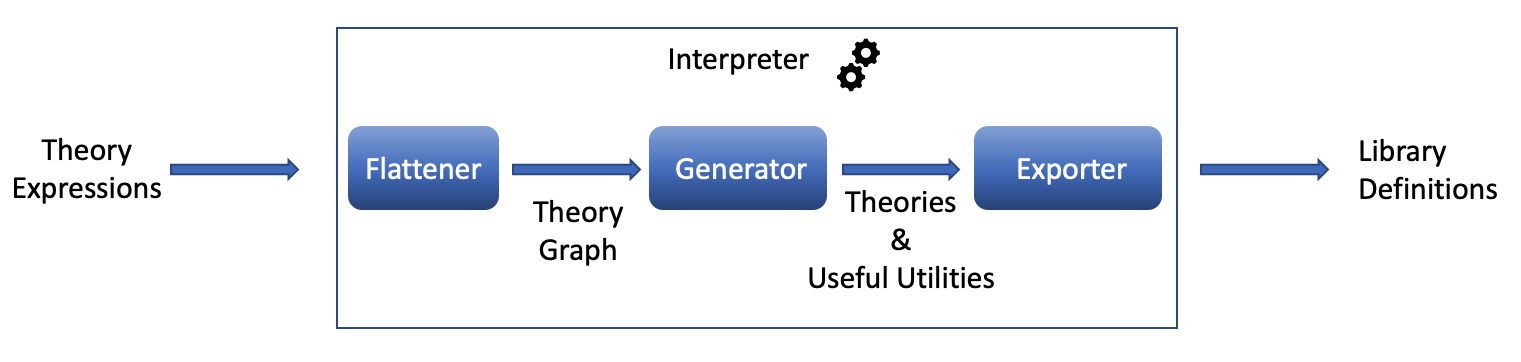
\includegraphics[scale=0.5,width=\linewidth]{figures/interpreter_detailed}
\caption{A $3$-staged interpreter for generating libraries}
\label{fig:staged-interpreter}
\end{figure}

\paragraph{Flattener.} The first stage of the interpreter builds a theory graph of algebraic structures. To provide more conciseness and better reuse, we use combinators to define new theories. The flattener uses expressions built using the combinators to build a theory graph. The problem here is to choose combinators that leverages the mathematical structure by providing expressive morphisms capable of describing the relationship between theories. We discuss our choice of combinators in Chapter~\ref{ch:library}. A strong requirement that we have regarding combinators is to allow computing flattened theories. While it is useful for the system to know that a \lstmath{Group} is a \lstmath{Monoid} with inverse and automate the transportation of theorems proved in \lstmath{Monoid} theory to be used in \lstmath{Group} theory, some potential users might want to use \lstmath{Group}s without caring about how they are built. We want to use combinators that allows both views for users, by avoiding qualified names and dropping and freeness combinators.\ednote{probably need references here.}
%without imposing one of Our library need to support both definitions, by enabling the users to work with flat version of the library. Some operations on theories make this hard to achieve, like dropping and freeness combinators by CASL\ednote{look for a source explaining why they are problematic}. 

\paragraph{Generator.} The input to the generator is a flat theory presentation, the output of the flattener. The generator manipulates the components of a theory presentation generating related constructions based on how they are defined in universal algebra. Therefore, the input theory needs to fit in the universal algebra abstraction of a theory, being a first-order equational theory. Despite this limitation, the algebraic hierarchy until at least \lstmath{Ring}\ednote{or maybe more?} fits in this criteria. 
We discuss our implementation of the generator in Chapter~\ref{ch:generation}. 

\paragraph{Exporter.} The Flattener and Generator deal with \emph{raw} mathematical definition, keeping system-specific design decision to a minimal. The exporter puts back these decisions. This way we provide customized definitions which increases their usability across different systems, users, and projects. \ednote{add reference to the chapter}. 




\chapter{Library}
\label{ch:library}
\ednote{for implementation of rename: check this:  Scrap Your Boilerplate: A Practical Design Pattern for Generic Programming} 

%One can define a new theory either by stating its components or by using combinators to build it from existing ones. 

In this Chapter, we build a library of axiomatic theories representing the algebraic hierarchy, before we use it to generate related constructions that we discuss in Chapter~\ref{ch:generation}. 

Our library consists of equational first-order theories organized as a theory graph using the tiny theories approach. Instead of having to provide all declaration of the theories and morphisms within the graph, we use the MathScheme combinators introduced in~\cite{CaretteOConnorTPC, carette2018building}. 

In Section~\ref{sec:background:tinytheories} we discuss tiny theories and present an example of building the theory of \lstmath{Unital} by extending the theory of \lstmath{PointedMagma} to create \lstmath{LeftUnital} and \lstmath{RightUnital}, then combining them. This example is described by the following diagram. \\
\begin{tikzcd}
& \verb|LeftUnital| \arrow[dr,hook] & \\
\verb|PointedMagma| \arrow[ur,hook] \arrow [dr,hook] & & \verb|Unital| \\
& \verb|RightUnital| \arrow[ur,hook] &
\end{tikzcd}
Whilte it is common to see the algebraic hierarchy as a series of inclusions as in Figure~\ref{fig:flatExtensions}, it really is more packed with diamonds, as in Figure~\ref{fig:cube_monoid}. 
\begin{figure}
\lstmath{Magma $\;\to\;$ Semigroup $\;\to\;$ Monoid $\;\to\;$ Group $\;\to\;$ $\cdots$}.
\caption{Algebraic structures as extensions}
\label{fig:flatExtensions}
\end{figure}  
%examining the work in \cite{halleck} and \cite{jipsen} show us that the algebraic %hierarchy is more packed with diamonds, as we show in Figure~


%\begin{figure}[h]
	\begin{tikzcd}[row sep=huge, column sep=scriptsize]
		&& & \verb|Pointed0| \arrow[dd,hook] & \\
		\verb|Carrier| \arrow[dd,hook] \arrow[rr,hook] & & \verb|Pointed| \arrow[ur,mapsto] & & \\ 
		& \verb|AddMagma| \arrow[rr,hook] \arrow[dd,hook]& & \verb|AddPointedMagma| 
		\arrow[rr,hook] 
		\arrow[dd,hook]& & 
		\verb|AddRightUnital|  \arrow[dd,hook]\\
		\verb|Magma| \arrow[ur,mapsto] \arrow[dd,hook]  & & 
		\verb|PointedMagma| \arrow[dd,hook] \arrow[ur,mapsto] \arrow[from=uu, crossing over] 
		\arrow[rr,hook,crossing over] \arrow[from=ll,hook, crossing over]
		& & \verb|RightUnital| \arrow[ur,mapsto] \\ 
		& \verb|AddSemigroup| \arrow[ddd,hook] & &\verb|AddLeftUnital| \arrow[rr,hook] &  & 
		\verb|AddUnital| \arrow[dddllll,hook] \\
		\verb|Semigroup|  \arrow[ddd,hook] \arrow[ur,mapsto]&  & \verb|LeftUnital| 
		\arrow[ur,mapsto] 
		\arrow[rr,hook,crossing over] &  & \verb|Unital| \arrow[dddllll,hook,crossing 
		over]\arrow[ur,mapsto] 
		\arrow[from=uu,hook,crossing over]& \\ 
		&&&& \\ 
		&  \verb|AddMonoid| &  &&\\ 
	 \verb|Monoid|  \arrow[ur,mapsto] && &&
	\end{tikzcd}
	\caption{Defining Monoid using tiny theories}
	\label{fig:cube_monoid}
%\end{figure}	
.
%As we discussed in Section~\ref{sec:thry_graph_in_action}, dealing with diamonds is a challenging problem~\cite{sakkinen1989disciplined, jigsaw1992, traits2006, diamonds2011}. There is a gap in how specification systems handle them, whether by not following its correct semantics, or by not supporting it at all. 

Diamonds are useful to capture the structure of mathematics, but they do not come without problems. We need to have careful infrastructure to deal with them in order to avoid the diamond problem~\cite{jigsaw1992,traits2006,diamonds2011}, a.k.a multiple inheritance or the fork-join problem~\cite{sakkinen1989disciplined}. 

In Section~\ref{sec:thry_graph_in_action} we provide an overview of the support for morphisms in different formal systems. Section~\ref{sec:msCombinators} introduces the MathScheme combinators which creates a morphism-based approach to building theory graphs, leading to a solution for the diamond problem. We discuss our implementation of the combinators  and the process of using them in library building in Section~\ref{sec:lib_implementation}\ednote{maybe split this section}. We recommend some guidelines for library building in Section~\ref{sec:guidelines} followed by some use cases that present useful insights. 
\ednote{give the overview of the sections}

\begin{comment}
To test our generation algorithms, we needed a large library of equational theories. As we have discussed in Section~\ref{sec:broader_context}, we work in the favor of a library organized as a theory graph, believing that it leverages the structure of mathematical knowledge. Arrows of the graph are the means to relating the different theories. In this section, we present our approach to building a library that emphasizes these connections. 

In Section~\ref{sec:thry_based_libs} we discuss the motivation behind building such a library. In Section~\ref{sec:ms_combinators} we present the combinators used in building it and discuss how they are arrow based. Section~\ref{sec:lib_implementation}, discusses the challenges of the implementation of the combinators to build a theory graph. We finally show some interesting cases of library definitions in Section~\ref{sec:interesting_cases}. 
\end{comment}


\section{Theory Graph Development}
\label{sec:thry_graph_in_action}

Although many formal systems support theory graph structure, the support they provide for arrows does not release its full power. 
Specware and MMT forces users to provide all details of theories and morphisms between them. IMPS generate morphisms given source and target theories. Clear

%On the other hand, it leads to a multiple diamonds (a.k.a. multiple inheritance) in the development of the hierarchy. 
%Many formal systems support a theory graph approach, and realizes the need of having morphisms between theories. Examples of these are Clear, OBJ, CASL, Maude, Specware, IMPS, and MMT. 

%Clear is - to our knowledge - the first system that provides a modular way to write formal specifications. It provide theory combinators to build larger theories from smaller ones. 
%\ednote{A good resource for Clear is the PhD thesis of Sanella with the title: semantics, implementation and pragmatics of CLEAR} 
Another way to support building a library rich in morphisms is to provide combinators to handle some of the work. Clear is - to our knowledge - the first system to use combinators for creating new theories\footnote{Clear is a specification language, and theories are used under the name specifications.}. OBJ and CASL are successors of Clear that also support combinators. We focus our discussion on CASL as a representative to this system, as it is the only living one now and so we were only able to look at its library and run experiments on it. 
We realize two problems related to combinators in CASL. First, It is not always possible to flatten theories build through the use of combinators, mainly when using hiding and freeness combinators~\cite{CoFI:2004:CASL-RM}. The second problem is related to how the \emph{union} operation is implemented. The \lstmath{union} operator is the one that handles multiple inheritance. Although the semantics of union is a pushout in the category of specifications and morphisms, it is computed on a 'same name, same thing' basis~\cite{bidoit2003casl}. Figure~\ref{fig:casl_expr} shows the problems that occur from using this principle. 
\begin{figure}
\begin{tikzpicture}[node distance=2cm]
    \node(NodeName1){
\begin{tcolorbox}[colback=white, width= 0.45\textwidth,left=0pt,right=0pt,top=0pt,bottom=0pt]
\begin{caslcode}
spec BaseSpec = sort A end 
spec Ext1 = BaseSpec then 
 ops e  :A 
   __*__:A * A -> A,unit e 
end 
spec Ext2 = BaseSpec then 
 ops e :A 
   __+__:A * A -> A, unit e 
end 
spec Combine = 
   Ext1 and Ext2 
end
\end{caslcode}   
\end{tcolorbox}
    };
\node(NodeName2) [right=of NodeName1] {  % added position of second box
    \begin{tcolorbox}[colback=white, width= 0.45\textwidth,left=0pt,right=0pt,top=0pt,bottom=0pt]
\begin{caslcode}
  sorts A
  op __*__ : A * A -> A
  op __+__ : A * A -> A
  op e : A
  forall x : A . x + e = x 
   %(ga_right_unit___+__)%
  forall x : A . e + x = x 
   %(ga_left_unit___+__)%
  forall x : A . x * e = x 
   %(ga_right_unit___*__)%
  forall x : A . e * x = x 
   %(ga_left_unit___*__)%
\end{caslcode} 
        \end{tcolorbox}
        };
\draw[black, line width=2mm,-{Triangle[angle=60:1pt 3]}] (NodeName1) -- (NodeName2);
\end{tikzpicture}
\caption{CASL union operation: On the left, the specification \lstinline|Combine| is defined as the union of \lstinline|Ext1| and \lstinline|Ext2|. On the right, the declarations of specification 
\lstinline|Combine| as computed by CASL.}
\label{fig:casl_expr}
\end{figure}
Both specifications \verb|Ext1| and \verb|Ext2|, on the left side, extend the \verb|BaseSpec| with a binary operation and its unit element. In case of \verb|Ext1|. A pushout between the two arrows \lstmath{BaseSpec $\;\to\;$ Ext1} and \lstmath{BaseSpec $\;\to\;$ Ext2} would result in a theory with one sort \lstmath{A},and  two binary operations with two different unit elements. When trying this specification in CASL\footnote{using the online tool at: \url{http://rest.hets.eu}}, it computes the declarations on the right side of the figure which has only one unit element for the two binary operations. This is different from what a pushout would compute. 

We performed the same experiment with Isabelle locale expressions~\cite{ballarin2003locales} and got similar results. In the following section, we introduce a collection of combinators that provide solid infrastructure for dealing with theories and morphisms to build a large library organized as a theory graph. 

\section{MathScheme Combinators}
\label{sec:msCombinators}

Combinators provide algebra for manipulating theories in different ways. They enhance modularity, reusability and maintainability of the library by saving the user the need to repeat definitions. \cite{carette2018building} introduces $4$ combinators based on the definitions of theories as contexts, and theory morphisms in dependent type theory as we discuss them in Sections~\ref{sec:background:theory} and \ref{sec:background:morphisms}. %The combinators form a language to create a librarnew theories by reusing older ones. We use this language to build a library of $250$ theories as we discuss in Section~\ref{sec:lib_implementation}. 
%many theorem provers that are in use today, do not have the notion of morphism and suffer from redundancy. Agda and Coq are big examples of that. Apart from extensions, they do not support combining modules.

%In~\cite{carette2018building}, we present $4$ combinators along with their operational and categorical semantics. The semantics we provide is based on the category of contexts and the categorical semantics of dependent type theory. In the following section we present the combinators and their semantics. 

%Despite the large literature on using combinators to save work and reduce redundancy, Most of the systems we listed here suffer from redundancies in their own libraries. \ednote{Add an appendix about the different redundancies}To avoid this redundancy, we suggest in~\cite{carette2018building} a set of combinators that form a compact language to describe algebraic theories by reusing older ones. We use these combinators to build our library as well as some important design decisions 
A library built using these $4$ combinators respect the following design decisions 
\begin{itemize}
    \item Theories can always be flattened. Not all users of a formal system are interested in the hierarchy used to build the theories their need. A mathematician who wants to prove results in \verb|Group| theory is only interested in groups with their standard definitions and results. This user should not be forced to work with groups as extensions of some theory, like \verb|Monoid|. Abstracting over the hierarchy in users' code also has the advantage that the code need not change in case the hierarchy change, like what happened in the case of changing the type class hierarchy in Haskell~\cite{wiki:haskell_hierarch}. 
    \item Names are taken seriously. Similar concepts have different names in different contexts of mathematics. The unit of \verb|_+_| has a different name than the one of \verb|_*_| and confusing their names would be a huge usability problem. The combinators introduced in~\cite{carette2018building} does not generate any names nor attempt to use any heuristics to solve name clashes. Instead name clashes are detected and the library developer is asked to resolve them.  
    \item Tiny theories are systematically used. Since we do not provide a drop combinator, we use tiny theories to make sure all intermediate results are available for future theories to use. 
    \item Arrows are the main building unit of the library. The semantics and the implementation of the combinators is based on arrows, not theories. This makes it possible compute category theory operations based on their real semantics, not an approximation like same-name-same-thing. 
\end{itemize}


The combinators assume theories expressed in an underlying dependent type logic. Therefore, a theory is viewed as a context, or a telescope as defined in equation~\ref{eq:telescope}. The combinators uses DTT as their foundation, but abstracts on many of the details of the type theory. The minimum requirements of the underlying logic are listed in ~\cite{carette2018building}. We include them here for coherence. These requirements are 
\begin{itemize}
    \item An infinite set of variable names \vars.
    
    \item A typing judgement for terms $s$ of type $\sigma$ in a context
    $\Gamma$ which we write $\Gamma \vdash s : \sigma$.
    
    \item A kinding judgement for types $\sigma$ of kind $\kappa$ in a context
    $\context{\Gamma}$ which we write\\
    $\context{\Gamma} \vdash \sigma : \kappa : \Box$.  We further assume that the set
    of valid kinds $\kappa : \Box$ is given and fixed.
    
    \item A definitional equality (a.k.a. convertibility) judgement of terms
    $s_1$ of type $\sigma_1$ and $s_2$ of type $\sigma_2$ in a context $\context{\Gamma}$,
    which we write $\context{\Gamma} \vdash s_1 : \sigma_1 \equiv s_2 : \sigma_2$. \ We
    will write $\context{\Gamma} \vdash s_1 \equiv s_2 : \sigma$ to denote $\context{\Gamma} \vdash
    s_1 : \sigma \equiv s_2 : \sigma$.
    
    \item A notion of substitution on terms. Given a list of variable
    assignments $\assignment{x_i}{s_i}{i < n}$
    and an expression $e$ we write $\substitutiondef{e}{x_i}{s_i}{i < n}$
    for the term $e$ after simultaneous substitution of variables $\left\{ x_i
    \right\}_{i < n}$ by the corresponding term in the assignment.
\end{itemize}

The $4$ combinators in~\cite{carette2018building} are: 
\subsection{Extension} 
\label{subsec:extension}
Extensions are the most basic combinator. On its own, it makes it possible to define a flat hierarchy as in Figure~\ref{fig:flatExtensions}. 

The input to an extension combinator are a theory presentation $\Gamma$ and a list of declarations $\extDecls = \left\{a_{i}:\sigma_{i}:\kappa_{i}\right\}_{i<n}$. 
The combinator computes a new theory (\lstmath{pres}) $\Gamma\rtimes\Delta^+$ and an identity morphism (\lstmath{$\tilde{\text{id}}$}) from $\Gamma$ to $\Gamma\rtimes\Delta^+$, where $\rtimes$ is asymmetric operation that adds definitions to a telescope. On one side $\Gamma$ is a well-formed theory, but $\Delta^+$ may not be well-formed on its own. 
The construction is defined as
\[\extensionDef{\extSource}{\extDecls}\]

$\Delta^+$ is a sequence of declarations $\{a_i : \sigma_i : \kappa_{i}\}$. An extension is well-formed if 
\begin{eqnarray}
\forall i \cdot a_i \notin \syms{\Gamma_{i-1}} \\
\forall i \cdot \Gamma_{i-1} \vdash \sigma_i : \kappa_{i}
\end{eqnarray}
where $\Gamma_{i-1} = \Gamma \rtimes \{a_0 : \sigma_0 : \kappa_0\  \cdots \ a_{i-1} : \sigma_{i-1} : \kappa_{i-1}\}$ 

%\paragraph{Categorical Semantics}
%In the category of contexts $\ctxcat$, an extension corresponds to a forgetful functor. 

\paragraph{Example}
Extensions are used when new concepts are added. According to little theories, the concept need to be added in its smallest context, i.e. if $\Gamma \vdash c : t$ then for every $\Sigma \subset \Gamma$, $\Sigma \nvdash c : t$. Tiny theories encourages adding one new declaration at a time. A good example is adding properties of a binary operation, like \lstmath{commutativity} or \lstmath{associativity} as follows\footnote{The syntax we use here is the one used in our implementation. It is clear enough to be understood without problems.} 
\begin{togcode}
Semigroup = extend Magma {assoc : { x y z : A } ~$\to$~ op x (op y z) ==
                                                   op (op x y) z } 
CommMagma = extend Magma {comm  : { x y : A } ~$\to$~ op x y == op y x }
\end{togcode} 
where \lstmath{Magma} is the theory $\Gamma$ being extended, \lstmath{assoc} and {comm} are definitions in $\Delta^+$. 

\subsection{Rename}
\label{subsec:rename}
Renames do not add new concepts, but allows using flexible notations while still reusing all results from the source theory. 
Given a theory presentation $\Gamma$ and a rename function $\pi$, the output of the rename operation is a new theory (\lstmath{pres}) $\pi \cdot \Gamma$ which is computed by performing a substitution of $\pi$ into the declarations of $\Gamma$, and an embedding morphism $\tilde{\pi} : \Gamma \to \pi\cdot\Gamma$ that maps symbols of $\Gamma$ to those of $\pi\cdot\Gamma$ based on the renaming function $\pi$. 
\[ \renameDef{\renSource}{\renFun} \]

A rename operation is well-formed whenever the rename function $\pi : |\Gamma| \to \vars$ is a injection, and the codomain is a $k-$permuation on $\vars$, where $k$ is the number of declarations in $\Gamma$. 

\paragraph{Example}
After defining \lstmath{Semigroup} in the example of the previous section over a binary operation \lstmath{op}, one would want to define the additive and multiplicative versions using the symbols \lstmath{+} and \lstmath{*}, resp. It also make sense to have a morphism from \lstmath{Semigroup} to those variants that only differ in the names of the symbols. The rename combinator does just that 
\begin{togcode}
AddSemigroup  = rename Semigroup {op to +} 
MultSemigroup = rename Semigroup {op to *} 
\end{togcode}  

\subsection{Combine}
\label{subsec:combine}
Conisder the following small library
\begin{togcode} 
Theory Empty = {} 
Carrier = extend Empty {A : Set}
Pointed = extend Carrier {e : A}
Magma   = extend Carrier {op : A -> A -> A}
\end{togcode} 
The flattened version of the theories of these libraries are 
\begin{itemize}
\item[] \lstmath{Carrier = [A : Set]}
\item[] \lstmath{Magma = [A : Set, op : A $\;\to\;$ A $\;\to\;$ A]} 
\item[] \lstmath{Pointed = [A : Set, e : A]} 
\end{itemize}
Now we want to define the theory \lstmath{PointedMagma} which has a binary operation and a point. It makes sense to assume this theory to be an extension of both \lstmath{Magma} and \lstmath{Pointed}. Using the extension combinator will not help us here. In this situation, we are facing the diamond problem in which our new theory is inheriting from two theories and it is not clear whether a declaration, lilke \lstmath{A : Set} should be repeated or not. 
The situation is more complicated if we consider the following definition of \lstmath{AddSemigroup} by relating it to \lstmath{AddMagma} defined as 
\begin{togcode} 
AddMagma = rename Magma {op to +} 
\end{togcode} 
and \lstmath{Semigroup} defined as in Section~\ref{subsec:extension}. Here we have the same binary operation with different names. Which name should be used? Or should they be repeated, having two  binary operations in the outcome? 

The case when a theory needs to be related to more than one is prevalent when building large libraries. As we see in these examples, it occurs very early on when formalizing the algebraic hierarchy. The combine operation supports the multiple inheritance situation by relying on the information in the morphisms. Combine performs a pushout of the morphisms in the category of theory presentations, i.e. a pullback in the category of contexts.  A pushout is a $5-$ary operation that takes $2$ arrows and $3$ objects of a category. The arrows need to originate from the same source. The $3$ theories can be deduced from the arrows as the two target theories of the arrows and their common source. For cases where there are name clashes, like the name clash between \lstmath{op} and \lstmath{+} in the \lstmath{AddSemigroup} example, the user is required to provide renames in case of this clash. This is consistent with our design decision to not use heuristics or name generation to resolve any name conflists. 

The combine operation between two morphisms is defined as $u_{\Delta}$ and $u_{\Phi}$ both having $\Gamma$ as their source, and having $\Delta$ and $\Phi$, resp, as their targets. 
\[
\comfun\left( u_{\Delta}, u_{\Phi}, \pi_{\Delta}, \pi_{\Phi}\right) \define
\left\{\begin{aligned}
\mathtt{pres} & = \combineResult_0\rtimes\left(\combineResult_{\Delta} \cup \combineResult_{\Phi}\right) \\
\mathtt{embed}_{\Delta} & = \left[v_{\Delta}\right] : \Delta\rightarrow\combineResult\\
\mathtt{embed}_{\Phi} & = \left[v_{\Phi}\right] : \Phi\rightarrow\combineResult\\
\mathtt{diag} & = \left[uv\right]:\Gamma\rightarrow\combineResult\\
\end{aligned}\right\}\]
% ----------------- the removed mediate ----------------- 
% \mathtt{mediate} & = \lambda\ w_{\Delta}\ w_{\Phi}\ .\  w_{\combineResult}
% --------------------------------------------------------
 
%To say a \lstmath{Monoid} is a \lstmath{Semigroup} and a \lstmath{Unital}, we need multiple inheritance, which creates a diamond structure. The \lstmath{Combine} operation is the one to use in this case. 
%It is well agreed upon that the semantics of such an operation should be a pushout in the category of theory presentations\ednote{cite the other systems or refer to a previous section}.
where $\pi_{\Delta}$ and $\pi_{\Phi}$ are two rename functions given to resolve name conflicts. 

There is the following precondition for performing a combine 
\begin{equation}
\pi_{\Delta} \left( x \right) = \pi_{\Phi} \left( y \right)
\Leftrightarrow \exists z \in \left| \Gamma \right|.\ x =
\substitution{z}{u_{\Delta}}{} \wedge y = \substitution{z}{u_{\Phi}}{} 
\label{eq:combinePrecond}
\end{equation}
where \lstmath{x $\;\in$ $\mid\Delta\mid$} and \lstmath{y $\;\in$ $\mid\Phi\mid$}. 
This precondition ensures that after applying the rename function on symbols \lstmath{x} and \lstmath{y}, if they map to the same symbol then they have originated from the same symbol in the source theory $\Gamma$. It also ensures that there are no name clashes when mapping a symbol $z$ across the two morphisms and rename functions.  

\paragraph{Example}
We have given two examples in the beginning of this section illustrating situations in which combine operations is needed. A \lstmath{PointedMagma} is defined as 
\begin{togcode} 
PointedMagma = combine Magma {} Pointed {} 
\end{togcode} 
The embeddings being combined are \lstmath{Carrier $\;\hookrightarrow\;$ Magma} and \lstmath{Carrier $\;\hookrightarrow\;$ Pointed}. The empty 
\lstinline|{}| means the identity rename functions are used in this expression, as in this case no name clashes need to be resolved. 

The \lstmath{AddSemigroup} is defined as 
\begin{togcode} 
AddSemigroup = combine AddMagma {} Semigroup {op to +} 
\end{togcode} 
The embeddings used here are \lstmath{Magma $\;\mapsto\;$ AddMagma} and \lstmath{Magma $\;\hookrightarrow\;$ Semigroup}. The declaration \lstmath{op} in \lstmath{Magma} is mapped to \lstmath{+} in \lstmath{AddMagma} and remains as \lstmath{op} in \lstmath{Semigroup}. Therefore, a rename \lstinline|{op to +}| is needed to resolve this name clash. 
%The work in \cite{carette2018building} defines $4$ combinators used to build a graph of axiomatic theories in a dependently-typed logic. This graph corresponds to a diagram in the category $\tpcat$ of theory presentations and morphisms between them.
%    \item The category of contexts $\ctxcat$ is the opposite of the category of theory presentations $\tpcatOp$, i.e. if a theory \lstmath{T'} is the extension of a theory \lstmath{T} in the category $\tpcat$, then there is a morphism in $\ctxcat$ from \lstmath{T'} to \lstmath{T} that drops some of the declarations in \lstmath{T}. Because theories are viewed as telescopes, to drop a declaration, all its subsequent ones need to be dropped. 
 %   \item A fibered category is \ednote{short description here}. The category of context $\ctxcat$ forms the basis of a fibration, with the fibered category being the category of extensions $\extcat$. The fibration maps every extension object from $\extcat$ to its source in $\ctxcat$. 

\subsection{Mixin}\ednote{@JC: Can you please check this section more thoroughly. I am not sure I fully understand mixins}
\label{subsec:mixin}
The combinators we have presented so far deal with embeddings. A general morphism, as discussed in Section~\ref{sec:generalmorph}, is not supported by any of them. The mixin combinator computes pushout of an embedding along a general morphism. Given a general morphism \lstmath{$[\text{u}_\Delta]: \Gamma \to \Delta$} and an embedding \lstmath{$[\text{u}_\Phi] : \Gamma \to \Phi$} and two injective renaming functions 
\lstmath{$\pi_\Delta : \mid\Delta\mid \to \mathbb{V}$}
and \lstmath{$\pi_\Phi : \mid\Phi\mid \to \mathbb{V}$}, the mixin is defined as follows 
\[
\mixfun\left( u_{\Delta}, u_{\Phi}, \pi_{\Delta}, \pi_{\Phi}\right) \define
\left\{\begin{aligned}
  \mathtt{pres} & = \combineResult_1\rtimes\combineResult_2 \\
  \mathtt{embed}_{\Delta} & = \left[v_{\Delta}\right] : \Delta\rightarrow\combineResult\\
  \mathtt{view}_{\Phi} & = \left[v_{\Phi}\right] : \Phi\rightarrow\combineResult\\
  \mathtt{diag} & = \left[uv\right]:\Gamma\rightarrow\combineResult\\
\end{aligned}\right\}
\]
%  \mathtt{mediate} & = \lambda\ w_{\Delta}\ w_{\Phi}\ .\  w_{\combineResult}
where $\Xi_1 = \pi_\Delta \cdot \Delta$ is the theory presentation resulting from applying the rename function $\pi_\Delta$ to $\Delta$ via substitution. 
$\Xi_2 = \pi_\Phi \cdot \Phi^+$ is not a well-formed theory presentation, instead, it is the result of applying $\pi_\Phi$ to declarations of $\Phi$ that are not mappings of declarations in $\Gamma$. 
In~\cite{carette2018building}, proofs that the mixin operation as described above is always well-formed has been presented. 

\paragraph{Example} In Section~\ref{sec:generalmorph} we introduced the \lstmath{flip : Magma $\;\to\;$ FlippedMagma} morphism. The following expression, we use it to construct flipped \lstmath{Semigroup}
\begin{togcode} 
FlippedSemigroup = mixin flip {} Semigroup {} 
\end{togcode} 
In this case, $\text{u}_\Delta$ is the \lstmath{flip} morphism, $\text{u}_\Phi$ is the morphism \lstmath{Magma $\;\to\;$ Semigroup}. Therefore, the resulting presentation \lstmath{pres} will have definitions from \lstmath{FlippedMagma} and the associativity axiom from \lstmath{Semigroup}. 

\section{Combinators Implementation}
\label{sec:lib_implementation}
The combinators from~\cite{carette2018building} has been implemented in~\cite{cicm2019diagrams, TPCProto, meta-prim-blog}. Experiments have been performed on applying them for creating a large library of algebraic constructions~\cite{mathscheme2011experiments}. With the exception of~\cite{cicm2019diagrams}, the other implementations and the associated library did not emphasize the morphisms in the way presented in~\cite{carette2018building} and summarized in the previous section. Instead, they based their computation of pushout on theories using same-name-same-thing approach, which makes errors like the one in Figure~\ref{fig:casl_expr} go undetected.  
This approach also computes results for expressions that should not be meaningful in the language of combinators presented in~\cite{carette2018building}. Consider the following expression
\begin{togcode}
SemiRng = combine AdditiveCommutativeMonoid Semigroup Ringoid
          over RingoidSig
\end{togcode}
Note that the definition of \lstmath{SemiRng} above is different from the syntax we presented before. First, there is no mention of the rename function, as they all are the identity. Second, there are $3$ theories being combined. Normally, we talk about combining $2$ arrows with the semantics being the pushout. In this case, we have $3$ arrows each has the source \lstmath{RingoidSig} and the three targets are the arguments to combine. In this case, we are computing colimits, not pushouts. Finally, there is the \lstmath{over} part of the expression which was part of the original work in~\cite{CaretteOConnorTPC} and then removed in the more recent version~\cite{carette2018building}. The over part specifies what the source of the morphisms is. In Section~\ref{subsec:overPart} we discuss why we need an \lstmath{over} part in the combine declaration. 

An implementation that reflects the principles of the combinators will not be able to find a morphism between \lstmath{RingoidSig} (the common source) and \lstmath{Semigroup} (the second target). 
The theory \lstmath{RingoidSig} has declarations for two binary operations, while \lstmath{Semigroup} has only one. A morphism from \lstmath{RingoidSig} to \lstmath{Semigroup} needs to drop one binary operation. This is not possible given the choice of combinators that avoids a drop operation. 

In Section~\ref{subsec:coreDecisions} we discuss the main design decisions that we take on top of those in~\cite{carette2018building}. We start discussing our implementation in Section~\ref{subsec:theoriesMorphisms} by presenting how we represent theories and morphisms in our framework. In Section~\ref{subsec:graph} we present the type of the theory graph. The implementation of the combinators that build the graph is presented in Section~\ref{subsec:combinatorsImpl}. 

\subsection{Core Design Decisions}
\label{subsec:coreDecisions}
We build our implementation on two main design decisions that restrict the original combinators to solve some implementation issues. We conclude by summarizing the syntax of the tog expressions that we use based on the syntax of the combinators. 
\subsubsection{Referring to arrows}
\label{subsec:overPart}
The extension and rename combinators needs to identify a theory in the graph to operate on and compute the output theory and arrow. The input theory is part of the expression of the combinator. 
In the case of \lstmath{combine}, the inputs to the combinator are two morphisms and two rename functions. But the syntax for combine is not defined in terms of arrows. Instead, it is defined in terms of theories and the arrows are left to the implementation to infer them. 
For example, the expression 
\begin{togcode}
combine CommutativeMagma {} AssociativeMagma {}
\end{togcode}
does give information that the targets of the two embeddings involved are \lstmath{CommutativeMagma} and \lstmath{AssociativeMagma}, but it does not specify the source of the embeddings. The algorithm has three choices of the source theory, which is common to both morphisms. 
\begin{itemize}
    \item If the source theory is \lstmath{Magma}, the theory resulting from the combine operation will have one binary operation that is both associative and commutative 
    \item If the source theory is \lstmath{Carrier}, then the definition is describing a theory (along with the related morphisms) that has two binary operations, one associative and the other commutative. But this theory will not be computed because of the name clash; The user has to choose another name for one of the two operations. A possible fix is 
    \begin{togcode}
combine CommutativeMagma {op to +} AssociativeMagma {op to *}
    \end{togcode}
\end{itemize}
As the hierarchy gets deeper this problem becomes more complicated. For example, \lstmath{CommutativeGroup} and \lstmath{AssociativeGroup} have many more possibilities for their common source. 

The reason of this problem is that the syntax of the language presented in~\cite{carette2018building} is based on naming target theories, while the syntax is based on having the embedding available. This leaves the gap of using the target theories to infer the embeddings. Using theories, instead of morphisms, in the syntax is a usability decision. Arrows do not have canonical names, mainly because they do not appear in informal mathematics. For example, it is hard to think of a name for the arrow (the result of composition of arrows) from the \lstmath{PointedMagma} to \lstmath{Monoid} theory. It is easier to refer to it in terms of the source and the target than to give it any name. 

We use an approach that still uses theories for usability reasons but gives more information for inferring the embeddings. We modify the syntax of \lstmath{combine} in the paper to have an \lstmath{over} part similar to the initial work on the combinators~\cite{CaretteOConnorTPC}. 

\subsubsection{All Paths Commute Approach} 
\ednote{@JC: Do we need to remove mixin, so all paths commute?} 
When referring to an arrow using its source and target, we implicitly assume that all paths commute, i.e.: Given the source and target, they either is no path, one path, or multiple paths that commute between them. 

In Section~\ref{sec:background:morphisms}, we discussed the three types of arrows, identity, embeddings and general morphisms. We also noted in Section~\ref{subsec:mixin} that the only combinator that accepts and generates a general morphism is \lstmath{mixin}. If we restrict our language to \lstmath{extension}, \lstmath{rename}, and \lstmath{combine}, we end up with an all-embeddings graph, in which all paths commute. 

\subsubsection{Theory Expressions}
\label{sec:impl:expressions}
The language that we implement has the following syntax
\begin{togcode}
 Map m = {a~$_0$~ to b~$_0$~ ; ~$\cdots$~ ; a~$_n$~ to b~$_n$~}
 Theory T = {a~$_0$~ : t~$_0$~ ~$\cdots$~ a~$_n$~ : t~$_n$~}
 extend T {a~$_0$~ : t~$_0$~ ~$\cdots$~ a~$_n$~ : t~$_n$~}
 rename T m 
 combine T~$_1$~ m~$_1$~ T~$_2$~ m~$_2$~ over T
 id from T~$_1$~ to T~$_2$~
\end{togcode} 
%{a~$_0$~ to b~$_0$~ ; ~$\cdots$~ ; a~$_n$~ to b~$_n$~}
%{a'~$_0$~ to b'~$_0$~ ; ~$\cdots$~ ; a'~$_n$~ to b'~$_n$~}
where \lstmath{T}, \lstmath{T$_1$}, and \lstmath{T$_2$} are theories, \lstmath{m}, \lstmath{m$_1$}, and \lstmath{m$_2$} are mappings that are either previously defined using the \lstmath{Map} keyword or expanded as a list of mappings 
\lstmath{$\{$a$_0$ to b$_0$ ; ... ; a$_n$ to b$_n$ $\}$}. 

Although one can declare a theory with a list of declarations using the \lstmath{Theory} keyword, we only use it to create the empty theory. 


\subsection{Theories and Morphisms}
\label{subsec:theoriesMorphisms}
We defined a theory in DTT in Section~\ref{sec:background:theory} as a telescope.  Itis captured by the type \lstmath{GTheory}. 
\begin{hscode}
data GTheory = GTheory {
  declarations :: [Constr],
  waist        :: Int     }
\end{hscode}
The waist is needed to determine how many of the declarations are parameters, as in~\cite{alhassy2019}. 

The type \lstmath{GView} describe the morphism as defined in~\ref{sec:background:morphisms}. 
\begin{hscode}
data GView  = GView {
  source  :: GTheory,
  target  :: GTheory,
  rename :: Rename }  
\end{hscode}
where \lstmath{type Rename = Map.Map Name_ Name_} is the mapping function. 

\subsection{Theory Graph Structure}
\label{subsec:graph}
We define a theory graph as a name-to-theory map and a name-to-view map 
\begin{hscode}{haskell}
data TGraph = TGraph { 
  _nodes :: Map.Map Name_ GTheory,
  _edges :: Map.Map Name_ GView } 
\end{hscode}
An alternative way to represent graphs would have been to include only the \lstmath{_edges}, as they contain information about theories. We preferred to keep both mappings to make it easier to lookup theories in the graph. 

We noticed that in many cases, the same renames are being reused. So, we also added a \lstmath{Mapping} type that allows the user to define something like 
\begin{hscode}
Map plus-zero = {op to + ; e to 0}
\end{hscode}
and reuse it. Accordingly, a library consists of a theory graph and some mappings. 
\begin{hscode}
data Library = Library {
  _graph   :: TGraph,
  _renames :: Map.Map Name_ Rename }
\end{hscode}

\subsection{Combinators}
\label{subsec:combinatorsImpl}
The language extension that we introduce to tog is described in the type \lstmath{Language} 
\begin{togcode}
data Language = 
    MappingC Name [RenPair]
  | TheoryC Name [Constr]
  | ModExprC Name ModExpr
\end{togcode}
where \lstmath{MappingC} creates a mapping function, \lstmath{TheoryC} creates a theory from a list of declarations, and \lstmath{ModExprC} is the constructor for creating theory expressions. We discuss them in the following sections. 

%We introduced the expressions we use to build the theory graph in Section~\ref{sec:impl:expressions}. In this section, we discuss our implementation for these expressions. The language that we introduce to Tog is described here 

\subsubsection{Mappings}
A definition of a mapping is elaborated into an entry in the \lstmath{renames} list of the library. 
\begin{hscode}
addMapping :: Name -> [RenPair] -> Library -> Library
addMapping nm rens = 
   over mappings (Map.insert (nm^.name) (renPairsToMapping rens))
\end{hscode}
\lstmath{over} is the setter function we get by using Haskell lenses. It sets the \lstmath{mappings} field of the library to a new instance of \lstmath{Map} that adds the new mapping to the ones in the input library. 

\subsubsection{Flat Theories}
Given a theory presentation as a list of declarations, we construct the new theory and add it to the list of theories in the graph without any morphisms connecting them to other theories. 
\begin{hscode}
theory :: Name -> [Abs.Constr] -> Library -> Library
theory nm cList =
  let newThry  = GTheory cList waistNm
  in  over graph (over nodes (Map.insert (nm^.name) newThry))
\end{hscode}


\subsubsection{Theory Expressions}
The syntac for the theory expression is introduced in Section~\ref{subsec:coreDecisions}. We now discuss their implementation. 
We start with the function \lstmath{updateGraph} which adds theories and morphisms to the graph, assuming they already have been computed by the combinator
\begin{hscode}
updateGraph ::   Name_ -> Either GView PushOut -> TGraph -> TGraph
updateGraph nm (Left view) =
  over nodes (Map.insert nm (target view)) .
  over edges (Map.insert ("To"++nm) view)
updateGraph nm (Right ut) =
  over nodes (Map.insert nm (target ~$\$$~ uLeft ut)) .
  over edges (\e -> foldr (uncurry Map.insert) e 
                        [("To"++nm++"1",uLeft ut),
                         ("To"++nm++"2",uRight ut),
                         ("To"++nm++"D",diagonal ut)])
\end{hscode}
The first argument to \lstmath{updateGraph} is the name of the new theory. Then, the function expects the arrows resulting from the combinator to be added to the graph. We know that all the combinators compute only one new theory. 
But, the number of computed arrows is different based on the combinators. \lstmath{extends} and \lstmath{rename} generates one morphism, while \lstmath{combine} generates three. We capture this with the type \lstmath{Either GView PushOut}, where \lstmath{Pushout} is defined as 
\begin{hscode}
data PushOut = PushOut { -- of a span
  uLeft    :: GView,
  uRight   :: GView,
  diagonal :: GView,
  apex     :: GTheory } -- common point
\end{hscode}
The names of the new arrows are generated based on the names of the new theories. Since a new theory with a user given name is defined every time, we know that the new arrow names have not been generated before. 

The functions \lstmath{computeExtend}, \lstmath{computeRename}, and \lstmath{computeCombine} calculate the new arrows and theories. 

\paragraph{1. Computing Extension}
The inputs to the extension operation is the theory being extended and the new declarations. The new theory is obtained by concatenating the new declarations to the ones already in the theory, given that there is no name clashes between new constructs, and that they are well-typed in the context presented by the theory declarations. 

The resulting view has the input theory as source, the computed theory as target. The identity mapping is computed using the \lstmath{validateRen} function, which assigns a mapping to every symbol in the input theory. In the case of extension the mapping is the identity. 
\begin{hscode}
computeExtend :: [Constr] -> GTheory -> GView
computeExtend newDecls srcThry =
  GView srcThry (extThry newDecls srcThry) (validateRen srcThry Map.empty)

extThry :: [Constr] -> GTheory -> GTheory 
extThry newConstrs thry@(GTheory constrs wst) =
  if List.intersect newConstrNames (symbols thry) == []
  then GTheory (constrs ++ newConstrs) wst
  else error ~$\$$~ "Cannot create theory "
    where newConstrNames = map getConstrName newConstrs
\end{hscode}

\paragraph{2. Computing Rename}
Computing renames requires computing substitutions. This requires traversing the internal representation of the theory and performing substitution as needed. We use Haskell's scrap-your-boilerplate package~\cite{syb}, based on~\cite{syb2003Jones}, to perform the traversal. The substitution is then performed using the \lstmath{gmap} function. 
\begin{hscode} 
gmap :: (Generics.Typeable a, Generics.Data b) => (a -> a) -> b -> b
gmap r x = Generics.everywhere (Generics.mkT r) x  
\end{hscode} 
\lstmath{gmap} traverses an instance of type \lstmath{b} changing every instance of \lstmath{a} according to the input function \lstmath{r}. \lstmath{computeRename} uses \lstmath{gmap} to perform substitution to declarations of the input theory, as follows
\begin{hscode}
computeRename :: Rename -> GTheory -> GView  
computeRename namesMap thry =
  GView thry (renameThy thry namesMap) (validateRen thry namesMap)

renameThy :: GTheory -> Rename -> GTheory
renameThy (GTheory constrs wst) m =
  GTheory (gmap (mapAsFunc m) constrs) wst
\end{hscode}

\paragraph{3. Computing Combine}
The algorithm to compute the result of combining two embeddings work as follows 
\begin{itemize}
    \item Given the name of the source theory and the two theories to be combined, the first step is to lookup the paths from the source to the target theory. A path is defined as a non-empty list of views. The function \lstmath{getPath} searches the graph for a path between given source and target theories. It starts at the target node and goes backwards, exploring the possible paths until it finds the source. Because none of the combinators result in backward arrows, we know the theory graph has no cycles, it actually looks more like a tree. Therefore, this simple search for a path algorithm works. The two paths are used to construct two instances of \lstmath{QPath}. 
\begin{hscode}
data QPath = QPath { 
  path :: Path,
  ren  :: Rename }
\end{hscode}

    \item At this point we have the two embedding and the two rename functions. The next step is to check the preconditions of \lstmath{combine} as in equation~\ref{eq:combinePrecond}. The function \lstmath{checkGuards} checks that all symbols in the source theory are mapped to the same symbol after applying the rename function. The scope checker of tog ensures the background direction of the equivalence in equation~\ref{eq:combinePrecond}. If the two instances of \lstmath{QPath} passes the precondition, the pushout can be computed.
    
    \item The result theory is computed by taking the disjoint union of the declarations in the source theory, the one on the left of the diamond (the first argument), then the one on the right. Note that this operation is not commutative. If we take the disjoint union of the source, right, then left theories, we get an equivalent but not equal theory. The order of declarations will be different, but the two theories will have the same declarations. 
\begin{hscode}
 newThry = 
   GTheory (disjointUnion3 (declarations srcMapped)
                           (declarations lThry) 
                           (declarations rThry)) 
           (waist srcMapped)
\end{hscode}    
    \item The source and target of the resulting morphisms are easy to figure out. The function \lstmath{allMaps} calculate the mappings by composing the mappings in the views on the path between the two theories, and then the one described by the rename function. 
\begin{hscode}
lView = GView lt newThry ~$\$$~ validateRen lt (allMaps left)
rView = GView rt newThry ~$\$$~ validateRen rt (allMaps right)
diag  = GView commonSrc newThry ~$\$$~ validateRen commonSrc (allMaps left)
\end{hscode}
\end{itemize}

\section{Library Building}
\label{sec:guidelines}
Once implementation of combinators is in place, we start using them to build the library organized as a theory graph. Our guide in building this library are the definitions in~\cite{msLibDecls}, which were part of an experiment~\cite{mathscheme2011experiments} on the way to develping the combinators we discuss in this chapter. Therefore, there are some definitions in that library that referred to non-existing arrows, like the definition of \lstmath{SemiRng} presented in Section~\ref{sec:lib_implementation}. As the implementation of combinators depend on finding the right arrows in the underlying theory graph, we had to work out the correct morphisms. We build a library of $227$ theories describing the algebraic hierarchy using tiny theories approach. Those theories range from \lstmath{Empty} up to \lstmath{Ring} and  \lstmath{BoundedDistributedLattice}.
 
The examples we give in Section~\ref{sec:msCombinators} gives an intuition of how the combinators work together to build the library. In this section we discuss some the challenges we faced to build the graph defining \lstmath{AdditiveMonoid} as in Figure~\ref{fig:cube_monoid}.  
%leading to a completely morphism-based development of the library. 

\subsection{Defining AdditivePointedMagma}
The very first theories of the algebraic hierarchy is defined as 
\begin{togcode} 
Carrier = extend Empty {A : Set}
Pointed = extend Carrier {e : A}
Pointed0 = rename Pointed {e to 0} 
Magma = extend Carrier {op : A -> A -> A}
AdditiveMagma = rename Magma {op to +} 
PointedMagma = combine Pointed {} Magma {} over Carrier
\end{togcode} 
These definitions would result in the black theories and arrows in Figure~\ref{fig:addPointedMagma}. Now we want to defined \lstmath{AdditivePointedMagma} consisting of three declarations \lstmath{(A,+,0)} such that all the blue arrows of 
Figure~\ref{fig:addPointedMagma} are generated. 
\begin{figure}[h]
    \begin{tikzcd}
   \verb|Empty| \arrow[r,hook] & \verb|Carrier| \arrow[r,hook] \arrow[d,hook] \arrow[rd,hook] & \verb|Magma| \arrow[r,mapsto] \arrow[d,hook] & \verb|AdditiveMagma| \arrow[dd,hook,dashed,blue] \\
  & \verb|Pointed| \arrow[d,mapsto] \arrow[r,hook] & \verb|PointedMagma| \arrow[rd,mapsto,dashed,blue]&    \\
   &  \verb|Pointed0|  \arrow[rr,hook,dashed,blue] & & 
   \textcolor{blue}{\cn{AdditivePointedMagma}} \\       
    \end{tikzcd}
    \caption{The construction of AdditivePointedMagma}
    \label{fig:addPointedMagma}
\end{figure}
Using one \lstmath{combine} to define it, we end up with the one of the following cases. 
\begin{itemize}
 \item  
\begin{togcode}
combine AdditiveMagma {} Pointed0 {} over Carrier
\end{togcode}
would generate the theory \lstmath{AdditivePointedMagma}, and the three arrows 
\begin{itemize}
    \item \lstmath{Carrier $\;\to\;$ AdditivePointedMagma}, 
    \item \lstmath{AdditiveMagma $\;\to\;$ AdditivePointedMagma}, 
    \item \lstmath{Pointed0 $\;\to\;$ AdditivePointedMagma}. 
\end{itemize}
The arrow \lstmath{PointedMagma $\;\to\;$ AdditivePointedMagma} won't be generated. 

\item  
\begin{togcode}
combine AdditiveMagma {} PointedMagma {op to +} over Magma 
\end{togcode}
will not generate the arrow \lstmath{Pointed0 $\;\to\;$ AdditivePointedMagma}. 

\item 
\begin{togcode}
combine Pointed0 {} PointedMagma {e to 0} over Pointed 
\end{togcode}
will not generate the arrow \lstmath{AdditiveMagma $\;\to\;$ AdditivePointedMagma}. 
\end{itemize}
Instead, to get all these connections, we define \lstmath{AdditivePointedMagma} as follows 
\begin{togcode}
Pointed0Magma = 
  combine Pointed0 {} PointedMagma {e to 0} over Pointed
PointedPlusMagma = 
  combine AdditiveMagma {} PointedMagma {op to +} over Magma
AdditivePointedMagma = 
  combine Pointed0Magma {op to +} PointedPlusMagma {e to 0} 
  over PointedMagma
\end{togcode}
which result in the graph in Figure~\ref{fig:addPointedMagmaReal}.  
\begin{figure}[h]
    \begin{tikzcd}
        Carrier \arrow[r,hook] \arrow[d,hook] \arrow[rd,hook] & Magma \arrow[r,mapsto] \arrow[d,hook] \arrow[rd,mapsto,dashed,blue] & AdditiveMagma \arrow[d,hook,dashed,blue] \\
        Pointed \arrow[d,mapsto] \arrow[r,hook] \arrow[rd,mapsto,dashed,blue]& PointedMagma \arrow[rd,mapsto,dashed,blue] \arrow[d,mapsto,dashed,blue] \arrow[r,mapsto,dashed,blue] &  PointedPlusMagma \arrow[d,hook,dashed,blue] \\
        Pointed0  \arrow[r,hook,dashed,blue] & Pointed0Magma \arrow[r,hook,dashed,blue] & \textcolor{blue}{AdditivePointedMagma} \\       
    \end{tikzcd}
    \caption{The construction of AdditivePointedMagma}
    \label{fig:addPointedMagmaReal}
\end{figure}
Although it is not immediately obvious to define \lstmath{AdditivePointedMagma} this way, it corresponds more to the tiny theories approach that advocates to having all intermediate theories. The two intermediate theories \lstmath{Pointed0Magma} and \lstmath{PointedPlusMagma} becomes useful when we define the \lstmath{Zero0} theory, which is defined as follows 
\begin{togcode}
PointedTimesZeroMagma = 
  combine PointedTimesMagma zero Pointed0Magma times 
  over PointedMagma 
Zero0 = 
  combine Zero times-zero PointedTimesZeroMagma {} 
  over PointedMagma 
\end{togcode}

\subsection{Defining AdditiveMonoid}
One would want to have \lstmath{AdditiveMonoid} with all the morphisms we introduced in Figure~\ref{fig:cube_monoid}. %But how close we can get to this diagram. 
We have discussed the construction of \lstmath{AdditivePointedMagma}, and showed how the construction is not precisely as in Figure~\ref{fig:cube_monoid}, although all the morphisms are defined, some are composed of other morphisms. Now, we focus more on the part of defining \lstmath{AdditiveUnital}. 

The definition of \lstmath{AdditiveLeftUnital} and \lstmath{AdditiveRightUnital} goes as follows 
\begin{togcode}
AdditiveLeftUnital = 
  combine AdditivePointedMagma {} LeftUnital plus-zero 
  over PointedMagma
AdditiveRightUnital = 
  combine AdditivePointedMagma {} RightUnital plus-zero 
  over PointedMagma
\end{togcode} 
It make sense to expect \lstmath{AdditiveUnital} to have morphisms with \lstmath{Unital}, \lstmath{AdditiveLeftUnital}, and \lstmath{AdditiveRightUnital}. Similar to the case we had in the previous section, a pushout will only compute two of these three morphisms. The possible pushouts are 
\begin{togcode}
combine AdditiveLeftUnital {} AdditiveRightUnital {} 
over AdditivePointedMagma
\end{togcode}

\begin{togcode}
combine AdditiveLeftUnital {} Unital plus-zero 
over LeftUnital 
\end{togcode}

\begin{togcode}
combine AdditiveRightUnital {} Unital plus-zero 
over RightUnital 
\end{togcode}

Unlike the one before, there is no way to compose different pushouts to get the three morphisms. The reason is that all possible pushouts compute the same theory, without the system realizing they are the same. 

The same problem occurs when defining \lstmath{AdditiveMonoid} and attempting to generate the three morphisms 
\begin{itemize}
    \item \lstmath{AdditiveUnital $\;\longrightarrow\;$ AdditiveMonoid}
    \item \lstmath{AdditiveSemigroup $\;\longrightarrow\;$ AdditiveMonoid}
    \item \lstmath{Monoid $\;\longrightarrow\;$ AdditiveMonoid}
\end{itemize}

We considered the possibility of using colimits or diagram combinators as in~\cite{cicm2019diagrams}. In either case, we want to arrive at the right pushouts and build diagrams or colimits on top of it. The solution we adopted here is to enable the user to add identity embedding between theories. This allowed us to substitute for arrows that are not generated in situations like the one we describe here. 
%Our approach is to define these techniques in terms of pushouts, i.e. provide them as a syntactic sugar to performing multiple pushouts. Since pushouts in the category of contexts are associative, we believed we are able to do that, but the examples above shows that this is not always possible. Therefore, we provided a construction that allows the user to add identity arrows between two theories.\ednote{need to add guarantees that this does not mess with the all-commute-path principle.} 

The declarations that we use to define \lstmath{AdditiveMonoid} are 
\begin{minted}[style=trac, fontsize=\footnotesize]{haskell} 
Theory Empty = {} 
Carrier = extend Empty {A : Set}
Pointed = extend Carrier {e : A}
Pointed0 = rename Pointed {e to 0} 
Magma = extend Carrier {op : A -> A -> A}
AdditiveMagma = rename Magma {op to +} 

Pointed0Magma = 
  combine Pointed0 {} PointedMagma {e to 0} over Pointed
PointedPlusMagma = 
  combine AdditiveMagma {} PointedMagma {op to +} over Magma
AdditivePointedMagma = 
  combine Pointed0Magma {op to +} PointedPlusMagma {e to 0} 
  over PointedMagma

Semigroup = extend Magma {associative_op : {x y z : A} -> 
                          op (op x y) z == op x (op y z) }
AdditiveSemigroup = combine AdditiveMagma {} Semigroup plus over Magma

LeftUnital = extend PointedMagma { lunit_e : {x : A} -> op e x == x }
RightUnital = extend PointedMagma { runit_e : {x : A} -> op x e == x }

AdditiveLeftUnital = combine AdditivePointedMagma {} 
                             LeftUnital plus-zero over PointedMagma 
AdditiveRightUnital = combine AdditivePointedMagma {} 
                              RightUnital plus-zero over PointedMagma 

Unital = combine LeftUnital {} RightUnital {} over PointedMagma
AdditiveUnital = combine AdditivePointedMagma {} Unital plus-zero over PointedMagma
idUnital = id from AdditiveRightUnital to AdditiveUnital 

Monoid = combine Unital {} Semigroup {} over Magma
AdditiveMonoid = combine AdditiveUnital {} Monoid plus-zero over Unital 
idMonoid = id from AdditiveSemigroup to AdditiveMonoid   
\end{minted} 

\section{Discussion}
In many cases, there are many ways to define a theory. We restrict using \lstmath{extension} to adding new concepts within their minimal context, like adding associativity to \lstmath{Magma}. Whenver associativity is needed in a different context, it should be transported through \lstmath{rename} and \lstmath{combine}. In other words, a concept should only be defined once and transported to different theories via morphisms. It is also reasonable to assume that \lstmath{AdditiveMagma} should be an ancestor for any theory that contain the binary operation \lstmath{+}. This means that many renames take place using \lstmath{combine} operation, rather than the \lstmath{rename} one. For example, compare the following teo definitions of \lstmath{AdditiveSemigroup} 
\begin{togcode}
1. AdditiveSemigroup = rename Semigroup {op to +}
\end{togcode}
\begin{togcode}
2. AdditiveSemigroup = 
       combine AdditiveMagma {} Semigroup {op to +} over Magma 
\end{togcode}
Definition $1$ connects \lstmath{AdditiveSemigroup} only to \lstmath{Semigroup}, but definition $2$ creates more embeddings and connects it to \lstmath{AdditiveMagma}, \lstmath{Semigroup} and \lstmath{Magma}, which enriches the graph with useful morphisms. 

We also find that using theories that are deeper in the hierarchy when possible makes adds more structure for the graph. For example, here are two possible definitions of \lstmath{CommutativeGroup}   
\begin{togcode} 
1. CommutativeGroup = 
       combine CommutativeMagma {} Group {} over Magma
\end{togcode} 
\begin{togcode}
2. CommutativeGroup = 
       combine CommutativeMonoid {} Group {} over Monoid
\end{togcode}
The first definition does not connect \lstmath{CommutativeMonoid} and \lstmath{CommutativeGroup}, despite the fact that they are related. The second definition connects them, while also keeping the connection to \lstmath{CommutativeMagma} through the path from it to \lstmath{CommutativeMonoid}. 

These observations stems from the fact that we are not only interested in computing the output theory of the expression, but we are also interested in building a rich theory graph that captures as much of the structure of mathematics as possible. 

In some cases, a whole hierarchy has been developed and one may want to perform a pushout of the whole graph along a morphism, in a similar way to~\cite{cicm2019diagrams}. We encountered this situation while creating \lstmath{Semiring}, as that's when the additive and multiplicative variants of the theories are combined together. We have not implemented diagram combinators in the tog framework and leave this as future work. 
%\begin{comment}
\begin{figure}[h]
\adjustbox{scale=0.7}{   
\begin{tikzcd}
& \cn{AddMagma} \arrow[rd, hook] &  & \cn{LeftRingoid} \arrow[rd, hook]  &  \\
\cn{Magma} \arrow[dd, hook] \arrow[ru, maps to] \arrow[rd, maps to] &  & \cn{RingoidSig} \arrow[ru, hook] \arrow[rd, hook] & & \cn{Ringoid} \arrow[dd, dotted, hook] \\
 & \cn{MultMagma} \arrow[ru, hook] & & \cn{RightRingoid} \arrow[ru, hook] & \\
\cn{PointedMagma} \arrow[d, hook] \arrow[rrrr, dotted, hook] & & & & \cn{PointedMagma@Ringoid} \\
\cdots &  &  & &   \\   
 \end{tikzcd} }
\caption{Shift the \cn{PointedMagma} hierarchy to \cn{Ringoid}}
\label{fig:shiftPMtoRingoid}
\end{figure}

Our framework does not consider general morphisms and their usage in the \lstmath{mixin} combinator. Investigating their implementation is left for future work. 
%\end{comment}
%  & AddMagma   &  & LeftRingoid  &  \\

% Magma &  & RingoidSig  & & Ringoid  \\
 
% PointedMagma  & MultMagma & & RightRingoid & \\
%MultMon & Zero &  & & PointedMagma@Ringoid         \\   
%
\begin{comment}
There are two different ways by which a user or a library builder can define a new theory; either by stating all its components or by reusing existing theories. While an end user might in some cases prefer the first approach for the formalization tasks, a library is more rich in information if it deploys the second approach. For example, defining a \group to be a \monoid with inverse gives us more information than what are its declarations, it also tell us about how it is related to \monoid. Most systems provide users with at least inclusions which enable them to include a verbatim version of one theory into the other, so the relation between \group and \monoid mentioned here can be captured. But, is this enough? 

%Combinators are mainly used to create connections between the new theory and existing ones. The have been around since, at least the work of Goguen and Brustall on CLEAR under the name \emph{theory building operations} \cite{Goguen1980}. Their work on theories and morphisms can be seen as an early envision of a theory graph. CLEAR has introduced two combinators to add new declarations to a theory, \lstmath|extend-signature-morphism| adds new symbols to the language of the theory and \lstmath|enrich| which adds new symbols or equations \ednote{corresponding to conservative and non-conservative extension.}The operation \lstmath|combine(T,T')| corresponds to the coproduct of the two theories. Notice how the input to the operation is two theories, not morphisms. The application of an argument to a parameterized theory is computed using the \lstmath{apply(F,$\langle$ F$_1$$\cdots$F$_n$ $\rangle$)}. This operation is arrow-based, but we were not able to find its implementation. It also has a combinator \lstmath{derive(T,$\sigma$,T')} that calculates the quotient of \lstmath{T} by \lstmath{$\sigma$}\ednote{I don't understand this one}.  
\end{comment}

\chapter{Constructions For Free!}



\section{Basic Ingredients}
equality, substitution, .. 

The theoretical background of our work is taken from Universal Algebra. 

Starting from theories of universal algebra, we aim to design a framework to generate useful constructions. To achieve this, our first step is to find a language to represent equational theories and other constructions, and a type checker to make sure the generated constructions are correct. While looking for this system we had the following criteria in mind 

\begin{itemize}
 \item A small language 
 \item Little syntactic sugar 
 \item Support record, data and function declarations 
 \item Dependently typed \ednote{we originally wanted a DTT-based system to be able to talk about the arrows. We didn't end up doing that - all work on the arrows is at the metalanguage (haskell), not the object one (tog). Now, there is no real reason why we need DTT. }
\end{itemize}

\ednote{Motivate the decision to use Tog}

To investigate what information can be derived from an equational theory, we needed to internalize it within a language and a type checker. One of our core decisions is to find a minimal

\section{Syntax}
Tog is a dependent type language that has a syntax similar to Agda, Coq and Idris, with much less sugar. 
\subsection{Expressions}
\subsubsection{Types}

\subsubsection{Functions}

\subsection{Declaration}
\subsubsection{Record}

\subsubsection{Data Types}

\subsubsection{Functions}

\chapter{Exporting to Agda}
\label{ch:export}

%So far we have been working in a simplistic dependent language. The next step is to export our work in Tog into systems that are widely used for theory development and proofs. We start with Agda, as it is the one that resembles Tog the most. 

Generating the definitions of constructions from a theory presentation saves a lot of library development time, but having these definitions in a feature-rich language makes it even more useful. In this chapter we implement an automatic translator of the library theories and their related constructions to agda. This part is related to the third research question from Section~\ref{sec:questions}. 
%and lean\ednote{lean is still being implemented} 

In Section~\ref{sec:exporting_agda} we describe the tog-to-agda exporter implemented in haskell. Many parts of this exporter were straight forward translation between the two syntax trees. Nevertheless, there were some challenges that we discuss in Section~\ref{sec:exporting:challenges}. We compare our generated agda code to the one in the agda standard library~\cite{agda_stdlib} and discuss how close we can get to the standard library presentation in Section~\ref{sec:compasion_agda_stdlib}. 
%To assess how our approach scale up, we discuss how we extended the exporter to support lean, as a target language, in Section~\ref{sec:exporting_lean}. 
We wrap the by a discussion in Section~\ref{sec:exporting:discussion}. 

\begin{comment}
One of the problems we highlight here is how design decisions lead to different presentations of the same theory, forcing developers to rewrite the same mathematical knowledge in different ways. In this chapter, we investigate the following question
\begin{itemize}
\item Given the tog abstract representation, can we export to formal systems with more complex meta theory and design decision. 
\end{itemize}
\end{comment}

\section{The Exporter}
\label{sec:exporting_agda}
The tog definitions have all the information needed to mathematically present the concepts they are describing. The process of exporting these definitions from tog to agda can be seen as \emph{presenting} them in a way that agda understands (type checks). The type class, \lstmath{PrintAgda}, takes care of that. It prints the tog definitions in a form accepted by agda, then the agda type checker is called on them. 
\begin{hscode}
class PrintAgda a where
  printAgda ::  a -> Doc   
\end{hscode}
For every type in the tog AST, presented in Figure~\ref{fig:togRepr}, we create an instance for the \lstmath{PrintAgda} class. 
We use the Haskell pretty printer provided by \lstmath{Text.PrettyPrint.Leijen}, which is an implementation of the pretty printer described in~\cite{wadler2003prettier}. 

\subsection{Background}
In~\cite{wadler2003prettier}, an algebra for defining pretty printers is introduced, based on $6$ primitives 
\begin{hscode}
(<>) :: Doc -> Doc -> Doc 
empty  :: Doc 
text :: String -> Doc 
line :: Doc 
nest :: Int -> Doc -> Doc 
layout :: Doc -> String 
\end{hscode}
Where \lstmath{Doc} is the type of a document. The \lstmath{(<>)} operation concatenates two documents. It is an associative operation with \lstmath{empty} being its right and left unit\footnote{\cite{wadler2003prettier} refers to \lstmath{empty} as \lstmath{nil}}. 
%\begin{comment}
On top of these primitives, we have used the following functions provided by the 
\lstmath{Text.PrettyPrint.Leijen}. 
\begin{itemize}
\item \lstmath{(<+>)} : concatenates two \lstmath{Doc} instances with a space between them. 
\item \lstmath{(<$\$$>)} : concatenates two \lstmath{Doc} instances with a \lstmath{line} in between them. 
\end{itemize}
%\end{comment}

\subsection{The Exporter}
We present here some of the interesting instances of the \lstmath{PrintAgda} type class~\footnote{The full code is available at: \url{https://github.com/ysharoda/tog/blob/master/src/Tog/Exporting/agda.hs}}. 
Our generator defines every theory along with its generated constructions in a  \lstmath{Module}, which is exported to agda using the following instance 
\begin{hscode} 
instance PrintAgda Module where
  printAgda (Module nm params decls) =
    text module_ <+> printAgda nm <+>
    printAgda params <+> text module_beforeDecls PP.<$>
    (indent 2 $ printAgda decls)
\end{hscode} 
The exporter is parameterized over the keywords that a language use. The variables \lstmath{module_} and \lstmath{module_beforeDecls} stands for the kerywords \lstmath{module} and \lstmath{where} used when defining a new module in agda. The function \lstmath{printAgda} is used to call the exporter over the constructor parameters. 

The parameters of a module are represented as \lstmath{[Binding]}, which can be hidden or explicit. Exporting the binding is done as follows 
\begin{hscode}
instance PrintAgda Binding where
  printAgda binds =
    let arguments as = foldr (<+>) empty $ map (printAgda) as
        binding x =  arguments (getBindingArgs x) 
                     <+> text ofType 
                     <+> printAgda (getBindingExpr x) 
    in case binds of
      Bind  _ _ -> parens $ binding binds
      HBind _ _ -> braces $ binding binds
\end{hscode}
The body of the module consists of declarations \lstmath{[Decl]}, which are exported as follows 
\begin{hscode}
instance PrintAgda Decl where
  printAgda (TypeSig typ) = printAgda typ
  printAgda (FunDef nm patterns body) =
    printAgda nm 
    <+> (foldr (<+>) empty $ map (printAgda) patterns) 
    <+> text fundef 
    <+> printAgda body
  printAgda (Data nm params body) =
    (text type_keyword) <+> printAgda nm 
    <+> printAgda params <+> printAgda body <+> linebreak 
  printAgda (Record nm params body) =
    (text record_keyword) <+> printAgda nm <+> printAgda params 
    <+> printAgda body <+> linebreak  
  printAgda (Open imp) = text open <+> printAgda imp
  printAgda (Import imp) = text import_ <+> printAgda imp
  printAgda (OpenImport imp) = text open_import <+> printAgda imp
  printAgda (Module_ m) = 
    linebreak <+> printAgda (addOpenDecl m)  <+> linebreak 
  printAgda _ = empty
\end{hscode}
With instances of \lstmath{PrintAgda} for every type in the tog abstract syntax, a single call to \lstmath{printAgda} on the top level module of the tog library generates the equivalent agda definitions\footnote{the generated files available at:\url{https://github.com/ysharoda/tog/tree/master/Library/generated}}.

\section{Challenges}
\label{sec:exporting:challenges}
The \lstmath{PrintAgda} type class gives us the direct translation between tog and agda. Tog is an experimental minimal implementation of Martin-l\"{o}f type theory. There are some features present in agda that tog does not support, and therefore some adjustments of the syntax is needed. We discuss these adjustments in this section. 

\subsection{Universes}
Tog provides only one kind \lstmath{Set}. It does not support universes, and so \lstmath{Set : Set}. On the other hand, agda has an infinite number of universes, and so 
\lstmath{Set$_{n}$ : Set$_{n+1}$} for any natural number $n$. 
All the constructions we generate belong to the same level, except for relational interpretations, which describe a structure-preserving relation between two instances of the theoy, see Section~\ref{sec:generation:relInterp}. In tog, relational interpretations are records and the relation is a field of the record represented as 
\begin{togcode}
interp : A1 -> A2 -> Set
\end{togcode}
for types \lstmath{A1} and \lstmath{A2}, which are carriers of the two instances. 
A record with this field in tog has a type \lstmath{Set}. When exported to agda, it needs to have the type \lstmath{Set$_{1}$}. 

To solve the universes problem, we provide the function \lstmath{universeLevel} which checks the fields of a record for a \lstmath{Set} type. If it finds one, it sets the type of the record to \lstmath{Set$_{1}$}. 
\begin{hscode}
universeLevel :: Fields -> Doc
universeLevel flds =
  text ~$\$$~
    if elem "Set" ~$\$$~ everything (++) (mkQ [] (\ (Name (_,x)) -> [x])) flds
    then "Set$_1$" else "Set" 
\end{hscode}
\ednote{something wrong with the subscript in the then part} 
The function \lstmath{universeLevel} is called every time a record header is printed. 

\subsection{The Prelude}
The constructions we generate from theory presentations depend on tog definition of \lstmath{Nat}, \lstmath{Fin}, lstmath{Vec}, and \lstmath{lookup}. Tog does not support indexed types and defines \lstmath{Fin} as  
\begin{togcode}
data Fin (n : Nat) : Set where
  fzero : (m : Nat) (p : n == suc m) -> Fin n
  fsuc  : (m : Nat) (p : n == suc m) (i : Fin m) -> Fin n
\end{togcode}
This leads to a rather complicated definition of the \lstmath{lookup} function. 

On the other hand, agda supports indexed types, has a simpler definition of \lstmath{Fin} and \lstmath{lookup}, and has these definitions in its standard library. Accordingly, we deal with exporting the prelude definitions in a way different than the generated code. 

We provide boolean variables \lstmath{includeX} where \lstmath{X} is replaced by the name of the definition in tog prelude; For the \lstmath{Fin} type this will be \lstmath{includeFin}. The boolean variable decides whether the tog definition of \lstmath{X} is to be exported or not. Definitions that are not exported need to exist in the list of \lstmath{importNames} that has the names of the modules to be imported by the exporter. 
\begin{hscode}
importNames :: [String]
importNames =
  ["Agda.Builtin.Equality",
   "Agda.Builtin.Nat",
   "Data.Fin", 
   "Data.Vec"]
\end{hscode}
The exporter adds these imports to the module in their expected position.  
\begin{hscode}
agdaModuleWithImports (Module_ (Module nm prms (Decl_ defs))) imprts =
  let importDecls = 
      map (\str -> OpenImport (ImportNoArgs (mkQName str))) imprts 
  in Module_ (Module nm prms (Decl_ (importDecls ++ defs)))
\end{hscode} 

\begin{comment}
In agda, \lstmath{Fin} is defined as 
\begin{agdacode}
data Fin : ~$\mathbb{N}$~ ~$\rightarrow$~ Set where
zero : {n : ~$\mathbb{N}$~} ~$\rightarrow$~ Fin (suc n)
suc  : {n : ~$\mathbb{N}$~} (i : Fin n) ~$\rightarrow$~ Fin (suc n)
\end{agdacode}
\end{comment} 
When importing functions, the order of their inputs may be different than that used when calling the same function in tog. This is the case with the definition of \lstmath{lookup} in agda versus tog where the two arguments are flipped. To solve this problem we provide the \lstmath{callFunc} function to adjust the inputs. 
\begin{hscode}
callFunc :: Expr -> Expr
callFunc a@(App [nm,_,a2,a3]) =
  if (getArgName nm == "lookup") then App [nm,a3,a2] else a
callFunc e = e
\end{hscode}
\lstmath{callFunc} is called before every function is exported. Therefore, it can be easily extended to adjust calls to any function. 

\subsection{Simplifier}
One of the things we generate is a simplifier that uses axioms like \lstmath{e * x $\ \equiv\ $ x} to simplify expressins, see Section~\ref{sec:generation:simplifier}. 
In a theory that has a binary operation with an inverse and a unit, like \lstmath{Group}, a possible axiom is  
\begin{agdacode}
op x (inv x) ~$\equiv$~ e 
\end{agdacode}
which would naturally give rise to a simplification rule. In order for this simplification rule to be accpeted, one needs to compare the two occurences of \lstmath{x} for equality. While tog accepts using the same variable name in pattern matching, and considers the two occurences to be equal, agda would not accept that code. Therefore, we need to have decidable equality to compare the two occurences of variables on the left hand side axiom. This equality can be an extra argument to the function, but as we are seeking uniformity in the generated constructions, we choose to not export these simplification rules. 

\subsection{Field Names}
Another disalignment between tog and agda is related to how they deal with numeric literals. Agda does not accept numbers as names of record fields. 
We provide a function \lstmath{replace} that is called before any \lstmath{Name} is printed. 
\begin{hscode}
replace :: String -> String
replace nm =
  let pieces = splitOn "_" nm
      cond = \x -> if (x == "0" || x == "1") then x ++ ~$_i$~ else x
      postProcess lst = (head lst) : (map ("_"++) ~$\$$~ tail lst)
  in concat ~$\$$~ postProcess ~$\$$~ map cond pieces 
\end{hscode}
A name which is just \lstmath{0} or \lstmath{1} is concatenated with a suffix \lstmath{$_i$}. The suffix is also added if the \lstmath{0} or \lstmath{1} is part of a name, but is separated by \lstmath{_}. This accounts for the naming convention of the MathScheme library for axioms. 

\section{Comparison With Agda Standard Library}
\label{sec:compasion_agda_stdlib}
%Some of the constructions generated in this work is part of the agda standard library and some are not. 
We compare the theories in our framework to the ones in the agda standard library, highlighting how close we can get to them. 
%look at our generated theories and constructions and compare them with the ones that agda provides in its standard library, highlighting how close we can get to them. 

Algebraic structures in agda is a fully bundled telescopes. For example, \lstmath{Monoid} is defined as
\begin{agdacode}
record Monoid c ~$\ell$~ : Set (suc (c ~$\sqcup$~ ~$\ell$~)) where 
  infixl 7 _~$\bullet$~_
  infix 4 _~$\approx$~_
  field 
   Carrier : Set c 
   _~$\approx$~_ : Rel Carrier ~$\ell$~ 
   _~$\bullet$~_ : Op~$_2$~ Carrier 
   isMonoid : IsMonoid _~$\approx$~_ _~$\bullet$~_ ~$\varepsilon$~ 
   
   open IsMonoid isMonoid public
   
   semigroup : Semigroup _ _
   semigroup = record { isSemigroup = isSemigroup }
   
   open Semigroup semigroup public using (rawMagma; magma)
   
   rawMonoid : RawMonoid _ _
   rawMonoid = record { _~$\approx$~_ = _~$\approx$~_; _~$\bullet$~_ = _~$\bullet$~_; ~$\varepsilon$~ = ~$\varepsilon$~}
\end{agdacode}
where every structure is equipped with a predicate that unbundles its carrier and function symbols, while keeping the axioms bundled 
\begin{agdacode}
record IsMonoid (~$\bullet$~ : Op~$_2$~) (~$\varepsilon$~ : A) : Set (a ~$\sqcup$~ ~$\ell$~) where 
  field 
   isSemiring : IsSemiring ~$\bullet$~ 
   identity : Identity ~$\varepsilon$~
     
  open IsSemigroup isSemigroup public
     
  identity~$^l$~ : LeftIdentity ~$\varepsilon$~ ~$\bullet$~ 
  identity~$^l$~ = proj~$_1$~ identity  
  identity~$^r$~ : Rightdentity ~$\varepsilon$~ ~$\bullet$~ 
  identity~$^r$~ = proj~$_2$~ identity           
\end{agdacode}
The flattener described in Chapter~\ref{ch:library} computes flat theories parametereized over the carrier. By comparing the two representations we find that they mainly differ in three aspects that we detail in the following sections. 
\subsection{Predicate Style Presentations}
Starting from flattened theories, we generate the \lstmath{isX} presentation of each theory by adjusting the waist of the theory
\begin{hscode}
isX :: GTheory -> GTheory
isX (GTheory constrs _) =
  let newWaist = length (notAxiom constrs) 
  in GTheory (notAxiom constrs ++ axiom constrs) newWaist
\end{hscode}
The waist of a theory reflects the number of its parameters. The \lstmath{newWaist} is set to be the number of declarations that are not axioms. 

The definition of the theory \lstmath{X} is then changed to include its function symbols, and then make a call to the \lstmath{isX} declaration 
\begin{hscode}
adjustTheory :: Name_ -> GTheory -> GTheory
adjustTheory thryName (GTheory constrs wst) =
  let isXName = "Is"++thryName
      fsyms = notAxiom constrs
      fsymNames = map (\ (Constr (Name (_,nm)) _) -> nm) fsyms
      processName n = if elem n ["+","-","*"] then "("++n++")" else n 
      callIsX = [Constr (mkName ~$\$$~ "is"++thryName)
                     (App ~$\$$~ (mkArg isXName) 
                          : (map (mkArg . processName) fsymNames))]
  in GTheory (fsyms ++ callIsX) wst 
\end{hscode} 
These functions produce the following definitions for \lstmath{Monoid}
\begin{agdacode}
record IsMonoid (A  : Set ) (op  : (A  ~$\to$~ (A ~$\to$~ A ))) (e  : A )  : Set where
  constructor IsMonoidC
  field
   lunit_e : ({x  : A }  ~$\to$~ (op e x ) ~$\equiv$~ x )
   runit_e : ({x  : A }  ~$\to$~ (op x e ) ~$\equiv$~ x )
   associative_op : ({x y z  : A }  ~$\to$~ (op (op x y ) z ) ~$\equiv$~ (op x (op y z ) )) 

record Monoid (A  : Set )  : Set where
  constructor MonoidC
  field
   op : (A  ~$\to$~ (A  ~$\to$~ A ))
   e : A 
   isMonoid : (IsMonoid A op e ) 
\end{agdacode}
There are three main differences between the \lstmath{IsMonoid} in the agda standard library and the one generated here. First, the carrier in the agda library is not a parameter is still in the context, declared as an implicit argument to the parent module. 
Second, the standard library represents axioms as instances of records, like \lstmath{IsSemiring} and \lstmath{Identity}. Automating this introduces a layer of complexity that we discuss in Section~\ref{subsec:agda:modelMorphisms}. The third difference is related to universes. Library definitions are universe polymorphic. Tog does not have universes and all our generated records have the type \lstmath{Set}. 

The record \lstmath{Monoid} have the same differences. Due to the absence of universe support in tog, we prefer to keep the generated \lstmath{Monoid} record parameterized over the carrier. 

\subsection{Setoids Based Presentations}
\label{subsec:setoid-based-pres}
The algebraic hierarchy in agda are defined over setoids, i.e. every carrier set is equipped with its own equality. 
The theory of setoid can be obtained from the \lstmath{Carrier} theory using the extension combinator 
\begin{togcode}
Setoid = extend Carrier {eq : A -> A -> Set}
\end{togcode}
In our development, the equality used to represent the equations is tog's underlying propositional equality. It is part of the meta theory and is not reflected in the theories or the morphisms of the graph. Therefore, switching to a different equality would require doing that on the meta theory level. 

On the other hand, if we start with a graph developed with equality at the theories level, using setoids, one can switch to built in equality by substitution. 


% The data being manipulated in this work is theories in equational logic. The theories of algebra that we consider in this work are first order equational theories, i.e.: all the axioms are equations.

%The problem becomes changing all the axioms to be based on \lstmath{eq} instead of the tog equality. Tog equality is part of the meta thoery, tog, and is not part of any morphism, i.e.: cannot be mapped to \lstmath{eq} to adjust how the axioms look like. \ednote{TBD: how to handle this?}

%On the presentation level, this means that every theory would have one more declaration for the equality, as well as congruence axioms for all its function symbols. 

\subsection{Model Morphisms}\ednote{better name?} 
\label{subsec:model-morph}
\label{subsec:agda:modelMorphisms}
The definition of \lstmath{Monoid} in agda standard library includes model morphisms to  \lstmath{semigroup} definition that given a specific monoid would extract the semigroup structure of it. Our theory presentation does not have this references. The information to generate these model morphisms is present in the theory graph. The graph has a theory presentation morphism between \lstmath{Semigroup} and \lstmath{Monoid}, which triggers a model morphism from \lstmath{Monoid} to \lstmath{Semigroup}. It is worth mentioning that a mechanism to generate model morphisms in our setup will not, in all cases, produce the same model morphisms as the one in the agda standard library. In this case, we are depending on the structure of the graph which is different than the one in agda's library. 

%\section{Exporting to Lean}
%\label{sec:exporting_lean}

\section{Discussion}
\label{sec:exporting:discussion}
The idea of exporting from one language to another has been discussed various times, as we show in Section~\ref{sec:relwork:automation}. Our work take advantage from the fact that we export from a small language, and therefore the source syntax tree is small and can be manipulated easily.  
%Having a minimal source language gives us the opportunity to add design decisions without having to observe how it affects the multiple other features that would be present in a feature-rich language. That makes the export process easier to manage. 

Like in Section~\ref{sec:generation:discussion}, we noted here that some missing features in tog makes the exporting process a bit harder, like universes and indexed types. It is hard to decide which features are needed for a core language that fits our purpose. This is one way our work can be extended. We suggest studying theorem provers as a program family, capturing their commonalities and variabilities via techniques like feature models~\cite{czarnecki2000generative}. If we have this model, one can write a staged exporter to different languages in the model, similar to what is explained in~\cite{stagedConfig}. 

%The theory graph organization structure is useful to add model morphisms has proven useful in the exporting process. The fact that the morphisms carry information about It made it possible to add design decisions, like exporting to the setoids-based graph, and to add the model morphisms as we discussed in Section has also made it possible to incorporate model definitions, as we discuss in Section~\ref{subsec:model-morph}. 

\begin{comment}
Our algorithms generate record definitions, inductive data types and functions. We study how those three constructs look like in Agda. 

\section{Record Definitions}
A record in Tog is has the type \lstmath{Decl} and is created using the \lstmath{Record} constructor as follows 
\begin{hscode}
Record Name Params RecordBody
\end{hscode}
The parameters are either empty or contains \lstmath{[Binding]}, as discussed in \ref{ch:tog}. \lstmath{RecordBody} contains information about the kind of the record, its constructor, and the fields it contains. A simplified view of the fields is \lstmath{[Constr]}. 

A record in Agda consists of 
\begin{itemize}
\item the keyword \lstmath{record}
\item the name of the type 
\item list of parameters surrounded by parenthesis  
\item A semicolon that seperates the name and params from the type 
\item the keyword \lstmath{where}
\item 
\end{itemize}
\end{comment}



%\end{comment}

\chapter{Related Work}
\label{ch:relatedwork}

Theorem provers have developed different techniques for developing the algebraic hierarchy. We discuss them in Section~\ref{sec:relwork:hierarchy}. In~\ref{sec:relwork:automation} we present the current support for automation provided by theorem provers. 
A language with strong reflection mechanisms can be extended to support the generative approach we discuss here. We discuss reflection mechanisms in theorem provers in Section~\ref{sec:relwork:reflectionTPs}. 
%We discuss theory and proof development automation in Section~\ref{sec:relwork:genDefs} and the efforts to export definitions and proofs between systems in Section~\ref{sec:relwork:exporting}.  

\section{Formalizing the algebraic hierarchy}
\label{sec:relwork:hierarchy}
The algebraic hierarchy is a main part of the libraries of theorem provers. Several efforts has been dedicated to organize them in a way that reflects their mathematical structure. 

Many formalizations depends on the unification algorithm to figure out the connections between the different theories in the hierarchy. 
The simplest way is to use inclusions to describe inheritance between two structures. This is used in~\cite{Geuvers2002} where algebraic structures are presented as dependent records and user provided coercions are used to guide the unification algorithm. The hierarchy developed using this approach has been used to prove the fundamental theorem of algebra. As has been noted by the authors, this technique does not support multiple inheritance, so there is no way to describe that a ring is both a monoid and an abelian group. 
%Multiple inheritance is important to capture the structure of mathematics. 
%Various techniques have been developed to incorporate multiple inheritance. 
Canonical structures~\cite{canonical2013} is a mechanism for programming the type inference, originally introduced to handle overloading of symbols. It has been used to enable multiple inheritance in the development of the mathematical components library~\cite{mathCompBook2020} which has been used in the proof of the odd order (Feit-Thompson) theorem~\cite{gonthier2013oddOrderTheorem}. 
% Canonical mul_monoid := Monoid.Law mulrA mul1r mulr1. 
Another approach to building the algebraic hierarchy in Coq is using packed classes~\cite{Gonthier2009} which mainly solves the problem of multiple inheritance. This approach has been extended in~\cite{cohen2020hierarchy} and~\cite{sakaguchi2020validating} to overcome the complexity of using it to build and maintain the hierarchy. \cite{cohen2020hierarchy} creates an ELPI~\cite{elpi,elpiForCoq} plugin to Coq introducing a language for building the algebraic hierarchy whose expressions are elaborated into packed classes. One of the merits of this language is that the hierarchy can change without breaking users' code, i.e. it makes it possible to add new structures and connections between them, while keeping the older ones. \cite{sakaguchi2020validating} provides invariants and algorithms to validate the structure of the library.  
Type classes has been used to build the algebraic hierarchy in Coq and Lean. In Coq~\cite{spitters2011type}, type class $A$ extends type class $B$ by having $B$ become a field of $A$. The unification algorithm is guided by using \verb|:>| symbol instead of \verb|:| when declaring the type. Multiple inheritance is therefore possible. Lean~\cite{lean2019}, on the other hand, provide an \verb|extends| operation through which one can state all the predecessors of a class. Lean also provide \verb|attributes| that enables describing other ways in which structure connect to each other. For example, the \verb|to_additive| attribute describes that one class is the additive version of another.

Depending on unification to infer connections between theories restricts the ways in which they can be connected. 
%These different techniques restrict the morphisms between theories to the identity. Even in the case of a rename, it is performed first and then the inclusion happens. In some cases it is not clear whether there is actually a rename morphisms between the two versions of the theory or not. 
Therefore, some systems allow general morphisms, as explained in Section~\ref{sec:background:morphisms}, which are capable of describing more complex relations between theories. Many specification systems~\cite{Goguen1980, CoFI:2004:CASL-RM, Smith99, duran2007maude} allow user provided general morphisms. They mostly refer to them as \emph{views}. It is common for these systems to provide combinators to build new theories by reusing older ones. In the theorem proving world, Isabelle provides locale interpretations~\cite{localeIntepretations2006}, IMPS provides theory interpretations~\cite{farmer1993imps}, and MMT provides morphisms~\cite{rabe2013scalable}. Neither IMPS nor MMT provides combinators, which makes it hard to build libraries of hundreds of theories, as the library developer needs to provide all theories and morphisms manually. Isabelle provide locale expressions~\cite{ballarin2003locales}, which are combinators to build locales and locale intepretations. However its \lstmath{combine} operator is based on same-name-same-thing principle, which has limitations that we discuss in Section~\ref{sec:thry_graph_in_action}. 

%The approach introduced in~\cite{carette2018building} supports general morphisms, via the \lstmath{mixin} combinator. Our implementation does not support them. It still allows describing names-to-names mappings, via \lstmath{rename}, which makes it more powerful than the ones that only support identity morphisms. 


%, packed classes are suggested to solve the multiple inheritance and the packaging problems\ednote{check the pakaging one}. They are used to define the algebraic hierarchy as part of the proof for Thompson-Feit theorem. Despite this improvement, packed classes need Both~\cite{cohen2020hierarchy} and~\cite{sakaguchi2020validating} criticize packed classes for the complexity of using them to build a hierarchy, as well as the complexity of maintaining a hierarchy build with them. 

%Canonical structures are used to build the algebraic hierarchy as part of the odd order theorem proof~\cite{canonical2013}. The approach is to provide unification hints for the type inference algorithms that makes it build the connection between abstract theories, or between abstract theories and their instances. 

%In~\cite{Gonthier2009} an algebraic hierarchy is developed as part of the project to formalize the proof of the Thompson-Feit theorem. Unsatisfied with telescopes and canonical structures, the author suggests packed classes to solve the problems of multiple inheritance and the coercion chain problem. The work is criticised by \cite{cohen2020hierarchy} for being complex, needs to be a coq expert to use it, and for not being robust to small changes in the hierarchy like decomposing a structure into two simpler ones. \cite{cohen2020hierarchy} builds on packed classes by providing an ELPI plugin to coq to build and maintain the algebraic hierarchy called hierarchy builder $\mathcal{HB}$. The declarations of algebraic structures written in $\mathcal{HB}$ is then elaborated into packed classes. Also~\cite{sakaguchi2020validating} also says that using packed classes needs expertize in Coq and its hard maintenance. 

%Another algebraic hierarchy is developed in~\cite{Geuvers2002} as part of the proof for the fundamental theorem of algebra. This hierarchy favors the use of dependent records, depending on coercions to guide the unification algorithm of Coq to infer connections between structures. 
%The inferred connections are mostly inclusions, what MMT would call implicit morphisms. Using only dependent records, the paper admits it is not possible to represent multiple inheritance, like the case that a ring has two monoids, one additive and one multiplicative. 

%In~\cite{spitters2011type}, type classes are used to represent algebraic structures. Inheritance is described as record fields, so a semiring would have two fields for monoids to describe that it contains two monoids. A special symbol $:>$ is used to guide the instance resolution algorithm, building the hierarchy. 

% --- lean --> type classes 

%The lean mathematical library is described in~\cite{lean2019}. The library focuses on classical mathematics, with an algebra library containing $2794$ declarations. The library uses type classes to capture the structure of mathematics. By providing type class constraints, the diamond structure can be presented. The choices for bundling is similar to ours, the carrier is a parameter to the type class, all other declarations are bundles. For morphisms, the source and target are arguments, with all other declarations being bundled, mainly to provide a better descriptive definition of composition. 

\begin{comment}
% --- Mizar --> attributed types 
\cite{Grabowski2020} agrees with us that current formalizations of the algebraic hierarchy are not general enough to serve multiple projects, and that they are usually created with specific formalization in mind. It presents the mizar approach to building the algebraic hierarchy in a way that captures their mathematical structure and facilitates the transfer of results between them. In mizar, a signature is defined as a structure. An example taken from~\cite{schwarzweller2007mizar} 
\begin{lstlisting}
definition 
struct (ZeroStr) LoopStr
(# carrier -> set,
add -> BinOp of the carrier,
Zero -> Element of the carrier #);
end;
\end{lstlisting}
Multiple inheritance between structures (signatures) is possible. \cite{Grabowski2020} gives the signature of rings and fields as follows 
\begin{lstlisting}
definition struct (addLoopStr, multLoopStr_0) doubleLoopStr
(# carrier -> set,
addF -> BinOp of the carrier,
multF -> BinOp of the carrier,
OneF -> Element of the carrier, 
ZeroF -> Element of the carrier
#);
end;
\end{lstlisting}
It is not clear how this inheritance works, as all declarations are repeated in the body of the struct. 
Axioms (properties) are added as attributes, as follows~\cite{schwarzweller2007mizar}
\begin{lstlisting}[mathescape]
definition 
let L be non empty LoopStr;
attr L is add-associative means
for x,y,z being Element of L holds (x + y) + z = x + (y + z);
$\cdots$
end;  
\end{lstlisting}
An algebraic structure is defined as an existential registration 
\begin{lstlisting}
definition 
mode Group is add-associative right_zeroed right_complementable
(non empty LoopStr);
end;
\end{lstlisting} 
\end{comment}

\section{Automation in Theorem Provers}
\label{sec:relwork:automation}

%\subsection{Generating Definitions}
%\label{sec:relwork:genDefs}
\paragraph{Automatic Generation of Information}
Although universal algebra constructions have been formalized in type theory~\cite{capretta99, Gunther2018Agda}, we did not encounter any big efforts to automate the generations of its constructions, like we do in this work. In this section we discuss the limited efforts for generating information that we encountered in the literature. 

Coq generates the induction principle for inductive types. Equality functions can also be generated using \verb|Scheme Equality| command. Coq's approach for generating them is criticized in~\cite{coqDeriveEquality2019}. In the cases when the inductive type uses a container, the generated principle does not require that the predicate holds for elements of the container. Equality cannot be generated in these cases. 
~\cite{coqDeriveEquality2019} presents a Coq-ELPI plugin that generates equality tests and proofs for inductive types. In~\cite{coqDeriveSubterm2020}, MetaCoq is used to define equality and subterm relations.
\cite{inversPrincp1996Coq} suggests the inversion principle can also be generated for inductive types.
%\ednote{also talk about the report: Adding support for induction in Dedukti} 

%checked, not very relevant\ednote{check this paper: A Certified Multi-prover Verification Condition Generator}
A common form of automation in theorem provers is using hammers for proving lemmas. The idea is to search a library for premises that are useful to prove the given lemma and construct the proof accordingly. It is reported that hammers can automatically find proofs for $40\%$ of the Mizar library and close results in HOL systems~\cite{blanchette2016hammering}. The hammer technique is extended to Coq in~\cite{czajka2018hammer}. 

\paragraph{Automatic Exporting between Theorem Provers}
%\subsection{Translation / Exporting Between Systems}
%\label{sec:relwork:exporting}
Several translations between libraries of formal proofs has been done~\cite{impsToOmdoc2018, mizarToIsabelle2018, iancu2013mizar}. In~\cite{kaliszyk2019DeclProofTerms}, declarative proof outlines are exported from Mizar to Isabelle/Isar. 
The work in~\cite{Muller2017alignment} share our motivation of contributing to building large libraries of mathematics. The idea is to provide concept alignment between different theorem provers. We can see this approach useful as we expand our exporter to support different systems with different underlying foundations.  

Code generation from theorem provers into one or more programming languages has also been discussed in the literature. Both Coq~\cite{CoqCodegen2003, cruz2003program} and Isabelle~\cite{IsabelleCodegen2010} provides code extraction mechanisms from their theories and proofs into functional programs. 

Logipedia~\cite{Dowek2019LogipediaAM} exports proofs written in the logical framework Dedukti to multiple theorem provers. The supported targets are Coq, Lean, Matita, OpenTheory, HOL-Light, and PVS. 
Lem~\cite{lem2014} exports specifications to a programming language (Ocaml), multiple theorem provers (Coq, HOL4, Isabelle/HOL), Latex and HTML. 

Another interesting work is the interface between Lean, a theorem prover, and Mathematica, a computer algebra system~\cite{Lewis_2017} which allows exchange of information between the two systems in both directions.  

%Automating Test Case Generation from Z Specifications with Isabelle
%\url{file:///Users/Yasmine/Downloads/Helke1997_Chapter_AutomatingTestCaseGenerationFr.pdf}

%A Proof Strategy Language and Proof Script Generation for Isabelle/HOL: 
%\url{https://link.springer.com/chapter/10.1007/978-3-319-63046-5_32}

\paragraph{Automation in Programming Languages (PL)}
Eliminating boilerplate is a main field of research in the PL community, either by providing abstractions that eliminates the need for the boilerplate code as in the scrap your boilerplate approach~\cite{syb2003Jones} or by generating this boilerplate for the users.  

We have already mentioned deriving and its extensions~\cite{loeh2010genericDeriving, loeh2018derivingVia}, and lenses~\cite{lensesLib}. Those techniques are pervasively used in Haskell projects.
Ocaml provides the PPX preprocessor that manipulates the OCaml AST corresponding to an input program~\cite{ocaml2019ppx}. One form in which PPX transforms ocaml programs is using derivers that allow writing a deriving definition as in Haskell. 
Macros, which are provided by multiple programming languages can also be seen as a form of code generation with one application being removing boilerplate. The work in~\cite{macros2001msp} presents a typed macro system that can be used to develop domain specific languages. 


\section{Reflection Mechanisms in Theorem Provers}
\label{sec:relwork:reflectionTPs}

%\todo{A meta programming framwork for formal verification (automation in lean)}
%\todo{Agda reflection mechanism: check related work in~\cite{brady2016reflection}}
%\todo{Coq Ltac, Mtac, MetaCoq, SSReflect} 

Both Idris~\cite{brady2016reflection} and Lean~\cite{lean2017metaprogramming} provides meta programming facilities that are very similar.
In case of Idris, the meta programming API provides tactics to query and manipulate proof states in the core language TT. Lean uses the same philosophy, but instead of a core language, the tactics are based on C++ procedures. 
In both cases, declarations in the environment can be queried and the environment can be extended by adding new definitions. 
This makes them convenient to generating definitions as we do in this work. Despite that, we find that all discussions and examples are dedicated to constructing proof terms. The realization that they can be used to provide definitions does not seem dominant, with the exception of using Idris reflection to provide instances of Idris type classes \lstmath{Eq} and \lstmath{Show}. 
Another problem is that the generated definitions are part of the environment, but are not reflected back in the language of Idris or Lean. This makes it hard to consider them part of a library. 

Agda also has a reflection mechanism~\cite{van2012reflection}. A serious limitation is that the only top level declaration that can be generated are functions~\cite{agdaReflection}. 
Coq's Mtac is a meta language for constructing tactics that generate proof terms. MetaCoq~\cite{templateCoq2018} is a more general way for supporting meta programming in Coq by reflecting its kernel. Similar to Idris and Lean, the meta programming facilities in Coq has not been applied to the problem of eliminating boilerplate, although it's been hinted at as a possible application area in~\cite{templateCoq2018}. 

%Idris uses a tactic-based elaborator to compile Idris high level language into a core language, which is then type-checked. The elaborator keeps a proof state.  
%elaboration reflection~\cite{brady2016reflection} extends the tactic language by providing tactics that to manipulate or query the proof state. Using these tactics it is possible to write Idris code that instructs the elaborator to generate code in the core language. Functions and datatypes can also be generated and added to the environment. 

%The Lean supports meta programming by exposing an API for the procedures implemented in C++. Metaprogramming in Lean~\cite{lean2017metaprogramming} is performed by writing a tactic script that manipulates the tactic state to produce expressions. and elaboration is similar to Idris in the sense that 
\begin{comment}
Coq allows user-defined tactics using Ocaml or Ltac (a high-level language for defining tactics). Both can generate ill-typed expressions. 
Mtac performs code generation within the M monad. they all provide tactics that produces proof terms. 
Template coq~\cite{templateCoq2018} has a more general approach that reflects the syntax of the calculus of inductive constructions as implemented by Coq. It still does not concern itself with generating definitions for managing boilerplate. 

- coq proofs ultimately compile to proof terms on the language of the type theory 
- tactics provide support to developing proof terms by applying tactics 
- 
\end{comment}



\begin{comment}
Data type generic programming (DGP) \cite{Gibbons2007DGP} abstracts over the details of data types and focus on representing its structure. There are different approaches to DGP, surveyed in \cite{hinze2007comparing}. One approach is to map a data type to a structure representation type, that only represents information about the structure. For example a type  $\alpha :+: \beta$ represents the structure of a data type with two data constructors. This approach is followed by generic Haskell \cite{Hinze2003GenericHs} and PolyP \cite{Jansson1997PolyP}. 
Another approach uses reflection, as in DrIFT \cite{winstanley1997type} and template Haskell \cite{Norell2004TemplateHs}. DrIFT extracts type declarations and directives to fire rules that generate code at compile time. Template Haskell allows meta programming within Haskell by providing access to the abstract syntax. This way, the structure of data types can be analyzed on the meta-level, and code can be generated according to that structure.\ednote{Q: this paragraph is taken from the proposal, which has not been published anywhere, do I need to rephrase it?}  
\todo{Prototyping Generic Programming in Template {H}askell}

https://kowainik.github.io/posts/deriving

https://typeclasses.com/ghc/stock-deriving-extensions
\end{comment}



\chapter{Conclusion}
\label{ch:conclusion}

\begin{appendix}
	\chapter{Tog Generated Code}
\label{appendix:generatedTog}

\begin{togcode} 
module Monoid  where
  record Monoid (A : Set) : Set where
   constructor MonoidC
   field
     e : A
     op : A -> A -> A
     lunit_e : (x : A) -> op e x == x
     runit_e : (x : A) -> op x e == x
     associative_op : (x : A) (y : A) (z : A) -> 
                      op (op x y) z == op x (op y z)
  record Sig (AS : Set) : Set where
   constructor SigSigC
   field
     eS : AS
     opS : AS -> AS -> AS
\end{togcode} 
\begin{togcode}      
  record Product (A : Set) : Set where
   constructor ProductC
   field
     eP : Prod A A
     opP : Prod A A -> Prod A A -> Prod A A
     lunit_eP : (xP : Prod A A) -> opP eP xP == xP
     runit_eP : (xP : Prod A A) -> opP xP eP == xP
     associative_opP : (xP : Prod A A) (yP : Prod A A) (zP : Prod A A) -> 
                       opP (opP xP yP) zP == opP xP (opP yP zP)
  record Hom (A1 : Set) (A2 : Set) 
             (Mo1 : Monoid A1) (Mo2 : Monoid A2) : Set where
   constructor HomC
   field
     hom : A1 -> A2
     pres-e : hom (e Mo1) == e Mo2
     pres-op : (x1 : A1) (x2 : A1) -> 
               hom (op Mo1 x1 x2) == op Mo2 (hom x1) (hom x2)
  record RelInterp (A1 : Set) (A2 : Set) 
              (Mo1 : Monoid A1) (Mo2 : Monoid A2) : Set where
   constructor RelInterpC
   field
     interp : A1 -> A2 -> Set
     interp-e : interp (e Mo1) (e Mo2)
     interp-op : (x1 : A1) (x2 : A1) (y1 : A2) (y2 : A2) -> 
                    interp x1 y1 -> interp x2 y2 -> 
                    interp (op Mo1 x1 x2) (op Mo2 y1 y2)
\end{togcode} 
\begin{togcode}                     
  data MonoidTerm : Set where
    eL : MonoidTerm
    opL : MonoidTerm -> MonoidTerm -> MonoidTerm
  data ClMonoidTerm (A : Set) : Set where
    sing : A -> ClMonoidTerm A
    eCl : ClMonoidTerm A
    opCl : ClMonoidTerm A -> ClMonoidTerm A -> ClMonoidTerm A
  data OpMonoidTerm (n : Nat) : Set where
    v : Fin n -> OpMonoidTerm n
    eOL : OpMonoidTerm n
    opOL : OpMonoidTerm n -> OpMonoidTerm n -> OpMonoidTerm n
  data OpMonoidTerm2 (n : Nat) (A : Set) : Set where
    v2 : Fin n -> OpMonoidTerm2 n A
    sing2 : A -> OpMonoidTerm2 n A
    eOL2 : OpMonoidTerm2 n A
    opOL2 : OpMonoidTerm2 n A -> OpMonoidTerm2 n A -> OpMonoidTerm2 n A
 
  simplifyB : MonoidTerm -> MonoidTerm
  simplifyB (opL (eL ) x ) = x
  simplifyB (opL x (eL ) ) = x
  simplifyB (eL ) = eL
  simplifyB (opL x1 x2 ) = opL (simplifyB x1) (simplifyB x2)
    
  simplifyCl : (A : Set) -> ClMonoidTerm A -> ClMonoidTerm A
  simplifyCl _ (opCl (eCl ) x ) = x
  simplifyCl _ (opCl x (eCl ) ) = x
  simplifyCl _ (eCl ) = eCl
  simplifyCl _ (opCl x1 x2 ) = opCl (simplifyCl _ x1) (simplifyCl _ x2)
  simplifyCl _ (sing x1 ) = sing x1
\end{togcode} 
\begin{togcode}     
  simplifyOpB : (n : Nat) -> OpMonoidTerm n -> OpMonoidTerm n
  simplifyOpB _ (opOL (eOL ) x ) = x
  simplifyOpB _ (opOL x (eOL ) ) = x
  simplifyOpB _ (eOL ) = eOL
  simplifyOpB _ (opOL x1 x2 ) = opOL (simplifyOpB _ x1) (simplifyOpB _ x2)
  simplifyOpB _ (v x1 ) = v x1

  simplifyOp : (n : Nat) (A : Set) -> OpMonoidTerm2 n A -> OpMonoidTerm2 n A
  simplifyOp _ _ (opOL2 (eOL2 ) x ) = x
  simplifyOp _ _ (opOL2 x (eOL2 ) ) = x
  simplifyOp _ _ (eOL2 ) = eOL2
  simplifyOp _ _ (opOL2 x1 x2 ) = opOL2 (simplifyOp _ _ x1) (simplifyOp _ _ x2)
  simplifyOp _ _ (v2 x1 ) = v2 x1
  simplifyOp _ _ (sing2 x1 ) = sing2 x1
 
  evalB : (A : Set) -> Monoid A -> MonoidTerm -> A
  evalB _ Mo (eL ) = e Mo
  evalB _ Mo (opL x1 x2 ) = op Mo (evalB _ Mo x1) (evalB _ Mo x2)
  
  evalCl : (A : Set) -> Monoid A -> ClMonoidTerm A -> A
  evalCl _ Mo (sing x1 ) = x1
  evalCl _ Mo (eCl ) = e Mo
  evalCl _ Mo (opCl x1 x2 ) = op Mo (evalCl _ Mo x1) (evalCl _ Mo x2)
  
  evalOpB : (A : Set) (n : Nat) -> Monoid A -> Vec A n -> OpMonoidTerm n -> A
  evalOpB _ n Mo vars (v x1 ) = lookup _ n x1 vars
  evalOpB _ n Mo vars (eOL ) = e Mo
  evalOpB _ n Mo vars (opOL x1 x2 ) = 
        op Mo (evalOpB _ n Mo vars x1) (evalOpB _ n Mo vars x2)
\end{togcode}
\begin{togcode}    
  evalOp : (A : Set) (n : Nat) -> Monoid A -> Vec A n -> 
                              OpMonoidTerm2 n A -> A
  evalOp _ n Mo vars (v2 x1 ) = lookup _ n x1 vars
  evalOp _ n Mo vars (sing2 x1 ) = x1
  evalOp _ n Mo vars (eOL2 ) = e Mo
  evalOp _ n Mo vars (opOL2 x1 x2 ) = 
         op Mo (evalOp _ n Mo vars x1) (evalOp _ n Mo vars x2)
 
  inductionB : (P : MonoidTerm -> Set) -> P eL -> 
               ((x1 : MonoidTerm) (x2 : MonoidTerm) -> 
                P x1 -> P x2 -> P (opL x1 x2)) -> 
               (x : MonoidTerm) -> P x
  inductionB p pel popl (eL ) = pel
  inductionB p pel popl (opL x1 x2 ) = 
         popl _ _ (inductionB p pel popl x1) (inductionB p pel popl x2)
  
  inductionCl : (A : Set) (P : ClMonoidTerm A -> Set) -> 
                ((x1 : A) -> P (sing x1)) -> P eCl -> 
                ((x1 : ClMonoidTerm A) (x2 : ClMonoidTerm A) -> 
                  P x1 -> P x2 -> P (opCl x1 x2)) -> 
                (x : ClMonoidTerm A) -> P x
  inductionCl _ p psing pecl popcl (sing x1 ) = psing x1
  inductionCl _ p psing pecl popcl (eCl ) = pecl
  inductionCl _ p psing pecl popcl (opCl x1 x2 ) = 
        popcl _ _ (inductionCl _ p psing pecl popcl x1) 
                  (inductionCl _ p psing pecl popcl x2)
\end{togcode}                  
\begin{togcode} 
  inductionOpB : (n : Nat) (P : OpMonoidTerm n -> Set) -> (
                   (fin : Fin n) -> P (v fin)) -> P eOL -> 
                   ((x1 : OpMonoidTerm n) (x2 : OpMonoidTerm n) -> 
                     P x1 -> P x2 -> P (opOL x1 x2)) -> 
                   (x : OpMonoidTerm n) -> P x
  inductionOpB _ p pv peol popol (v x1 ) = pv x1
  inductionOpB _ p pv peol popol (eOL ) = peol
  inductionOpB _ p pv peol popol (opOL x1 x2 ) = 
         popol _ _ (inductionOpB _ p pv peol popol x1) 
                   (inductionOpB _ p pv peol popol x2)

  inductionOp : (n : Nat) (A : Set) (P : OpMonoidTerm2 n A -> Set) -> 
                ((fin : Fin n) -> P (v2 fin)) -> 
                ((x1 : A) -> P (sing2 x1)) -> P eOL2 -> 
                ((x1 : OpMonoidTerm2 n A) (x2 : OpMonoidTerm2 n A) -> 
                P x1 -> P x2 -> P (opOL2 x1 x2)) -> 
                (x : OpMonoidTerm2 n A) -> P x
  inductionOp _ _ p pv2 psing2 peol2 popol2 (v2 x1 ) = pv2 x1
  inductionOp _ _ p pv2 psing2 peol2 popol2 (sing2 x1 ) = psing2 x1
  inductionOp _ _ p pv2 psing2 peol2 popol2 (eOL2 ) = peol2
  inductionOp _ _ p pv2 psing2 peol2 popol2 (opOL2 x1 x2 ) = 
         popol2 _ _ (inductionOp _ _ p pv2 psing2 peol2 popol2 x1) 
                    (inductionOp _ _ p pv2 psing2 peol2 popol2 x2)
\end{togcode} 
\begin{togcode}  
  eL' : MonoidTerm
  eL' = eL
  opL' : MonoidTerm -> MonoidTerm -> MonoidTerm
  opL' x1 x2 = opL x1 x2
  
  stageB : MonoidTerm -> Staged MonoidTerm
  stageB (eL ) = Now eL
  stageB (opL x1 x2 ) = 
       stage2 _ _ _ opL' (codeLift2 _ _ _ opL') (stageB x1) (stageB x2)
    
  eCl' : (A : Set) -> ClMonoidTerm A
  eCl' _ = eCl
  opCl' : (A : Set) -> ClMonoidTerm A -> ClMonoidTerm A -> ClMonoidTerm A
  opCl' _ x1 x2 = opCl x1 x2
   
  stageCl : (A : Set) -> ClMonoidTerm A -> Staged (ClMonoidTerm A)
  stageCl _ (sing x1 ) = Now (sing x1)
  stageCl _ (eCl ) = Now eCl
  stageCl _ (opCl x1 x2 ) = 
       stage2 _ _ _ (opCl' _) 
             (codeLift2 _ _ _ (opCl' _)) 
             (stageCl _ x1) (stageCl _ x2)
\end{togcode}
\begin{togcode}  
  eOL' : (n : Nat) -> OpMonoidTerm n
  eOL' _ = eOL
  opOL' : (n : Nat) -> OpMonoidTerm n -> OpMonoidTerm n -> OpMonoidTerm n
  opOL' _ x1 x2 = opOL x1 x2

  stageOpB : (n : Nat) -> OpMonoidTerm n -> Staged (OpMonoidTerm n)
  stageOpB _ (v x1 ) = const _ (code _ (v x1))
  stageOpB _ (eOL ) = Now eOL
  stageOpB _ (opOL x1 x2 ) = 
       stage2 _ _ _ (opOL' _) 
             (codeLift2 _ _ _ (opOL' _)) 
             (stageOpB _ x1) (stageOpB _ x2)

  eOL2' : (n : Nat) (A : Set) -> OpMonoidTerm2 n A
  eOL2' _ _ = eOL2
  opOL2' : (n : Nat) (A : Set) -> OpMonoidTerm2 n A -> 
                     OpMonoidTerm2 n A -> OpMonoidTerm2 n A
  opOL2' _ _ x1 x2 = opOL2 x1 x2
   
  stageOp : (n : Nat) (A : Set) -> OpMonoidTerm2 n A -> 
                     Staged (OpMonoidTerm2 n A)
  stageOp _ _ (sing2 x1 ) = Now (sing2 x1)
  stageOp _ _ (v2 x1 ) = const _ (code _ (v2 x1))
  stageOp _ _ (eOL2 ) = Now eOL2
  stageOp _ _ (opOL2 x1 x2 ) = 
       stage2 _ _ _ (opOL2' _ _) 
             (codeLift2 _ _ _ (opOL2' _ _)) 
             (stageOp _ _ x1) (stageOp _ _ x2)
\end{togcode}
\begin{togcode} 
  record StagedRepr (A : Set) (Repr : Set ~$\to$~ Set) : Set where
   constructor repr
   field
    opT : Repr A -> Repr A -> Repr A
    eT  : Repr A

\end{togcode} 
		\setcounter{figure}{0}
		\setcounter{equation}{0}
		\setcounter{table}{0}
		
%	\include{appendixB}
%		\setcounter{figure}{0}
%		\setcounter{equation}{0}
%		\setcounter{table}{0}
\end{appendix}

%\chapter{Discussion}
\label{ch:discussion}

\begin{itemize}
    \item Generalize to functions over powersets, tuples, sequences. These are functions that are not expressible in FOL, but is expressable in STT. check topology 
\end{itemize}
%\bibliographystyle{authoryear}
\bibliographystyle{natbib}
\bibliography{thesis}

\end{document}
% ********************************
